\PassOptionsToPackage{unicode=true}{hyperref} % options for packages loaded elsewhere
\PassOptionsToPackage{hyphens}{url}
%
\documentclass[]{book}
\usepackage{lmodern}
\usepackage{amssymb,amsmath}
\usepackage{ifxetex,ifluatex}
\usepackage{fixltx2e} % provides \textsubscript
\ifnum 0\ifxetex 1\fi\ifluatex 1\fi=0 % if pdftex
  \usepackage[T1]{fontenc}
  \usepackage[utf8]{inputenc}
  \usepackage{textcomp} % provides euro and other symbols
\else % if luatex or xelatex
  \usepackage{unicode-math}
  \defaultfontfeatures{Ligatures=TeX,Scale=MatchLowercase}
\fi
% use upquote if available, for straight quotes in verbatim environments
\IfFileExists{upquote.sty}{\usepackage{upquote}}{}
% use microtype if available
\IfFileExists{microtype.sty}{%
\usepackage[]{microtype}
\UseMicrotypeSet[protrusion]{basicmath} % disable protrusion for tt fonts
}{}
\IfFileExists{parskip.sty}{%
\usepackage{parskip}
}{% else
\setlength{\parindent}{0pt}
\setlength{\parskip}{6pt plus 2pt minus 1pt}
}
\usepackage{hyperref}
\hypersetup{
            pdftitle={R for Excel Users},
            pdfauthor={Julie Lowndes \& Allison Horst},
            pdfborder={0 0 0},
            breaklinks=true}
\urlstyle{same}  % don't use monospace font for urls
\usepackage{color}
\usepackage{fancyvrb}
\newcommand{\VerbBar}{|}
\newcommand{\VERB}{\Verb[commandchars=\\\{\}]}
\DefineVerbatimEnvironment{Highlighting}{Verbatim}{commandchars=\\\{\}}
% Add ',fontsize=\small' for more characters per line
\usepackage{framed}
\definecolor{shadecolor}{RGB}{248,248,248}
\newenvironment{Shaded}{\begin{snugshade}}{\end{snugshade}}
\newcommand{\AlertTok}[1]{\textcolor[rgb]{0.94,0.16,0.16}{#1}}
\newcommand{\AnnotationTok}[1]{\textcolor[rgb]{0.56,0.35,0.01}{\textbf{\textit{#1}}}}
\newcommand{\AttributeTok}[1]{\textcolor[rgb]{0.77,0.63,0.00}{#1}}
\newcommand{\BaseNTok}[1]{\textcolor[rgb]{0.00,0.00,0.81}{#1}}
\newcommand{\BuiltInTok}[1]{#1}
\newcommand{\CharTok}[1]{\textcolor[rgb]{0.31,0.60,0.02}{#1}}
\newcommand{\CommentTok}[1]{\textcolor[rgb]{0.56,0.35,0.01}{\textit{#1}}}
\newcommand{\CommentVarTok}[1]{\textcolor[rgb]{0.56,0.35,0.01}{\textbf{\textit{#1}}}}
\newcommand{\ConstantTok}[1]{\textcolor[rgb]{0.00,0.00,0.00}{#1}}
\newcommand{\ControlFlowTok}[1]{\textcolor[rgb]{0.13,0.29,0.53}{\textbf{#1}}}
\newcommand{\DataTypeTok}[1]{\textcolor[rgb]{0.13,0.29,0.53}{#1}}
\newcommand{\DecValTok}[1]{\textcolor[rgb]{0.00,0.00,0.81}{#1}}
\newcommand{\DocumentationTok}[1]{\textcolor[rgb]{0.56,0.35,0.01}{\textbf{\textit{#1}}}}
\newcommand{\ErrorTok}[1]{\textcolor[rgb]{0.64,0.00,0.00}{\textbf{#1}}}
\newcommand{\ExtensionTok}[1]{#1}
\newcommand{\FloatTok}[1]{\textcolor[rgb]{0.00,0.00,0.81}{#1}}
\newcommand{\FunctionTok}[1]{\textcolor[rgb]{0.00,0.00,0.00}{#1}}
\newcommand{\ImportTok}[1]{#1}
\newcommand{\InformationTok}[1]{\textcolor[rgb]{0.56,0.35,0.01}{\textbf{\textit{#1}}}}
\newcommand{\KeywordTok}[1]{\textcolor[rgb]{0.13,0.29,0.53}{\textbf{#1}}}
\newcommand{\NormalTok}[1]{#1}
\newcommand{\OperatorTok}[1]{\textcolor[rgb]{0.81,0.36,0.00}{\textbf{#1}}}
\newcommand{\OtherTok}[1]{\textcolor[rgb]{0.56,0.35,0.01}{#1}}
\newcommand{\PreprocessorTok}[1]{\textcolor[rgb]{0.56,0.35,0.01}{\textit{#1}}}
\newcommand{\RegionMarkerTok}[1]{#1}
\newcommand{\SpecialCharTok}[1]{\textcolor[rgb]{0.00,0.00,0.00}{#1}}
\newcommand{\SpecialStringTok}[1]{\textcolor[rgb]{0.31,0.60,0.02}{#1}}
\newcommand{\StringTok}[1]{\textcolor[rgb]{0.31,0.60,0.02}{#1}}
\newcommand{\VariableTok}[1]{\textcolor[rgb]{0.00,0.00,0.00}{#1}}
\newcommand{\VerbatimStringTok}[1]{\textcolor[rgb]{0.31,0.60,0.02}{#1}}
\newcommand{\WarningTok}[1]{\textcolor[rgb]{0.56,0.35,0.01}{\textbf{\textit{#1}}}}
\usepackage{longtable,booktabs}
% Fix footnotes in tables (requires footnote package)
\IfFileExists{footnote.sty}{\usepackage{footnote}\makesavenoteenv{longtable}}{}
\usepackage{graphicx,grffile}
\makeatletter
\def\maxwidth{\ifdim\Gin@nat@width>\linewidth\linewidth\else\Gin@nat@width\fi}
\def\maxheight{\ifdim\Gin@nat@height>\textheight\textheight\else\Gin@nat@height\fi}
\makeatother
% Scale images if necessary, so that they will not overflow the page
% margins by default, and it is still possible to overwrite the defaults
% using explicit options in \includegraphics[width, height, ...]{}
\setkeys{Gin}{width=\maxwidth,height=\maxheight,keepaspectratio}
\setlength{\emergencystretch}{3em}  % prevent overfull lines
\providecommand{\tightlist}{%
  \setlength{\itemsep}{0pt}\setlength{\parskip}{0pt}}
\setcounter{secnumdepth}{5}
% Redefines (sub)paragraphs to behave more like sections
\ifx\paragraph\undefined\else
\let\oldparagraph\paragraph
\renewcommand{\paragraph}[1]{\oldparagraph{#1}\mbox{}}
\fi
\ifx\subparagraph\undefined\else
\let\oldsubparagraph\subparagraph
\renewcommand{\subparagraph}[1]{\oldsubparagraph{#1}\mbox{}}
\fi

% set default figure placement to htbp
\makeatletter
\def\fps@figure{htbp}
\makeatother

\usepackage{etoolbox}
\makeatletter
\providecommand{\subtitle}[1]{% add subtitle to \maketitle
  \apptocmd{\@title}{\par {\large #1 \par}}{}{}
}
\makeatother
\usepackage{booktabs}
% https://github.com/rstudio/rmarkdown/issues/337
\let\rmarkdownfootnote\footnote%
\def\footnote{\protect\rmarkdownfootnote}

% https://github.com/rstudio/rmarkdown/pull/252
\usepackage{titling}
\setlength{\droptitle}{-2em}

\pretitle{\vspace{\droptitle}\centering\huge}
\posttitle{\par}

\preauthor{\centering\large\emph}
\postauthor{\par}

\predate{\centering\large\emph}
\postdate{\par}
\usepackage[]{natbib}
\bibliographystyle{apalike}

\title{R for Excel Users}
\author{Julie Lowndes \& Allison Horst}
\date{2019-12-05}

\begin{document}
\maketitle

{
\setcounter{tocdepth}{1}
\tableofcontents
}
\hypertarget{welcome}{%
\chapter{Welcome}\label{welcome}}

Hello! This is a workshop taught by Julie Lowndes and Allison Horst at RStudio::conf(2020).

Excel is a widely used and powerful tool for working with data. As automation, reproducibility, collaboration, and frequent reporting become increasingly expected in data analysis, a good option for Excel users is to extend their workflows with R. Integrating R into data analysis with Excel can bridge the technical gap between collaborators using either software. R enables use of existing tools built for specific tasks and overcomes some limitations that arise when working with large datasets or repeated analyses. This course is for Excel users who want to add or integrate R and RStudio into their existing data analysis toolkit. Participants will get hands-on experience working with data across R, Excel, and Google Sheets, focusing on: data import and export, basic wrangling, visualization, and reporting with RMarkdown. Throughout, we will emphasize conventions and best practices for working reproducibly and collaboratively with data, including naming conventions, documentation, organization, all while ``keeping the raw data raw''. Whether you are working in Excel and want to get started in R, already working in R and want tools for working more seamlessly with collaborators who use Excel, or whether you are new to data analysis entirely, this is the course for you!

If you answer yes to these questions, this course is for you!

\begin{itemize}
\tightlist
\item
  Are you an Excel user who wants to expand your data analysis toolset with R?
\item
  Do you want to bridge analyses between Excel and R, whether working independently or to more easily collaborate with others who use Excel or R?
\item
  Are you new to data analysis, and looking for a good place to get started?
\end{itemize}

\hypertarget{prerequisites}{%
\section{Prerequisites}\label{prerequisites}}

Before the training, please make sure you have done the following:

\begin{enumerate}
\def\labelenumi{\arabic{enumi}.}
\tightlist
\item
  Download and install \textbf{up-to-date versions} of:

  \begin{itemize}
  \tightlist
  \item
    R: \url{https://cloud.r-project.org}
  \item
    RStudio: \url{http://www.rstudio.com/download}
  \end{itemize}
\item
  Install the Tidyverse
  \\
\item
  Get comfortable: if you're not in a physical workshop, be set up with two screens if possible. You will be following along in RStudio on your own computer while also watching a virtual training or following this tutorial on your own.
\end{enumerate}

\hypertarget{overview}{%
\chapter{Overview}\label{overview}}

Operational TODOs
Data in google drive
Readme with link

Welcome!

We're Julie and Allison. We are environmental scientists who use and teach R in our daily work.

This workshop you will learn hands-on how to begin to interoperate between Excel and R, and develop good habits for working in a reproducible and collaborative way. It's going to be fun and empowering!

We are not only learning R; we will learn a workflow with R and GitHub.

We will practice learning three main things all at the same time: coding with best practices (R/RStudio), collaborative version control (Git/GitHub), and communication/publishing (RMarkdown/GitHub). This training will teach these all together to reinforce skills and best practices, and get you comfortable with a workflow that you can use in your own projects.

\hypertarget{why-learn-r-if-i-know-excel}{%
\section{Why learn R if I know Excel?}\label{why-learn-r-if-i-know-excel}}

R and Excel are both great tools that are powerful for different jobs.

Excel is great for data entry. Can also be good for looking at data and feeling like you can touch it, and creating quick exploratory figures.

But Excel can get problematic with extending to analyses. This is because there aren't firm lines between what is data and what is analyses. Also, the analytical steps taken are not readily apparent, nor easy to reproduce. This also makes them pretty brittle/sensitive to minor changes. Have you ever done forensics on an Excel sheet, trying to understand what happened between columns or sheets? Maybe it was even your own Excel file from the (recent) past.

And there are also problems with Excel incorrectly interpreting data as dates, etc.

Has seeing this ever given you a feeling of horror:

R enables you to\ldots{}

A modern R user has a workflow framed around collaboration, using an ecosystem of tools like GitHub that makes it easier to track versions and share code.

We will learn:

\begin{itemize}
\tightlist
\item
  R, with the RStudio IDE, with the tidyverse
\item
  GitHub
\end{itemize}

We'll spend the first two sessions getting set up and oriented with R, RMarkdown, and GitHub, and work with data in R all afternoon.

\hypertarget{what-to-expect}{%
\subsection{What to expect}\label{what-to-expect}}

This is going to be a fun workshop.

A main theme throughout is to produce analyses people can understand and build from --- including Future You and Future Us. The plan is to expose you to tools and workflows that you can have confidence using in your work. You'll be working hands-on and doing the same things on your own computer as we do live on up on the screen.

We are not going to cover everything you know how to do in Excel in R.

But we are going to go through a lot in these two days and it's less important that you remember it all. More importantly, you'll have experience with it and confidence that you can do it. The main thing to take away is that there \emph{are} good ways to work between R and Excel; we will teach you to expect that so you can find what you need and use it! A theme throughout is that tools exist and are being developed by real, and extraordinarily nice, people to meet you where you are and help you do what you need to do. If you expect and appreciate that, you will be more efficient in doing your awesome science.

You are all welcome here, please be respectful of one another. You are encouraged to help each other. Please also ask questions use sticky notes to signal for a teaching assistant.

Everyone in this workshop is coming from a different place with different experiences and expectations. But everyone will learn something new here, because there is so much innovation in the data science world. Instructors and helpers learn something new every time, from each other and from your questions. If you are already familiar with some of this material, focus on how we teach, and how you might teach it to others. Use these workshop materials not only as a reference in the future but also for talking points so you can communicate the importance of these tools to your communities. A big part of this training is not only for you to learn these skills, but for you to also teach others and increase the value and practice of open data science in science as a whole.

\hypertarget{friendly-mindset}{%
\section{Friendly mindset}\label{friendly-mindset}}

``pain of failure, it's just the pain of learning.'' - \href{https://blog.shotwell.ca/posts/r_for_excel_users/}{Gordon Shotwell}

Something else to start us off is to mention that you are learning a new language here. It's an ongoing process, it takes time, you'll make mistakes, it can be frustrating, but it will be overwhelmingly awesome in the long run. We all speak at least one language; it's a similar process, really. And no matter how fluent you are, you'll always be learning, you'll be trying things in new contexts, learning words that mean the same as others, etc, just like everybody else. And just like any form of communication, there will be miscommunications that can be frustrating, but hands down we are all better off because of it.

While language is a familiar concept, programming languages are in a different context from spoken languages, but you will get to know this context with time. For example: you have a concept that there is a first meal of the day, and there is a name for that: in English it's ``breakfast''. So if you're learning Spanish, you could expect there is a word for this concept of a first meal. (And you'd be right: `desayuno'). \textbf{We will get you to expect that programming languages also have words (called functions in R) for concepts as well}. You'll soon expect that there is a way to order values numerically. Or alphabetically. Or search for patterns in text. Or calculate the median. Or reorganize columns to rows. Or subset exactly what you want. We will get you increase your expectations and learn to ask and find what you're looking for.

You came here to learn R, but we are going to learn R together with RStudio.

\hypertarget{guiding-principles}{%
\section{Guiding principles}\label{guiding-principles}}

\begin{itemize}
\tightlist
\item
  ``Keep the raw data raw''. A hard line separating raw data and analyses. In R, we have data in one file and written computational commands saved as a separate file.
\end{itemize}

Write analytical logic in code that can be understood and rerun

Learn from data that are not your own

Future You, Future Us. Help make lives easier. Breadcrumbs.

Tidy data is a way of life

\hypertarget{resources}{%
\section{Resources}\label{resources}}

R is not only a language, it is an active community of developers, users, and educators (often these traits are in each person). This workshop and book based on many excellent materials created by other members in the R community, who share their work freely to help others learn. Using community materials is how WE learned R, and each chapter of the book will have Resources listed for further reading into the topics we discuss. And, when there is no better way to explain something (ahem Jenny Bryan), we will quote or reference that work directly.

\begin{itemize}
\tightlist
\item
  \href{https://whattheyforgot.org/}{What They Forgot to Teach You About R} --- Jenny Bryan \& Jim Hester
\item
  \href{https://stat545.com/}{Stat545} --- Jenny Bryan \& Stat545 TAs
\item
  \href{http://rex-analytics.com/things-live-r-r-excel-users/}{Where do Things Live in R?} REX Analytics
\item
  \href{https://blog.shotwell.ca/posts/r_for_excel_users/}{}
\item
  \href{http://nssdeviations.com/episode-9-spreadsheet-drama}{Spreadsheet Drama (Episode 9)} --- Not So Standard Deviations with Roger Peng \& Hilary Parker
\end{itemize}

\hypertarget{rstudio}{%
\chapter{R \& RStudio, RMarkdown}\label{rstudio}}

\hypertarget{summary}{%
\section{Summary}\label{summary}}

We'll learn RMarkdown, which helps you tell a story with your data analysis because you can write text alongside the code. We are actually learning two languages at once: R and Markdown.

\hypertarget{objectives}{%
\section{Objectives}\label{objectives}}

In this lesson we will:

\begin{itemize}
\tightlist
\item
  get oriented to the RStudio interface
\item
  work with R in the console
\item
  be introduced to built-in R functions
\item
  learn to use the help pages
\item
  explore RMarkdown
\end{itemize}

\hypertarget{resources-1}{%
\section{Resources}\label{resources-1}}

\begin{itemize}
\tightlist
\item
  \href{https://blog.shotwell.ca/posts/r_for_excel_users/}{R for Excel Users} by Gordon Shotwell (blog)
\end{itemize}

\hypertarget{why-learn-r-with-rstudio}{%
\section{Why learn R with RStudio}\label{why-learn-r-with-rstudio}}

You are all here today to learn how to code. Coding made me a better scientist because I was able to think more clearly about analyses, and become more efficient in doing so. Data scientists are creating tools that make coding more intuitive for new coders like us, and there is a wealth of awesome instruction and resources available to learn more and get help.

Here is an analogy to start us off. \textbf{Think of yourself as a pilot, and R is your airplane.} You can use R to go places! With practice you'll gain skills and confidence; you can fly further distances and get through tricky situations. You will become an awesome pilot and can fly your plane anywhere.

And \textbf{if R were an airplane, RStudio is the airport}. RStudio provides support! Runways, communication, community, and other services that makes your life as a pilot much easier. So it's not only the infrastructure (the user interface or IDE), although it is a great way to learn and interact with your variables, files, and interact directly with GitHub. It's also a data science philosophy, R packages, community, and more. So although you can fly your plane without an airport and we could learn R without RStudio, that's not what we're going to do.

\begin{quote}
We are learning R together with RStudio and its many supporting features.
\end{quote}

\hypertarget{rstudio-orientation}{%
\section{RStudio Orientation}\label{rstudio-orientation}}

Open RStudio for the first time.

Launch RStudio/R.

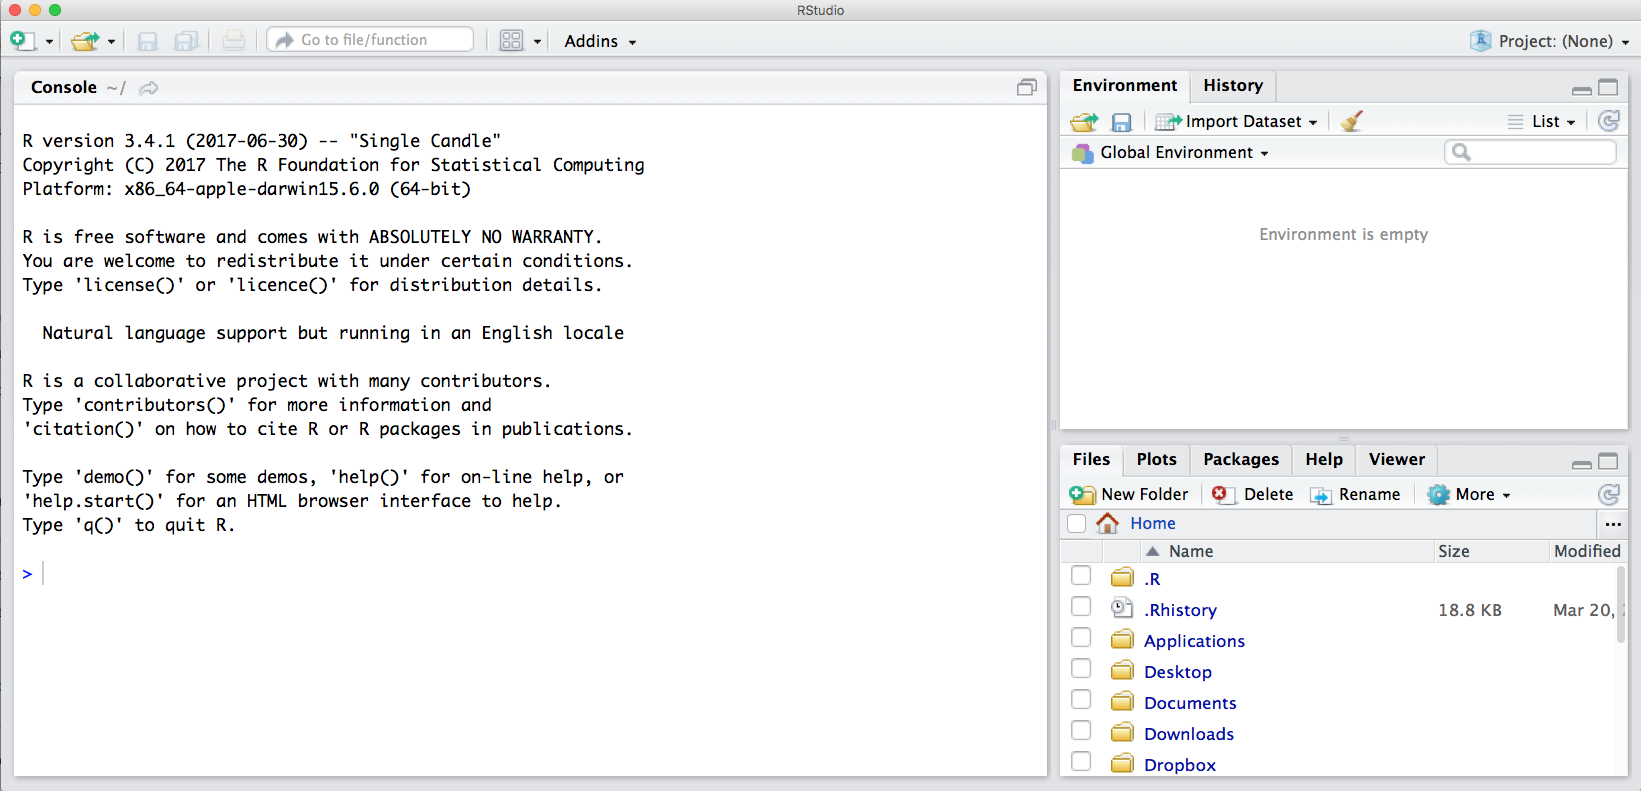
\includegraphics[width=0.8\linewidth]{img/RStudio_IDE}

Notice the default panes:

\begin{itemize}
\tightlist
\item
  Console (entire left)
\item
  Environment/History (tabbed in upper right)
\item
  Files/Plots/Packages/Help (tabbed in lower right)
\end{itemize}

FYI: you can change the default location of the panes, among many other things: \href{https://support.rstudio.com/hc/en-us/articles/200549016-Customizing-RStudio}{Customizing RStudio}.

An important first question: \textbf{where are we?}

If you've have opened RStudio for the first time, you'll be in your Home directory. This is noted by the \texttt{\textasciitilde{}/} at the top of the console. You can see too that the Files pane in the lower right shows what is in the Home directory where you are. You can navigate around within that Files pane and explore, but note that you won't change where you are: even as you click through you'll still be Home: \texttt{\textasciitilde{}/}.

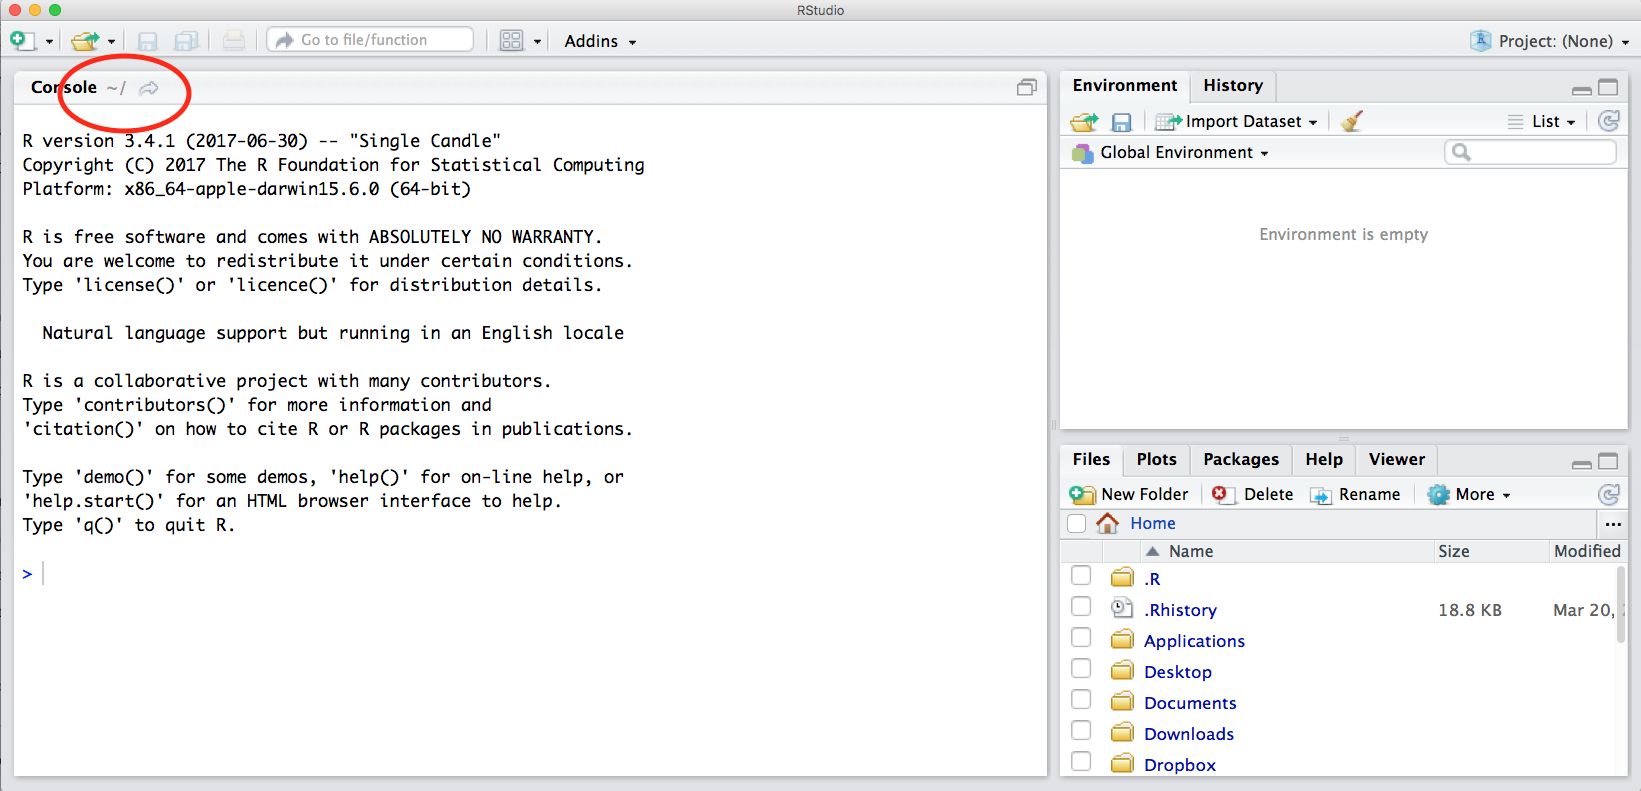
\includegraphics[width=0.8\linewidth]{img/RStudio_IDE_homedir}

\hypertarget{r-console}{%
\subsection{R Console}\label{r-console}}

OK let's go into the Console, where we interact with the live R process.

We can do math:

\begin{Shaded}
\begin{Highlighting}[]
\DecValTok{52}\OperatorTok{*}\DecValTok{40}
\DecValTok{365}\OperatorTok{/}\DecValTok{12}
\end{Highlighting}
\end{Shaded}

But like Excel, the power comes not from doing small operations by hand (like 8*22.3), it's by being able to operate on whole suites of numbers and datasets. In Excel, data are stored in the spreadsheet. In R, they are stored in objects, which are often vectors or dataframes. They are rectangular.

We have to name these dataframes. This is a big difference with Excel, where you usually identify data by its location on the grid, like \texttt{\$A1:D\$20}. (You can do this with Excel by naming ranges of cells, but many people don't do this.)

Data can be a variety of formats, like numeric and text.

\hypertarget{viewing-data-in-r}{%
\subsection{Viewing data in R}\label{viewing-data-in-r}}

Let's have a look at some data in R. Unlike Excel, R comes out-of-the-box with several built-in data sets that we can look at and work with.

One of these datasets is called \texttt{cars}. If I write this in the Console, it will print the data in the console.

\begin{Shaded}
\begin{Highlighting}[]
\NormalTok{cars}
\end{Highlighting}
\end{Shaded}

This returns data. To me this is not super interesting data, but I can appreciate that there are different variables listed as column headers and then numeric values for each type of row observation. (Unfortunately I don't know if these are different cars or trials or conditions but we won't focus on that for now).

I can also use RStudio's Viewer to see this in a more familiar-looking format. Let's type this --- and make sure it's a capital V and open and closed parentheses:

\begin{Shaded}
\begin{Highlighting}[]
\KeywordTok{View}\NormalTok{(cars)}
\end{Highlighting}
\end{Shaded}

This opens the fourth pane of the RStudio IDE; when you work in R you will have all four panes open so this will become a very comforting setup for you.

\begin{quote}
\textbf{\emph{Aside}} The basic R data structure is a vector. You can think of a vector like a column in an Excel spreadsheet with the limitation that all the data in that vector must be of the same type. If it is a character vector, every element must be a character; if it is a logical vector, every element must be TRUE or FALSE; if it's numeric you can trust that every element is a number. There's no such constraint in Excel: you might have a column which has a bunch of numbers, but then some explanatory test intermingled with the numbers. This isn't allowed in R. - \href{https://blog.shotwell.ca/posts/r_for_excel_users/}{Gordon Shotwell}
\end{quote}

In the Viewer I can do things like filter or sort. This does not do anything to the actual data, it just changes how you are viewing the data. So even as I explore it, I am not editing or manipulating the data.

\hypertarget{r-functions-help-pages}{%
\subsection{R functions, help pages}\label{r-functions-help-pages}}

Like Excel, some of the biggest power in R is that there are built-in functions that you can use in your analyses (and, as we'll see, R users can easily create and share functions, and it is this open source developer and contributor community that makes R so awesome).

R has a mind-blowing collection of built-in functions that are used with the same syntax: function name with parentheses around what the function needs to do what it is supposed to do. \texttt{function\_name(argument1\ =\ value1,\ argument2\ =\ value2,\ ...)}. When you see this syntax, we say we are ``calling the function''.

So let's look into some of these functions. In Excel, there is a ``SUM'' function to calculate a total. Let's expect that there is the same in R. I will type this into the Console:

\begin{Shaded}
\begin{Highlighting}[]
\NormalTok{?sum}
\end{Highlighting}
\end{Shaded}

A few important things to note:

\begin{enumerate}
\def\labelenumi{\arabic{enumi}.}
\item
  R is case-sensitive. So ``sum'' is a completely different thing to ``Sum'' or ``SUM''. And this is true for the names of functions, data sets, variable names, and data itself (``blue'' vs ``Blue'').
\item
  RStudio has an autocomplete feature that can help you find the function you're looking for. In many cases it pops up as you type, but you can always type the tab key (above your caps lock key) to prompt the autocomplete. And, bonus: this feature can help you with the case-sensitivity mentioned above: If I start typing ``?SU'' and press tab, it will show me all options starting with those two letters, regardless of capitalization (although it will start with the capital S options).
\end{enumerate}

OK but what does typing \texttt{?sum} actually \emph{do}?

When I press enter/return, it will open up a help page in the bottom right pane. Help pages vary in detail I find some easier to digest than others. But they all have the same structure, which is helpful to know. The help page tells the name of the package in the top left, and broken down into sections:

\begin{itemize}
\tightlist
\item
  Description: An extended description of what the function does.
\item
  Usage: The arguments of the function and their default values.
\item
  Arguments: An explanation of the data each argument is expecting.
\item
  Details: Any important details to be aware of.
\item
  Value: The data the function returns.
\item
  See Also: Any related functions you might find useful.
\item
  Examples: Some examples for how to use the function.
\end{itemize}

When I look at a help page, I start with the description, which might be too in-the-weeds for the level of understanding I need at the offset. For the \texttt{sum} page, it is pretty straight-forward and lets me know that yup, this is the function I want.

I next look at the usage and arguments, which give me a more concrete view into what the function does. This syntax looks a bit cryptic but what it means is that you use it by writing sum, and then passing whatever you want to it in terms of data: that is what the ``\ldots{}'' means. And the ``na.rm=FALSE'' means that by default, it will not remove NAs (I read this as: ``remove NAs? FALSE!'')

Then, I usually scroll down to the bottom to the examples. This is where I can actually see how the function is used, and I can also paste those examples into the Console to see their output. Best way to learn what the function actually does is seeing it in action. Let's try:

\begin{Shaded}
\begin{Highlighting}[]
\KeywordTok{sum}\NormalTok{(}\DecValTok{1}\OperatorTok{:}\DecValTok{5}\NormalTok{)}
\end{Highlighting}
\end{Shaded}

So this is calculating the sum of the numbers from 1 and 5; that is what that \texttt{1:5} syntax means in this case. We can check it with the next example:

\begin{Shaded}
\begin{Highlighting}[]
\KeywordTok{sum}\NormalTok{(}\DecValTok{1}\NormalTok{, }\DecValTok{2}\NormalTok{, }\DecValTok{3}\NormalTok{, }\DecValTok{4}\NormalTok{, }\DecValTok{5}\NormalTok{)}
\end{Highlighting}
\end{Shaded}

Awesome. Let's try this on our \texttt{cars} data

\begin{Shaded}
\begin{Highlighting}[]
\KeywordTok{sum}\NormalTok{(cars)}
\end{Highlighting}
\end{Shaded}

Alright. What is this number? It is the sum of ALL of the data in the \texttt{cars} dataset. Maybe in some analysis this would be a useful operation, but I would worry about the way your data is set up and your analyses if this is ever something you'd want to do. More likely, you'd want to take the sum of a specific column. In R, you can do that with the \texttt{\$} operator.

Let's say we want to calculate the total distance:

\begin{Shaded}
\begin{Highlighting}[]
\KeywordTok{sum}\NormalTok{(cars}\OperatorTok{$}\NormalTok{dist)}
\end{Highlighting}
\end{Shaded}

There are many functions that are built into R, and we'll learn more of them shortly.

Not all functions have (or require) arguments:

\begin{Shaded}
\begin{Highlighting}[]
\KeywordTok{date}\NormalTok{()}
\end{Highlighting}
\end{Shaded}

\begin{verbatim}
## [1] "Thu Dec  5 19:09:32 2019"
\end{verbatim}

\hypertarget{packages}{%
\subsection{Packages}\label{packages}}

So far we've been using a couple functions from base R, such as \texttt{sum()} and \texttt{date()}. But, one of the amazing things about R is that a vast user community is always creating new functions and packages that expand R's capabilities. In R, the fundamental unit of shareable code is the package. A package bundles together code, data, documentation, and tests, and is easy to share with others. They increase the power of R by improving existing base R functionalities, or by adding new ones.

The traditional place to download packages is from CRAN, the \href{https://cran.r-project.org/}{Comprehensive R Archive Network}, which is where you downloaded R. You can also install packages from GitHub, which we'll do tomorrow.

You don't need to go to CRAN's website to install packages, this can be accomplished within R using the command \texttt{install.packages("package-name-in-quotes")}. Let's install a small, fun package \texttt{praise}. You need to use quotes around the package name.

Do this in the Console instead of in your RMarkdown file because we don't want this to load every time:

\begin{Shaded}
\begin{Highlighting}[]
\KeywordTok{install.packages}\NormalTok{(}\StringTok{"praise"}\NormalTok{)}
\end{Highlighting}
\end{Shaded}

Now we've installed the package, but we need to tell R that we are going to use the functions within the \texttt{praise} package. We do this by using the function \texttt{library()}.

In my mind, this is analogous to needing to wire your house for electricity: this is something you do once; this is \texttt{install.packages}. But then you need to turn on the lights each time you need them (R Session).

\begin{Shaded}
\begin{Highlighting}[]
\KeywordTok{library}\NormalTok{(praise)}
\end{Highlighting}
\end{Shaded}

Now that we've loaded the \texttt{praise} package, we can use the single function in the package, \texttt{praise()}, which returns a randomized praise to make you feel better.

\begin{Shaded}
\begin{Highlighting}[]
\KeywordTok{praise}\NormalTok{()}
\end{Highlighting}
\end{Shaded}

\begin{verbatim}
## [1] "You are doozie!"
\end{verbatim}

\hypertarget{assigning-objects-with--}{%
\subsection{\texorpdfstring{Assigning objects with \texttt{\textless{}-}}{Assigning objects with \textless{}-}}\label{assigning-objects-with--}}

This might be a really important value that we want to have on hand. We can save this as its own object. We do this by writing the name along with the assignment operator \texttt{\textless{}-}

\begin{Shaded}
\begin{Highlighting}[]
\NormalTok{sum_dist <-}\StringTok{ }\KeywordTok{sum}\NormalTok{(cars}\OperatorTok{$}\NormalTok{dist)}
\end{Highlighting}
\end{Shaded}

And we can execute it. In my head I hear ``sum\_dist gets 2149''.

Object names can be whatever you want, although they cannot start with a digit and cannot contain certain other characters such as a comma or a space. Different folks have different conventions; you will be wise to adopt a \href{http://en.wikipedia.org/wiki/Snake_case}{convention for demarcating words} in names.

\begin{Shaded}
\begin{Highlighting}[]
\CommentTok{# i_use_snake_case}
\CommentTok{# other.people.use.periods}
\CommentTok{# evenOthersUseCamelCase}
\end{Highlighting}
\end{Shaded}

Notice that as I start typing \texttt{sum\_dist} in the Console, there will be options to auto-fill. This is RStudio helping you out, which is great because we all are prone to typos. I actually have to ignore the help to try to force a typo:

\begin{Shaded}
\begin{Highlighting}[]
\NormalTok{sumdist}
\CommentTok{# Error: object 'sumdist' not found}
\end{Highlighting}
\end{Shaded}

OK this is an error, but I didn't break R --- error messages are your friends.

The first thing to do with an error message is read it. Yes it's in angry red text and it's unexpected --- but most error messages are doing their best to help you solve the problem. And you'll get more familiar with they way they tell you. By saying ``object `sumdist' not found'' alerts me immediately to the fact that this thing I think exists R doesn't think exists --- so maybe it's a typo or not loaded?

\hypertarget{error-messages-are-your-friends}{%
\subsection{Error messages are your friends}\label{error-messages-are-your-friends}}

As \href{https://stat545.com/r-basics.html}{Jenny Bryan says}:

\begin{quote}
Implicit contract with the computer / scripting language: Computer will do tedious computation for you. In return, you will be completely precise in your instructions. Typos matter. Case matters. Pay attention to how you type.
\end{quote}

Remember that this is a language, not unsimilar to English! There are times you aren't understood -- it's going to happen. There are different ways this can happen. Sometimes you'll get an error. This is like someone saying `What?' or `Pardon'? Error messages can also be more useful, like when they say `I didn't understand what you said, I was expecting you to say blah'. That is a great type of error message. Error messages are your friend. Google them (copy-and-paste!) to figure out what they mean.

And also know that there are errors that can creep in more subtly, when you are giving information that is understood, but not in the way you meant. Like if I am telling a story about suspenders that my British friend hears but silently interprets in a very different way (true story). This can leave me thinking I've gotten something across that the listener (or R) might silently interpreted very differently. And as I continue telling my story you get more and more confused\ldots{} Clear communication is critical when you code: write clean, well documented code and check your work as you go to minimize these circumstances!

\hypertarget{logical-operators-and-expressions}{%
\subsection{Logical operators and expressions}\label{logical-operators-and-expressions}}

A moment about \textbf{logical operators and expressions}. We can ask questions about the objects we made. This is not assigning a new value to our \texttt{sum\_dist} object.

\begin{itemize}
\tightlist
\item
  \texttt{==} means `is equal to'
\item
  \texttt{!=} means `is not equal to'
\item
  \texttt{\textless{}} means ` is less than'
\item
  \texttt{\textgreater{}} means ` is greater than'
\item
  \texttt{\textless{}=} means ` is less than or equal to'
\item
  \texttt{\textgreater{}=} means ` is greater than or equal to'
\end{itemize}

\begin{Shaded}
\begin{Highlighting}[]
\NormalTok{sum_dist }\OperatorTok{==}\StringTok{ }\DecValTok{2}
\end{Highlighting}
\end{Shaded}

\begin{verbatim}
## [1] FALSE
\end{verbatim}

\begin{Shaded}
\begin{Highlighting}[]
\NormalTok{sum_dist }\OperatorTok{<=}\StringTok{ }\DecValTok{3000}
\end{Highlighting}
\end{Shaded}

\begin{verbatim}
## [1] TRUE
\end{verbatim}

\begin{Shaded}
\begin{Highlighting}[]
\NormalTok{sum_dist }\OperatorTok{!=}\StringTok{ }\DecValTok{500}
\end{Highlighting}
\end{Shaded}

\begin{verbatim}
## [1] TRUE
\end{verbatim}

\begin{quote}
Shortcuts
You will make lots of assignments and the operator \texttt{\textless{}-} is a pain to type. Don't be lazy and use \texttt{=}, although it would work, because it will just sow confusion later. Instead, utilize \textbf{RStudio's keyboard shortcut: Alt + - (the minus sign)}.
Notice that RStudio automagically surrounds \texttt{\textless{}-} with spaces, which demonstrates a useful code formatting practice. Code is miserable to read on a good day. Give your eyes a break and use spaces.
RStudio offers many handy \href{https://support.rstudio.com/hc/en-us/articles/200711853-Keyboard-Shortcuts}{keyboard shortcuts}. Also, Alt+Shift+K brings up a keyboard shortcut reference card.
\end{quote}

\begin{quote}
My most common shortcuts include command-Z (undo), and combinations of arrow keys in combination with shift/option/command (moving quickly up, down, sideways, with or without highlighting.
\end{quote}

\hypertarget{clearing-the-environment}{%
\section{Clearing the environment}\label{clearing-the-environment}}

Now look at the objects in your environment (workspace) -- in the upper right pane. The workspace is where user-defined objects accumulate.

For reproducibility, it is critical that you delete your objects and restart your R session frequently. You don't want your whole analysis to only work in whatever way you've been working right now --- you need it to work next week, after you upgrade your operating system, etc. Restarting your R session will help you identify and account for anything you need for your analysis.

We will keep coming back to this theme but let's restart our R session together: Go to the top menus: Session \textgreater{} Restart R.

Don't save the workspace!

OK so now that we've got a little bit of a feel for R and RStudio, let's do something much more interesting and really start feeling its power.

\hypertarget{intro-to-rmarkdown}{%
\section{Intro to RMarkdown}\label{intro-to-rmarkdown}}

\hypertarget{what-is-rmarkdown-1-minute-video}{%
\subsection{What is RMarkdown? (1-minute video)}\label{what-is-rmarkdown-1-minute-video}}

Let's watch this to demonstrate all the amazing things you can now do:

\href{https://vimeo.com/178485416}{What is RMarkdown?}

An RMarkdown file will allow us to weave markdown text with chunks of R code to be evaluated and output content like tables and plots.

This is really critical to reproducibility, and it also saves time. This document will recreate your figures for you in the same document where you are writing text. So no more doing analysis, saving a plot, pasting that plot into Word, redoing the analysis, re-saving, re-pasting, etc.

Let's experience this a bit ourselves and then we'll talk about it more.

\hypertarget{create-an-rmarkdown-file}{%
\subsection{Create an RMarkdown file}\label{create-an-rmarkdown-file}}

File -\textgreater{} New File -\textgreater{} RMarkdown\ldots{} -\textgreater{} Document of output format HTML, OK.

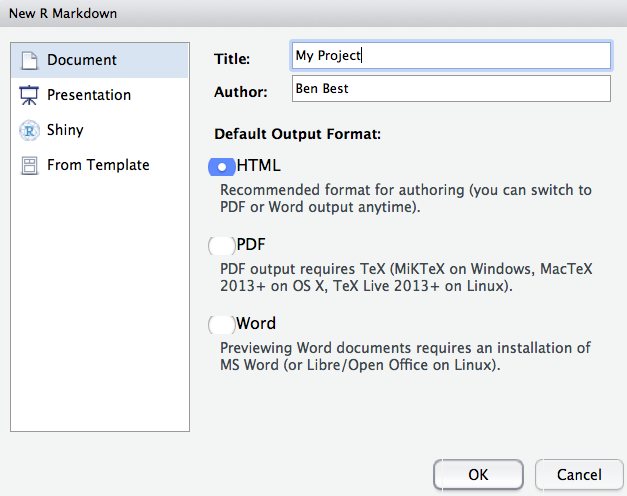
\includegraphics[width=0.8\linewidth]{img/rstudio_new-rmd-doc-html}

You can give it a Title like ``Testing'' (a name that's totally ok to use as you're trying something out). Then click OK.

OK, first off: by opening a file, we are seeing the 4th pane of the RStudio console, which is essentially a text editor. This lets us organize our files within RStudio instead of having a bunch of different windows open.

Let's have a look at this file --- it's not blank; there is some initial text is already provided for you. Notice a few things about it:

\begin{itemize}
\tightlist
\item
  Title and Author are auto-filled, and the today's date has been added
\item
  There are white and grey sections. These are the 2 main languages that make up an RMarkdown file.

  \begin{itemize}
  \tightlist
  \item
    \textbf{Grey sections are R code}
  \item
    \textbf{White sections are Markdown text}
  \end{itemize}
\end{itemize}

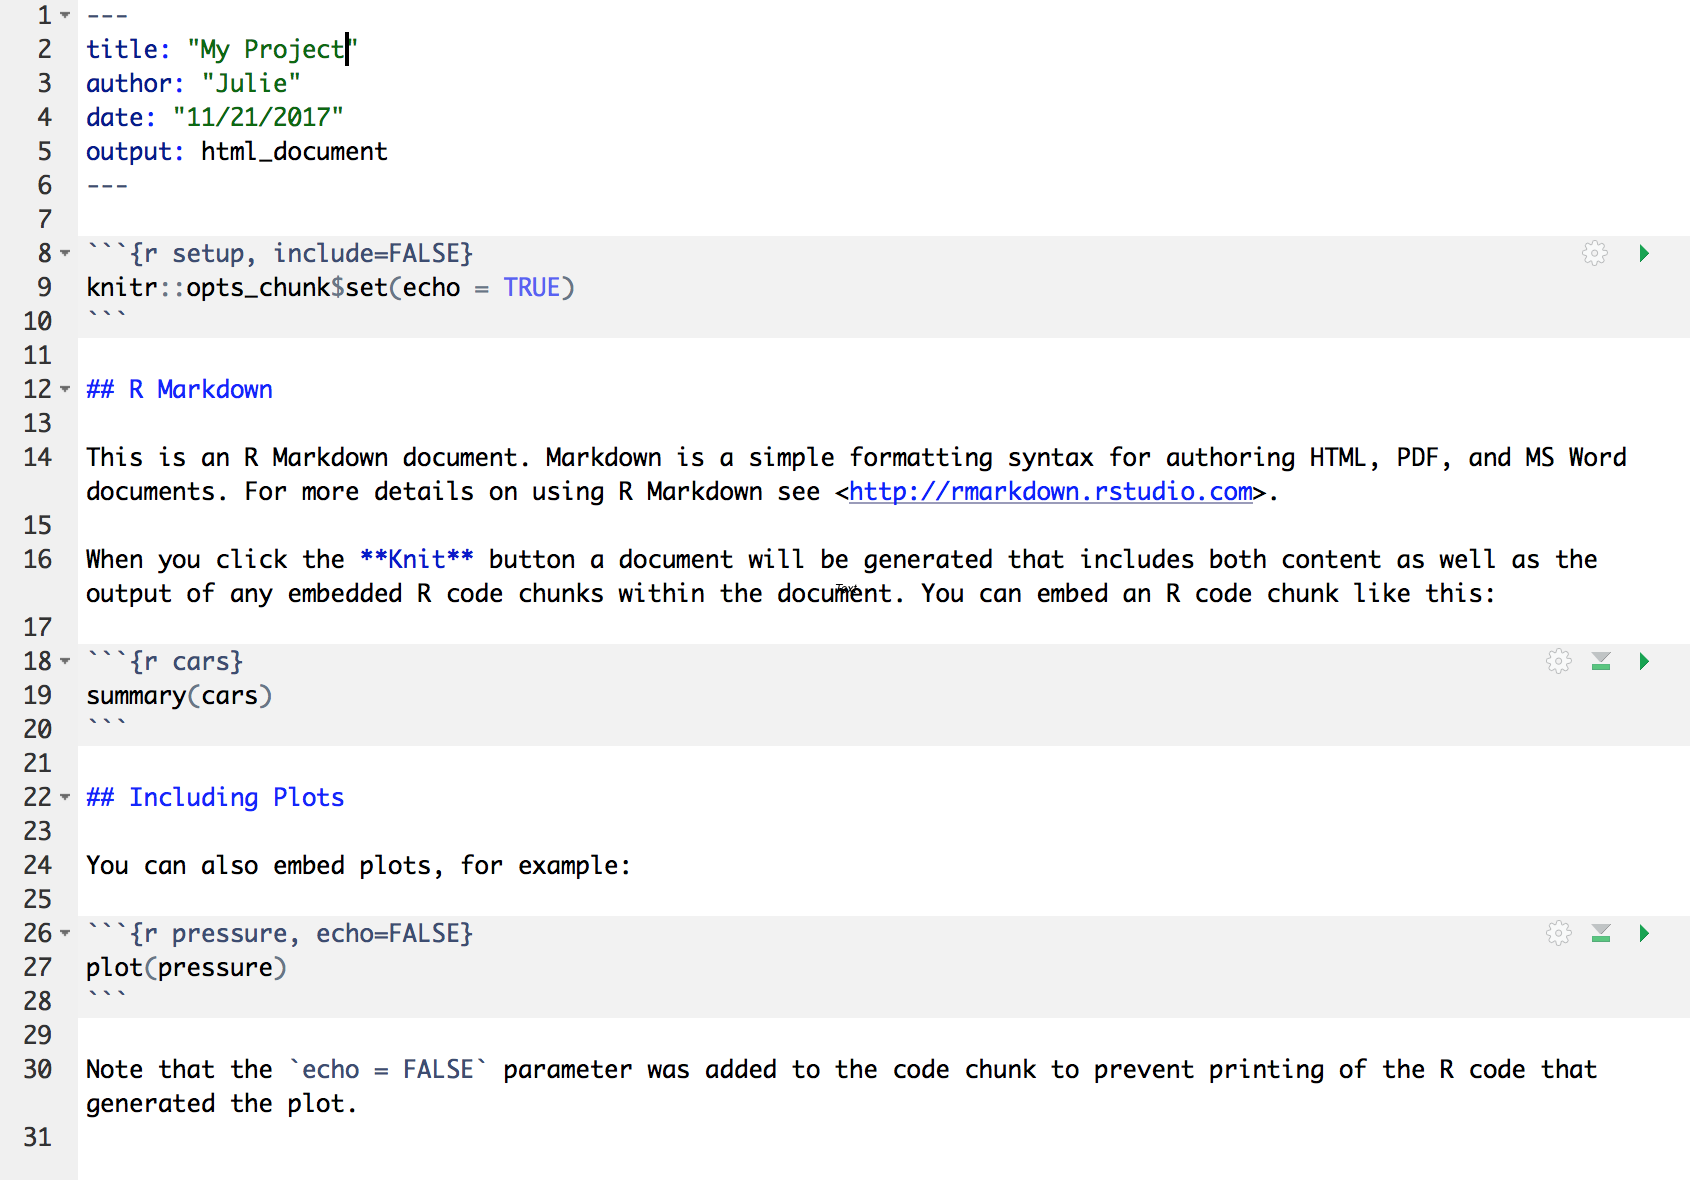
\includegraphics[width=0.8\linewidth]{img/rmarkdown}

\hypertarget{knit-your-rmarkdown-file}{%
\subsection{Knit your RMarkdown file}\label{knit-your-rmarkdown-file}}

Let's go ahead and ``Knit'' by clicking the blue yarn at the top of the RMarkdown file. It's going to ask us to save first, I'll name mine ``testing.Rmd''.

How cool is this, we've just made an html file, a webpage that we are viewing locally on our own computers. Knitting this RMarkdown document has rendered --- we also say formatted --- both the Markdown text (white) and the R code (grey), and the it also executed --- we also say ran --- the R code.

Let's have a look at them side-by-side:

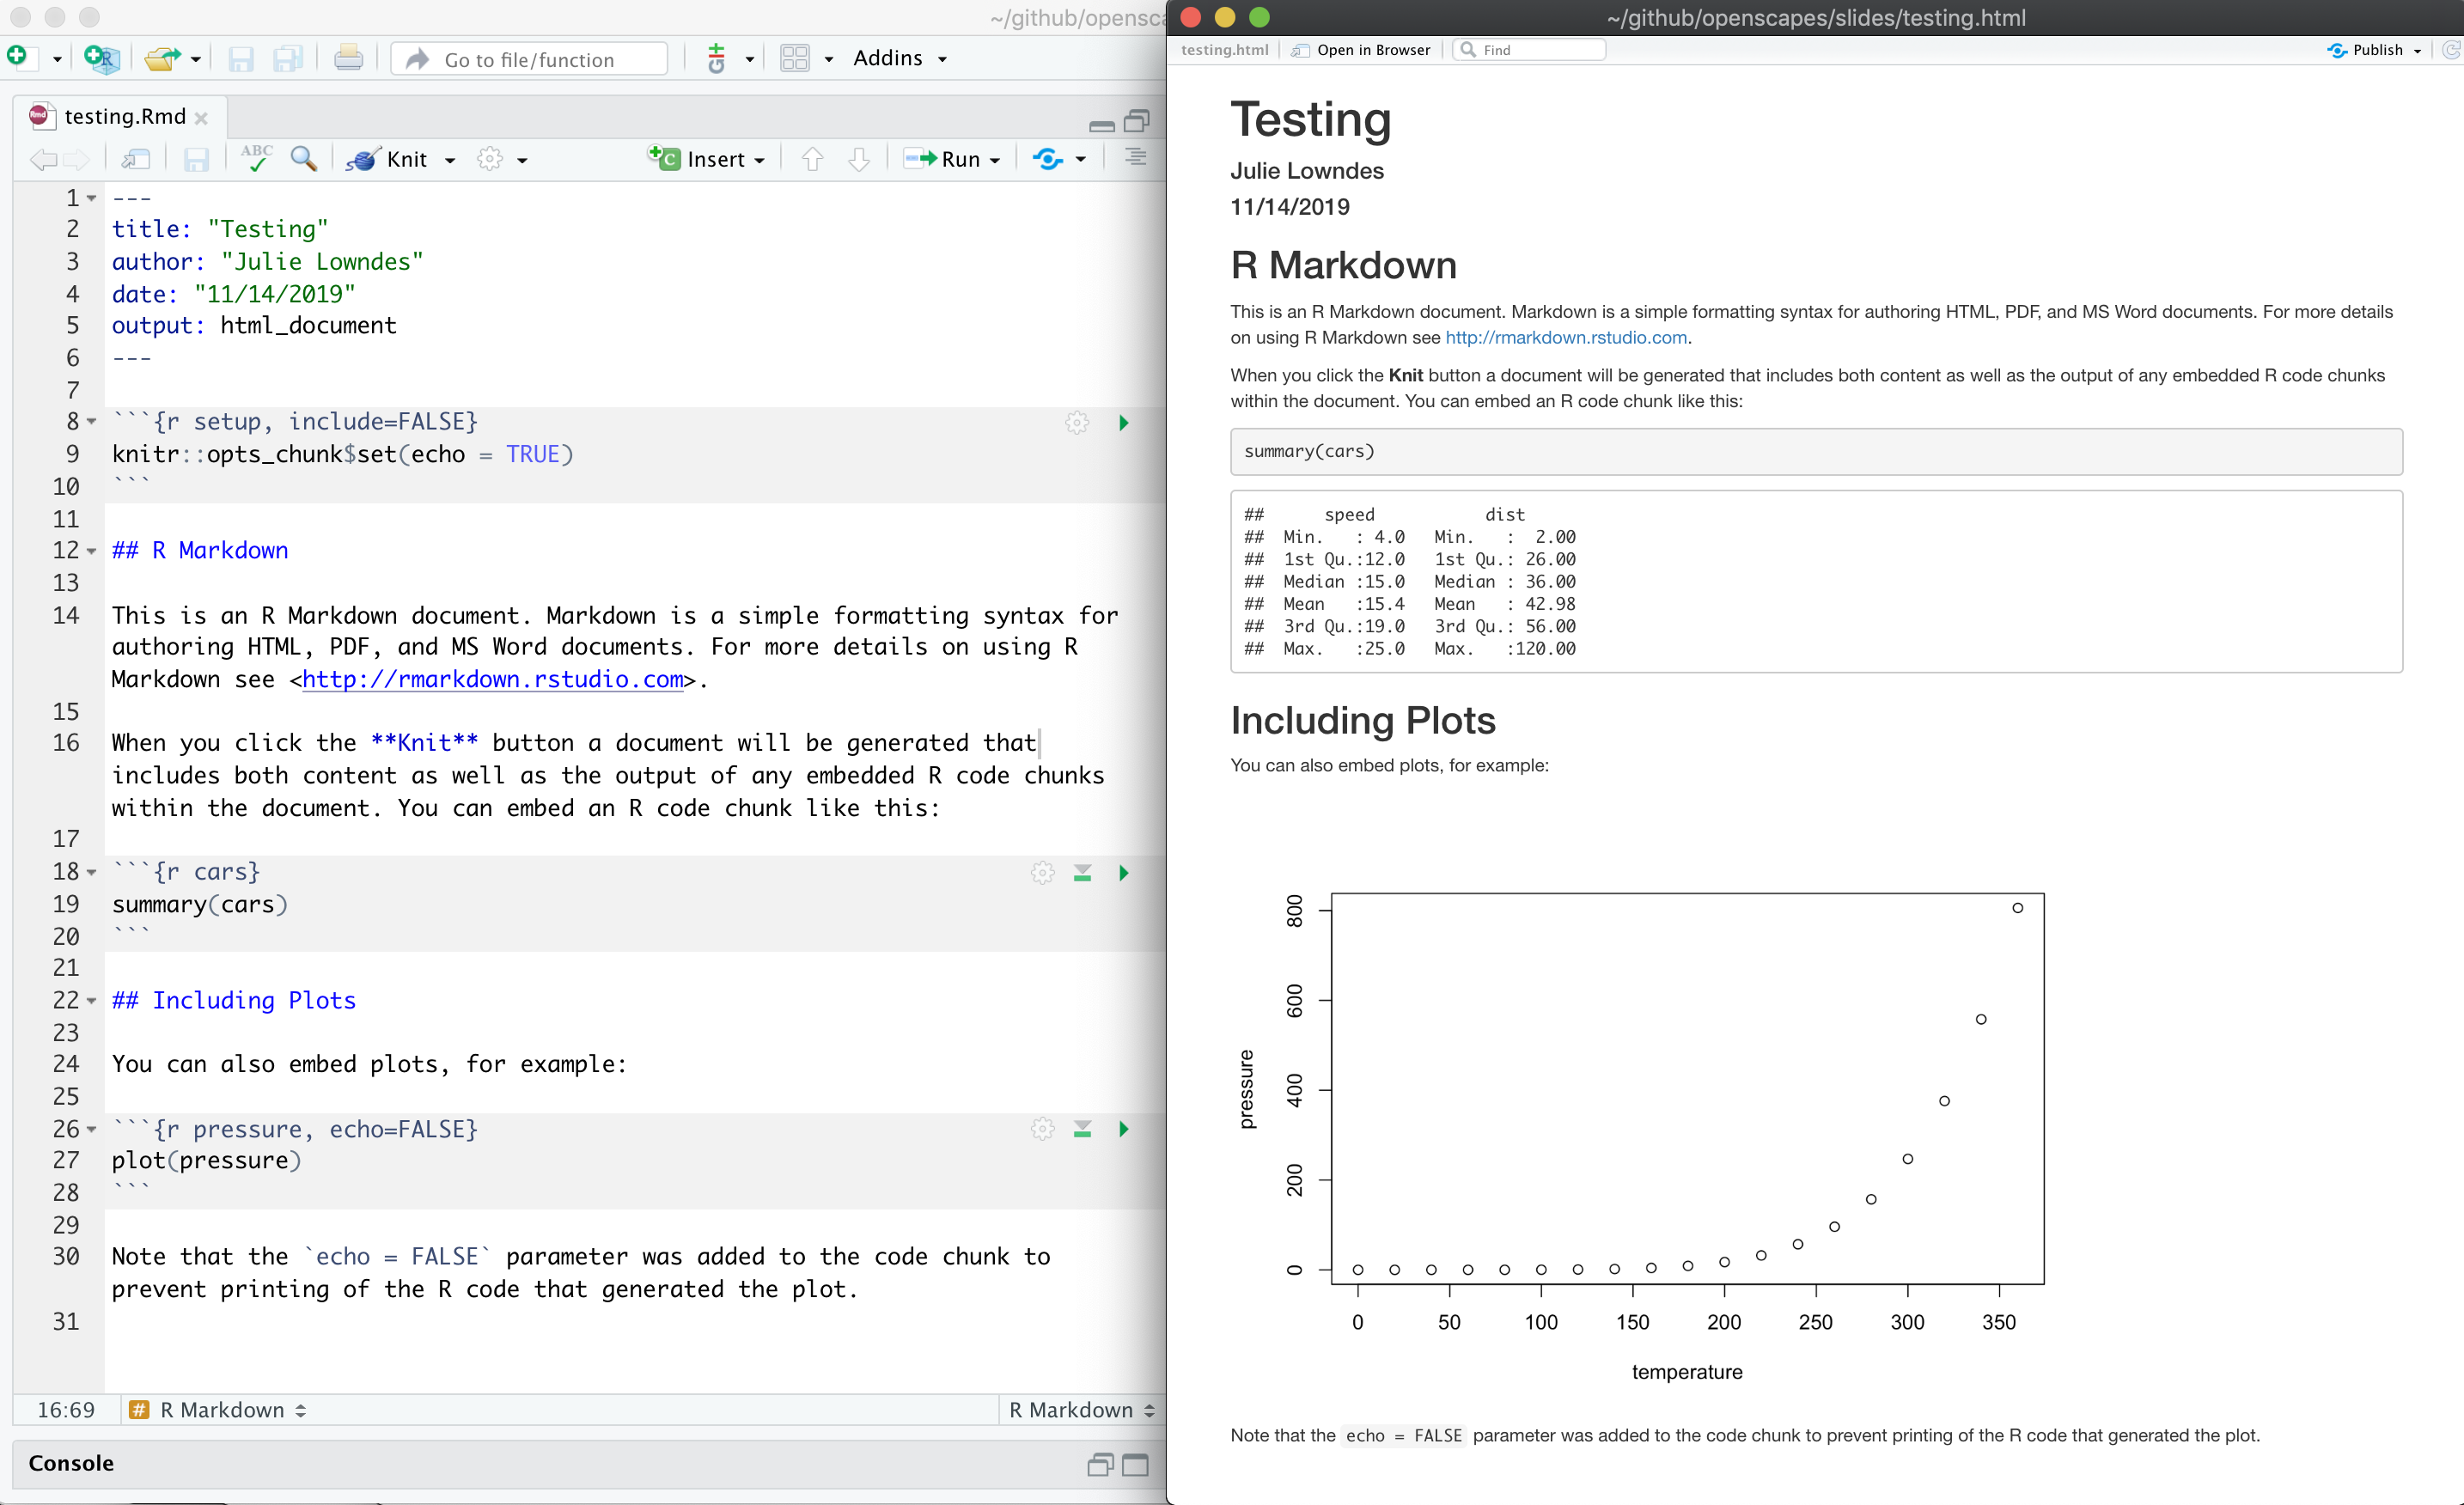
\includegraphics[width=0.8\linewidth]{img/rmarkdown_side_by_side}

Let's take a deeper look at these two files. So much of learning to code is looking for patterns.

\hypertarget{activity-5-mins}{%
\subsection{Activity (5 mins)}\label{activity-5-mins}}

Look at these two files while talking with your neighbor: What do you notice between the two files? Start off with these observations:

\begin{itemize}
\tightlist
\item
  Markdown text (white sections): The two hashtags \texttt{\#\#} cause the following text to be displayed as a header: the text is larger and in bold
\item
  R code (grey sections): The \texttt{summary()} function outputs summary statistics and the \texttt{plot()} function creates a plot!
\end{itemize}

And now let's talk about this.

\hypertarget{r-code-chunks}{%
\subsection{R code chunks}\label{r-code-chunks}}

Notice how the grey \textbf{R code chunks} are surrounded by 3 backticks and \texttt{\{r\ LABEL\}}. These are evaluated and return the output text in the case of \texttt{summary(cars)} and the output plot in the case of \texttt{plot(pressure)}.

Notice how the code \texttt{plot(pressure)} is not shown in the HTML output because of the R code chunk option \texttt{echo=FALSE}.

We can create a new chunk in your RMarkdown first in one of these ways:

\begin{itemize}
\tightlist
\item
  click ``Insert \textgreater{} R'' at the top of the editor pane
\item
  type by hand
  ```\{r\}
  ```
\item
  if you haven't deleted a chunk that came with the new file, edit that one
\end{itemize}

Now, let's write some code in R. Earlier we calculated \texttt{sum(cars\$dist)}. Now let's do the average. In R, this is the \texttt{mean()} function

\begin{Shaded}
\begin{Highlighting}[]
\NormalTok{mean_dist <-}\StringTok{ }\KeywordTok{mean}\NormalTok{(cars}\OperatorTok{$}\NormalTok{dist)}
\end{Highlighting}
\end{Shaded}

Now, hitting return does not execute this command; remember, it's a text file in the text editor, it's not associated with the R engine. To execute it, we need to get what we typed in the the R chunk (the grey R code) down into the console. How do we do it? There are several ways (let's do each of them):

\begin{enumerate}
\def\labelenumi{\arabic{enumi}.}
\tightlist
\item
  copy-paste this line into the console.
\item
  select the line (or simply put the cursor there), and click `Run'. This is available from

  \begin{enumerate}
  \def\labelenumii{\alph{enumii}.}
  \tightlist
  \item
    the bar above the file (green arrow)
  \item
    the menu bar: Code \textgreater{} Run Selected Line(s)
  \item
    keyboard shortcut: command-return
  \end{enumerate}
\item
  click the green arrow at the right of the code chunk
\end{enumerate}

And when we do this, we see the \texttt{mean\_dist} object appear in he Environment pane.

Cool tip: doesn't have to be only R, other languages supported.

\hypertarget{activity-3-min}{%
\subsection{Activity (3 min)}\label{activity-3-min}}

\begin{quote}
Add a few more commands to your file from this morning. Execute your commands by trying the three ways above. Then, knit your R Markdown file, which will also save the Rmd by default.
Remember to write your R code within a code chunk (grey)!
\end{quote}

\hypertarget{markdown-sections}{%
\subsection{Markdown sections}\label{markdown-sections}}

The second language is Markdown. This is a formatting language for plain text, and there are only about 15 rules to know.

Notice the syntax for:

\begin{itemize}
\tightlist
\item
  \textbf{headers} get rendered at multiple levels: \texttt{\#}, \texttt{\#\#}
\item
  \textbf{bold}: \texttt{**word**}
\end{itemize}

There are some good \href{https://github.com/adam-p/markdown-here/wiki/Markdown-Here-Cheatsheet}{cheatsheets} to get you started, and here is one built into RStudio: Go to Help \textgreater{} Markdown Quick Reference

Learn more: \url{http://rmarkdown.rstudio.com/}

\hypertarget{activity}{%
\subsection{Activity}\label{activity}}

\begin{enumerate}
\def\labelenumi{\arabic{enumi}.}
\tightlist
\item
  In Markdown write some italic text, make a numbered list, and add a few subheaders.
  Use the Markdown Quick Reference (in the menu bar: Help \textgreater{} Markdown Quick Reference).
\item
  Reknit your html file.
\end{enumerate}

\hypertarget{restart-r}{%
\subsection{Restart R}\label{restart-r}}

To end our work from this session, save, knit, and then restart R (Go to the top menus: Session \textgreater{} Restart R.)

Notice that now with a clean workspace, if I knit my document instead of sending code to the Console, my objects (like \texttt{mean\_dist}) don't show up in my Environment. This is because R isn't actually running this in this R session, it is actually spinning up a clean session to knit my document. This is important for reproducible analyses because I don't want the success of this analysis to be dependent on some weird setting I have on my computer that will make Future Me or Future Us not able to run or understand these important analyses. Having RMarkdown be self-contained in this way helps you develop good habits for reproducibility.

\hypertarget{deep-thoughts}{%
\section{Deep thoughts}\label{deep-thoughts}}

Comments! Organization (spacing, subsections, vertical structure, indentation, etc.)! Well-named variables! Also, well-named operations so analyses (select(data, columnname)) instead of data{[}1:6,5{]} and excel equivalent. (Ex with strings)
Not so brittle/sensitive to minor changes.

\hypertarget{efficiency-tips}{%
\section{Efficiency Tips}\label{efficiency-tips}}

---\textgreater{}

\hypertarget{github}{%
\chapter{GitHub}\label{github}}

\hypertarget{summary-1}{%
\section{Summary}\label{summary-1}}

We will learn about version control using git and GitHub, and we will interface with this through RStudio. Why use version control? To save time when working with your most important collaborator: you.

\hypertarget{objectives-1}{%
\section{Objectives}\label{objectives-1}}

Today, we'll interface with GitHub from our local computers using RStudio. There are many other ways to interact with GitHub, including GitHub's Desktop App or the command line (\href{http://stat545.com/git02_git-clients.html}{here is Jenny Bryan's list of git clients}), but today we are going to work from RStudio. You have the largest suite of options if you interface through the command line, but the most common things you'll do can be done through one of these other applications (i.e.~RStudio and the GitHub Desktop App).

Here's what we'll do after we set up git on your computers:

\begin{enumerate}
\def\labelenumi{\arabic{enumi}.}
\tightlist
\item
  create a repository on Github.com
\item
  clone locally using RStudio
\item
  learn the RStudio-GitHub workflow by syncing to Github.com: pull, stage, commit, push
\item
  explore github.com: files, commit history, file history
\item
  practice the RStudio-GitHub workflow by editing and adding files
\item
  practice R Markdown
\end{enumerate}

git will track and version your files, GitHub stores this online and enables you to collaborate with others (and yourself). Although git and GitHub are two different things, distinct from each other, we can think of them as a bundle since we will always use them together. It also helped me to think of GitHub like Dropbox: you make folders that are `tracked' and can be synced to the cloud. GitHub does this too, but you have to be more deliberate about when syncs are made. This is because GitHub saves these as different versions, with information about who contributed when, line-by-line. This makes collaboration easier, and it allows you to roll-back to different versions or contribute to others' work.

\hypertarget{resources-2}{%
\section{Resources}\label{resources-2}}

These materials borrow from:

\begin{itemize}
\tightlist
\item
  Jenny Bryan's lectures from STAT545 at UBC: \href{http://stat545.com/git09_shell.html}{The Shell}
\item
  Jenny Bryan's \href{http://happygitwithr.com}{Happy git with R} tutorial
\item
  Melanie Frazier's \href{https://rawgit.com/nazrug/Quickstart/master/GithubQuickstart.html}{GitHub Quickstart}, \href{https://github.com/OHI-Science/data-science-training/blob/master/github_mel.Rmd}{GitHub Lesson at University of Queensland}
\item
  Ben Best's \href{http://remi-daigle.github.io/2016-04-15-UCSB/git/}{Software Carpentry at UCSB}
\end{itemize}

Today, we'll only introduce the features and terminology that scientists need to learn to begin managing their projects.

\hypertarget{why-should-r-users-use-github}{%
\section{Why should R users use Github?}\label{why-should-r-users-use-github}}

\begin{enumerate}
\def\labelenumi{\arabic{enumi}.}
\tightlist
\item
  Ends (or, nearly ends) the horror of keeping track of versions.
  Basically, we get away from this:
  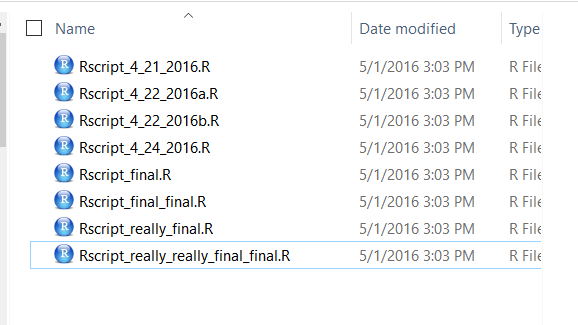
\includegraphics{img/MessySaves.png}
  When you open your repository, you only see the most recent version. But, it easy to compare versions, and you can easily revert to previous versions.
\item
  Improves collaborative efforts. Different researchers can work on the same files at the same time!
\item
  It is easy to share and distribute files through the Github website.
\item
  Your files are available anywhere, you just need internet connection!
\end{enumerate}

\hypertarget{what-are-git-and-github}{%
\subsection{What are Git and Github?}\label{what-are-git-and-github}}

\begin{itemize}
\item
  \textbf{Git} is a version control system that lets you track changes to files over time. These files can be any kind of file (eg .doc, .pdf, .xls), but free text differences are most easily visible (eg txt, csv, md).
\item
  \textbf{Github} is a website for storing your git versioned files remotely. It has many nice features to be able visualize differences between \href{https://help.github.com/articles/rendering-and-diffing-images/}{images}, \href{https://help.github.com/articles/mapping-geojson-files-on-github/}{rendering} \& \href{https://github.com/blog/1772-diffable-more-customizable-maps}{diffing} map data files, \href{https://help.github.com/articles/rendering-csv-and-tsv-data/}{render text data files}, and \href{https://help.github.com/articles/rendering-differences-in-prose-documents/}{track changes in text}.
\end{itemize}

\begin{quote}
If you are a student you can get the micro account which includes 5 private repositories for free (normally a \$7/month value). You can sign up for the student account \href{https://education.github.com/pack}{here}. Instructors can also request a free organization \href{https://education.github.com/}{account, ``Request a discount''}.
\end{quote}

Github was developed for social coding (i.e., sort of like an open source Wikipedia for programmers). Consequently, much of the functionality and terminology of Github (e.g., branches and pull requests) isn't necessary for a scientist getting started.

These concepts are more important for coders who want the entire coding community (and not just people working on the same project) to be able to suggest changes to their code. This isn't how most scientists will use Github.

To get the full functionality of Github, you will eventually want to learn other concepts. But, this can wait.

\hypertarget{some-github-terminology}{%
\subsection{Some Github terminology}\label{some-github-terminology}}

\begin{itemize}
\tightlist
\item
  \textbf{User}: A Github account for you (e.g., jules32).
\item
  \textbf{Organization}: The Github account for one or more user (e.g., datacarpentry).
\item
  \textbf{Repository}: A folder within the organization that includes files dedicated to a project.
\item
  \textbf{Local Github}: Copies of Github files located your computer.
\item
  \textbf{Remote Github}: Github files located on the \url{https://github.com} website.
\item
  \textbf{Clone}: Process of making a local copy of a remote Github repository. This only needs to be done once (unless you mess up your local copy).
\item
  \textbf{Pull}: Copy changes on the remote Github repository to your local Github repository. This is useful if multiple people are making changes to a repository.
\item
  \textbf{Push}: Save local changes to remote Github
\end{itemize}

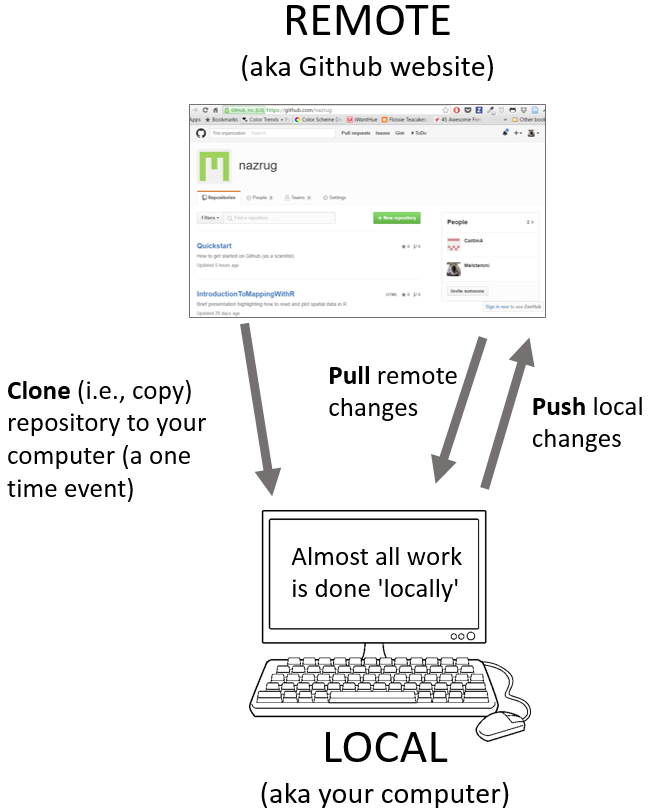
\includegraphics{img/push_pull_clone.png}

\hypertarget{setup-git-github}{%
\section{Setup Git \& GitHub}\label{setup-git-github}}

We're going to switch gears from R for a moment and set up Git and GitHub, which we will be using along with R and RStudio for the rest of the workshop. This set up is a one-time thing! You will only have to do this once per computer. We'll walk through this together.

\begin{enumerate}
\def\labelenumi{\arabic{enumi}.}
\item
  Create \textbf{Github} account at \url{http://github.com}, if you don't already have one. For username, I recommend all lower-case letters, short as you can. I recommend using your \emph{.edu email}, since you can request free private repositories via \href{https://education.github.com/}{GitHub Education} discount.
\item
  You will use the \texttt{usethis} package to configure \textbf{git} with global commands, which means it will apply `globally' to all files on your computer, rather than to a specific folder.
\end{enumerate}

\begin{Shaded}
\begin{Highlighting}[]
\KeywordTok{install.packages}\NormalTok{(}\StringTok{"usethis"}\NormalTok{)}
\KeywordTok{library}\NormalTok{(usethis)}

\KeywordTok{use_git_config}\NormalTok{(}\DataTypeTok{user.name =} \StringTok{"Melsteroni"}\NormalTok{, }\DataTypeTok{user.email =} \StringTok{"Melsteroni@example.org"}\NormalTok{)}
\end{Highlighting}
\end{Shaded}

\emph{BACKUP PLAN} If \texttt{usethis} fails, the following is the classic approach to configuring \textbf{git}. Open the Git Bash program (Windows) or the Terminal (Mac) and type the following:

\begin{verbatim}
    # display your version of git
    git --version
    
    # replace USER with your Github user account
    git config --global user.name USER
    
    # replace NAME@EMAIL.EDU with the email you used to register with Github
    git config --global user.email NAME@EMAIL.EDU
    
    # list your config to confirm user.* variables set
    git config --list
\end{verbatim}

Not only have you just set up git as a one-time-only thing, you have just used the command line. We don't have time to learn much of the command line today, but you just successfully used it following explicit instructions, which is huge! There are great resources for learning the command line, check out \href{http://remi-daigle.github.io/2016-04-15-UCSB/shell/}{this tutorial from SWC at UCSB}.

\hypertarget{troubleshooting}{%
\subsection{Troubleshooting}\label{troubleshooting}}

If you have problems setting up git, please see the \href{http://happygitwithr.com/troubleshooting.html}{Troubleshooting section} in Jenny Bryan's amazing \href{http://happygitwithr.com}{HappyGitWithR}.

\hypertarget{newish-error-on-a-mac}{%
\subsubsection{New(ish) Error on a Mac}\label{newish-error-on-a-mac}}

We've also seen the following errors from RStudio:

\begin{verbatim}
error key does not contain a section --global terminal
\end{verbatim}

and

\begin{verbatim}
fatal: not in a git directory
\end{verbatim}

To solve this, go to the Terminal and type:
\texttt{which\ git}

Look at the filepath that is returned. Does it say anything to do with Apple?

-\textgreater{} If yes, then the \href{https://git-scm.com/downloads}{Git you downloaded} isn't installed, please redownload if necessary, and follow instructions to install.

-\textgreater{} If no, (in the example image, the filepath does not say anything with Apple) then proceed below:

In RStudio, navigate to: Tools \textgreater{} Global Options \textgreater{} Git/SVN.

Does the \textbf{``Git executable''} filepath match what the url in Terminal says?

If not, click the browse button and navigate there.

\begin{quote}
\emph{Note}: on my laptop, even though I navigated to /usr/local/bin/git, it then automatically redirect because /usr/local/bin/git was an alias on my computer. That is fine. Click OK.
\end{quote}

Quit RStudio.

Then relaunch RStudio.

Try syncing or cloning, and if that works and then you don't need to worry about typing into the Terminal, you're all done!

\hypertarget{create-a-repository-on-github.com}{%
\section{Create a repository on Github.com}\label{create-a-repository-on-github.com}}

First, go to your account on github.com and click ``New repository''.
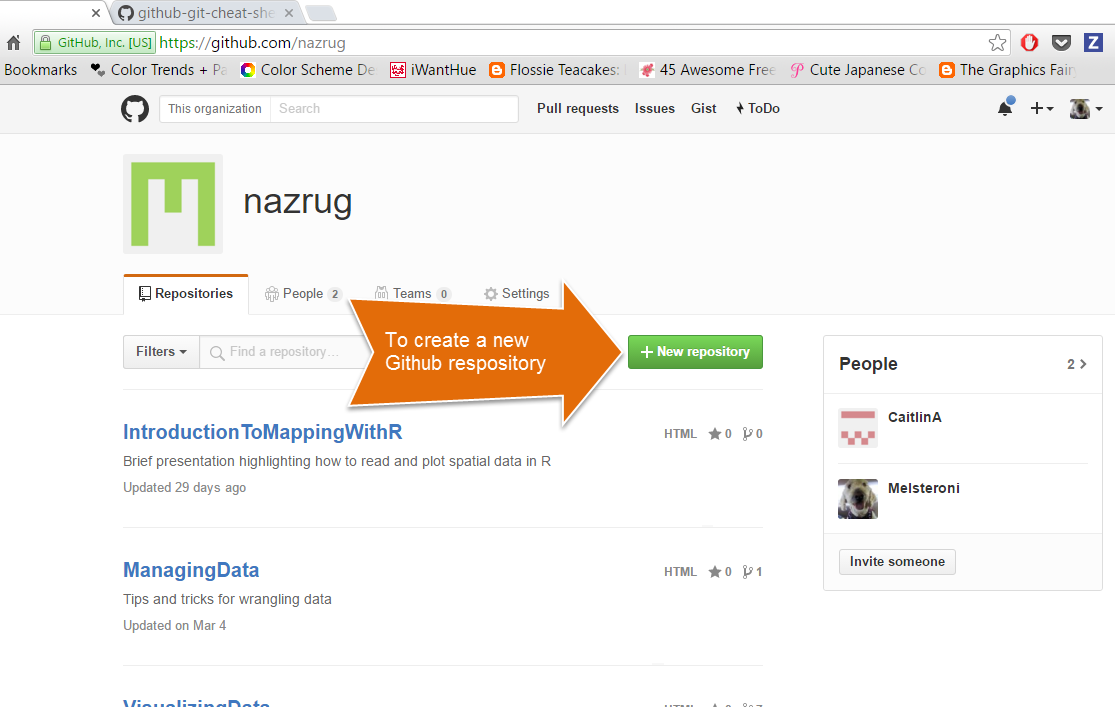
\includegraphics{img/create_repository.png}

Choose a name. Call it whatever you want (the shorter the better), or follow me for convenience. I will call mine \texttt{r-workshop}.

Also, add a description, make it public, create a README file, and create your repo!
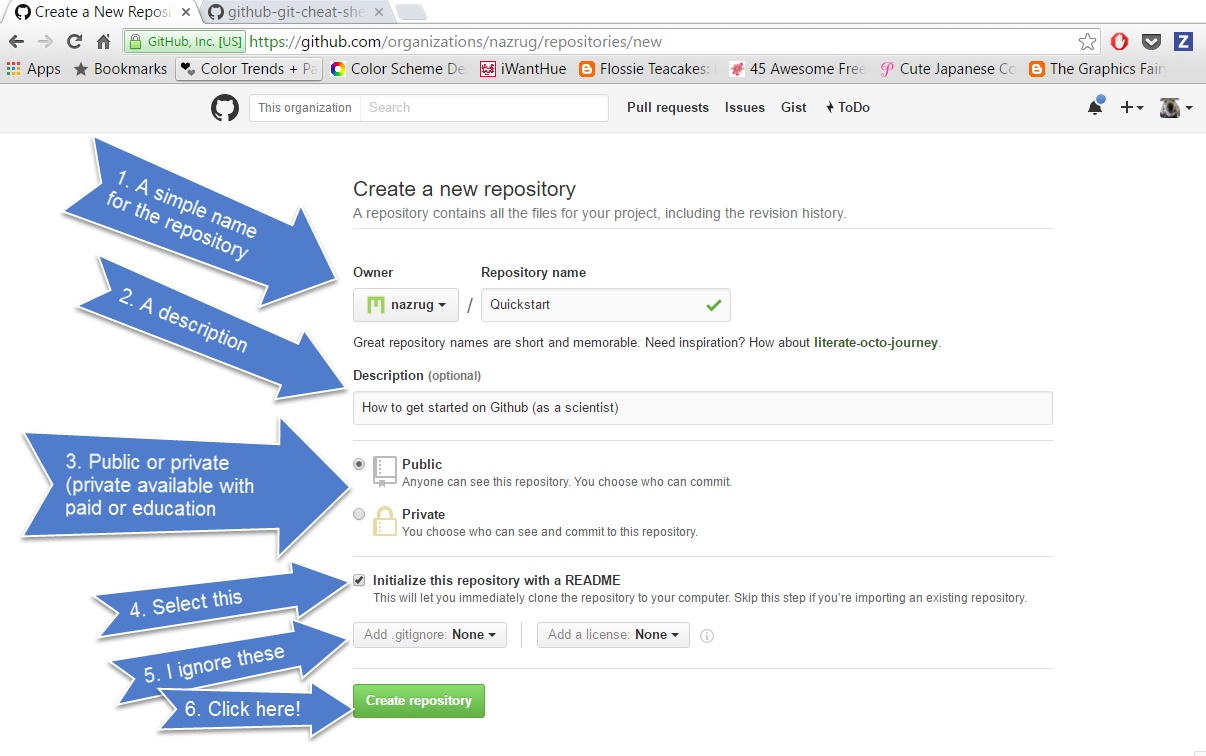
\includegraphics{img/create_repository_2.png}

The \emph{Add gitignore} option adds a document where you can identify files or file-types you want Github to ignore. These files will stay in on the local Github folder (the one on your computer), but will not be uploaded onto the web version of Github.

The \emph{Add a license} option adds a license that describes how other people can use your Github files (e.g., open source, but no one can profit from them, etc.). We won't worry about this today.

Check out our new repository!

Notice how the README.md file we created is automatically displayed at the bottom. The .md means that it is Markdown (remember how .Rmd was RMarkdown?) so the formatting we learned in the last lesson apply here.

\includegraphics{img/new_repository.png}

\hypertarget{create-a-gh-pages-branch}{%
\section{Create a gh-pages branch}\label{create-a-gh-pages-branch}}

We aren't going to talk about branches very much, but they are a powerful feature of git/GitHub. I think of it as creating a copy of your work that becomes a parallel universe that you can modify safely because it's not affecting your original work. And then you can choose to merge the universes back together if and when you want. By default, when you create a new repo you begin with one branch, and it is named \texttt{master}. When you create new branches, you can name them whatever you want. However, if you name one \texttt{gh-pages} (all lowercase, with a \texttt{-} and no spaces), this will let you create a website. And that's our plan. So, let's do this to create a \texttt{gh-pages} branch:

On the homepage for your repo on GitHub.com, click the button that says ``Branch:master''. Here, you can switch to another branch (right now there aren't any others besides \texttt{master}), or create one by typing a new name.

Let's type \texttt{gh-pages}.

Let's also change \texttt{gh-pages} to the default branch and delete the master branch: this will be a one-time-only thing that we do here:

First click to control branches:

And then click to change the default branch to \texttt{gh-pages}. I like to then delete the \texttt{master} branch when it has the little red trash can next to it. It will make you confirm that you really want to delete it, which I do!

\textbf{From here, you will work locally (on your computer).}

\hypertarget{clone-your-repository-using-rstudio}{%
\section{Clone your repository using RStudio}\label{clone-your-repository-using-rstudio}}

We'll start of by cloning to our local computer using RStudio. We are going to be cloning a copy of our Remote repository on Github.com to our local computers. Unlike downloading, cloning keeps all the version control and user information bundled with the files.

\textbf{Step 0}: Create your \texttt{github} folder

This is really important! We need to be organized and deliberate about where we want to keep all of our GitHub repositories (since this is the first of many in your career).

Let's all make a folder called \texttt{github} (all lowercase!) in our home directories. So it will look like this:

\begin{itemize}
\tightlist
\item
  Windows: \texttt{Users\textbackslash{}{[}User{]}\textbackslash{}Documents\textbackslash{}github\textbackslash{}}
\item
  Mac: \texttt{Users/{[}User{]}/github/}
\end{itemize}

This will let us take advantage of something that is really key about GitHub.com: you can easily navigate through folders within repositories and the urls reflect this navigation. The greatness of this will be evident soon. So let's set ourselves up for easily translating (and remembering) those navigation paths by having a folder called \texttt{github} that will serve as our `github.com'.

So really. Make sure that you have an all-lowercase folder called \texttt{github} in your home directory!!

\textbf{Step 1}: Copy the web address of the repository you want to clone.

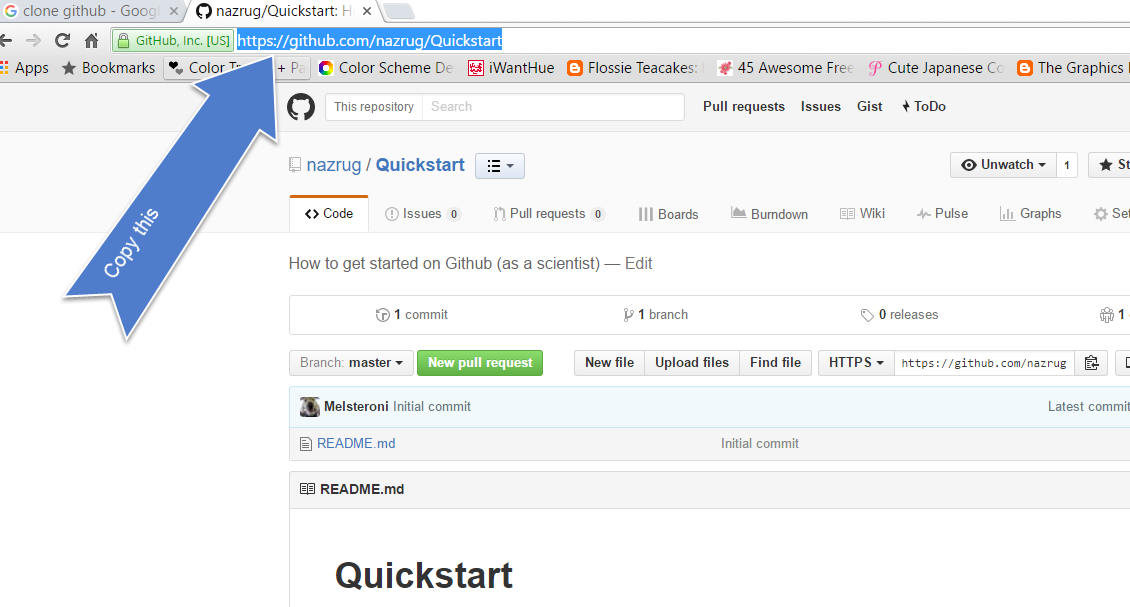
\includegraphics{img/clone_step1.png}

\textbf{Step 2}: from RStudio, go to New Project (also in the File menu).

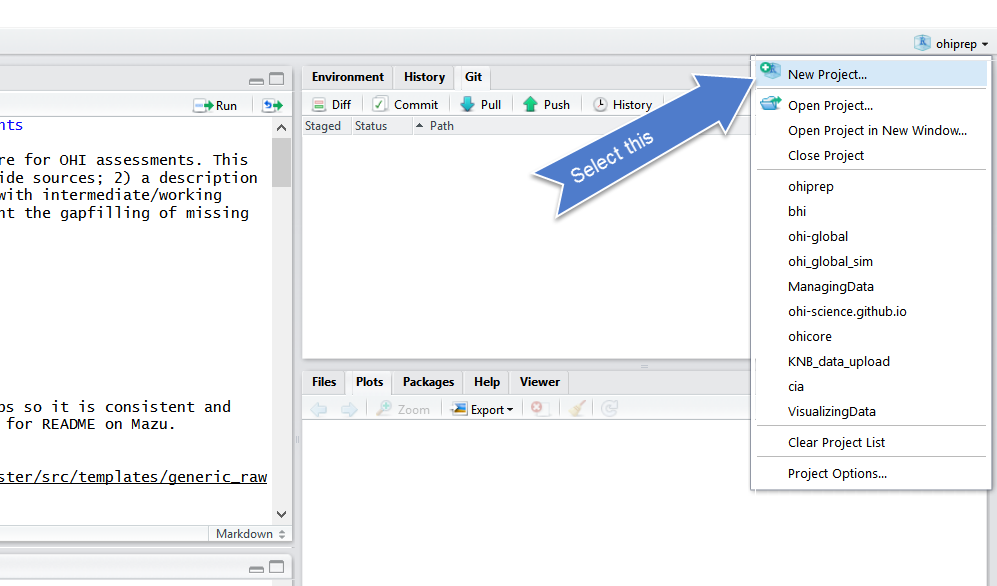
\includegraphics{img/new_project_1.png}

\textbf{Step 3}: Select Version Control

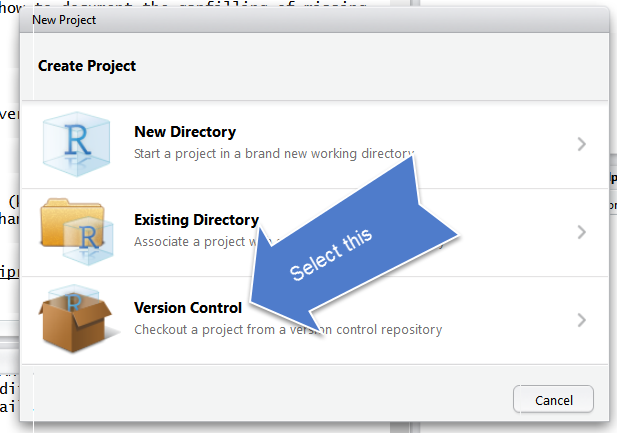
\includegraphics{img/new_project_2.png}

\textbf{Step 4}: Select Git

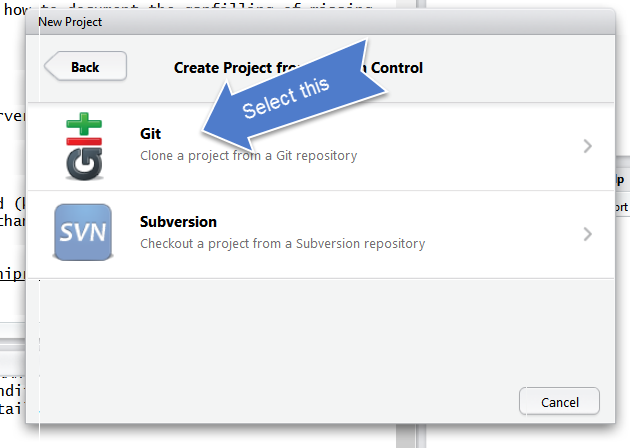
\includegraphics{img/new_project_3.png}

\textbf{Step 5}: Paste it in the Repository URL field, and type \textbf{tab} to autofill the Project Directory name. Make sure you keep the Project Directory Name \textbf{THE SAME} as the repository name from the URL.

Save it in your github folder (click on Browse) to do this.

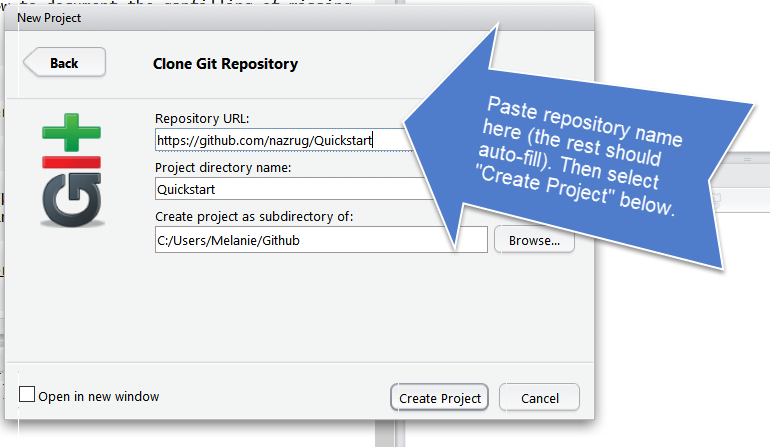
\includegraphics{img/new_project_4.png}

If everything went well, the repository will be added to the list located here:
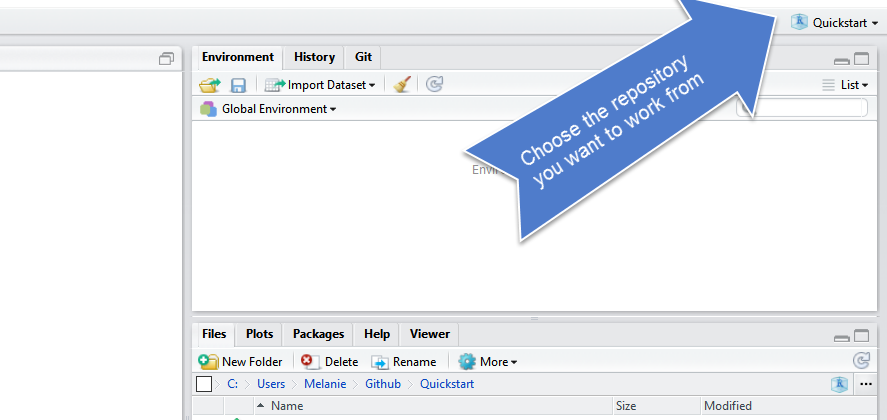
\includegraphics{img/select_project.png}

And the repository will be saved to the Github folder on your computer:

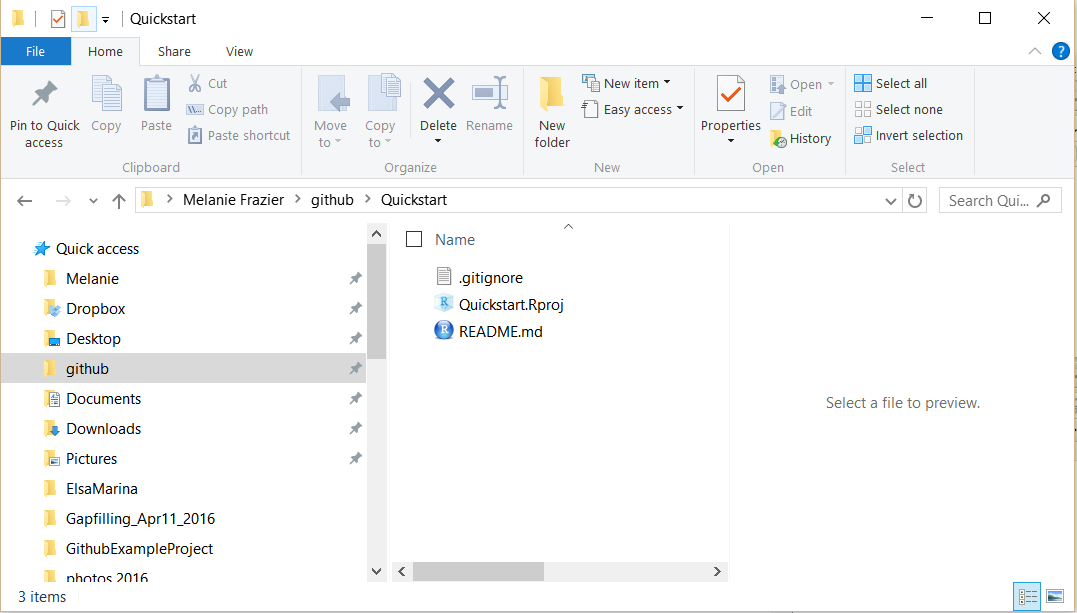
\includegraphics{img/cloned_repository.png}

Ta da!!!! The folder doesn't contain much of interest, but we are going to change that.

\hypertarget{inspect-your-repository}{%
\section{Inspect your repository}\label{inspect-your-repository}}

Notice a few things in our repo here:

\begin{enumerate}
\def\labelenumi{\arabic{enumi}.}
\tightlist
\item
  Our working directory is set to \texttt{\textasciitilde{}/github/r-workshop}. This means that I can start working with the files I have in here without setting the filepath. This is that when we cloned this from RStudio, it created an RStudio project, which you can tell because:

  \begin{itemize}
  \tightlist
  \item
    \texttt{.RProj} file, which you can see in the Files pane.
  \item
    The project is named in the top right hand corner
  \end{itemize}
\item
  We have a git tab! This is how we will interface directly to Github.com
\end{enumerate}

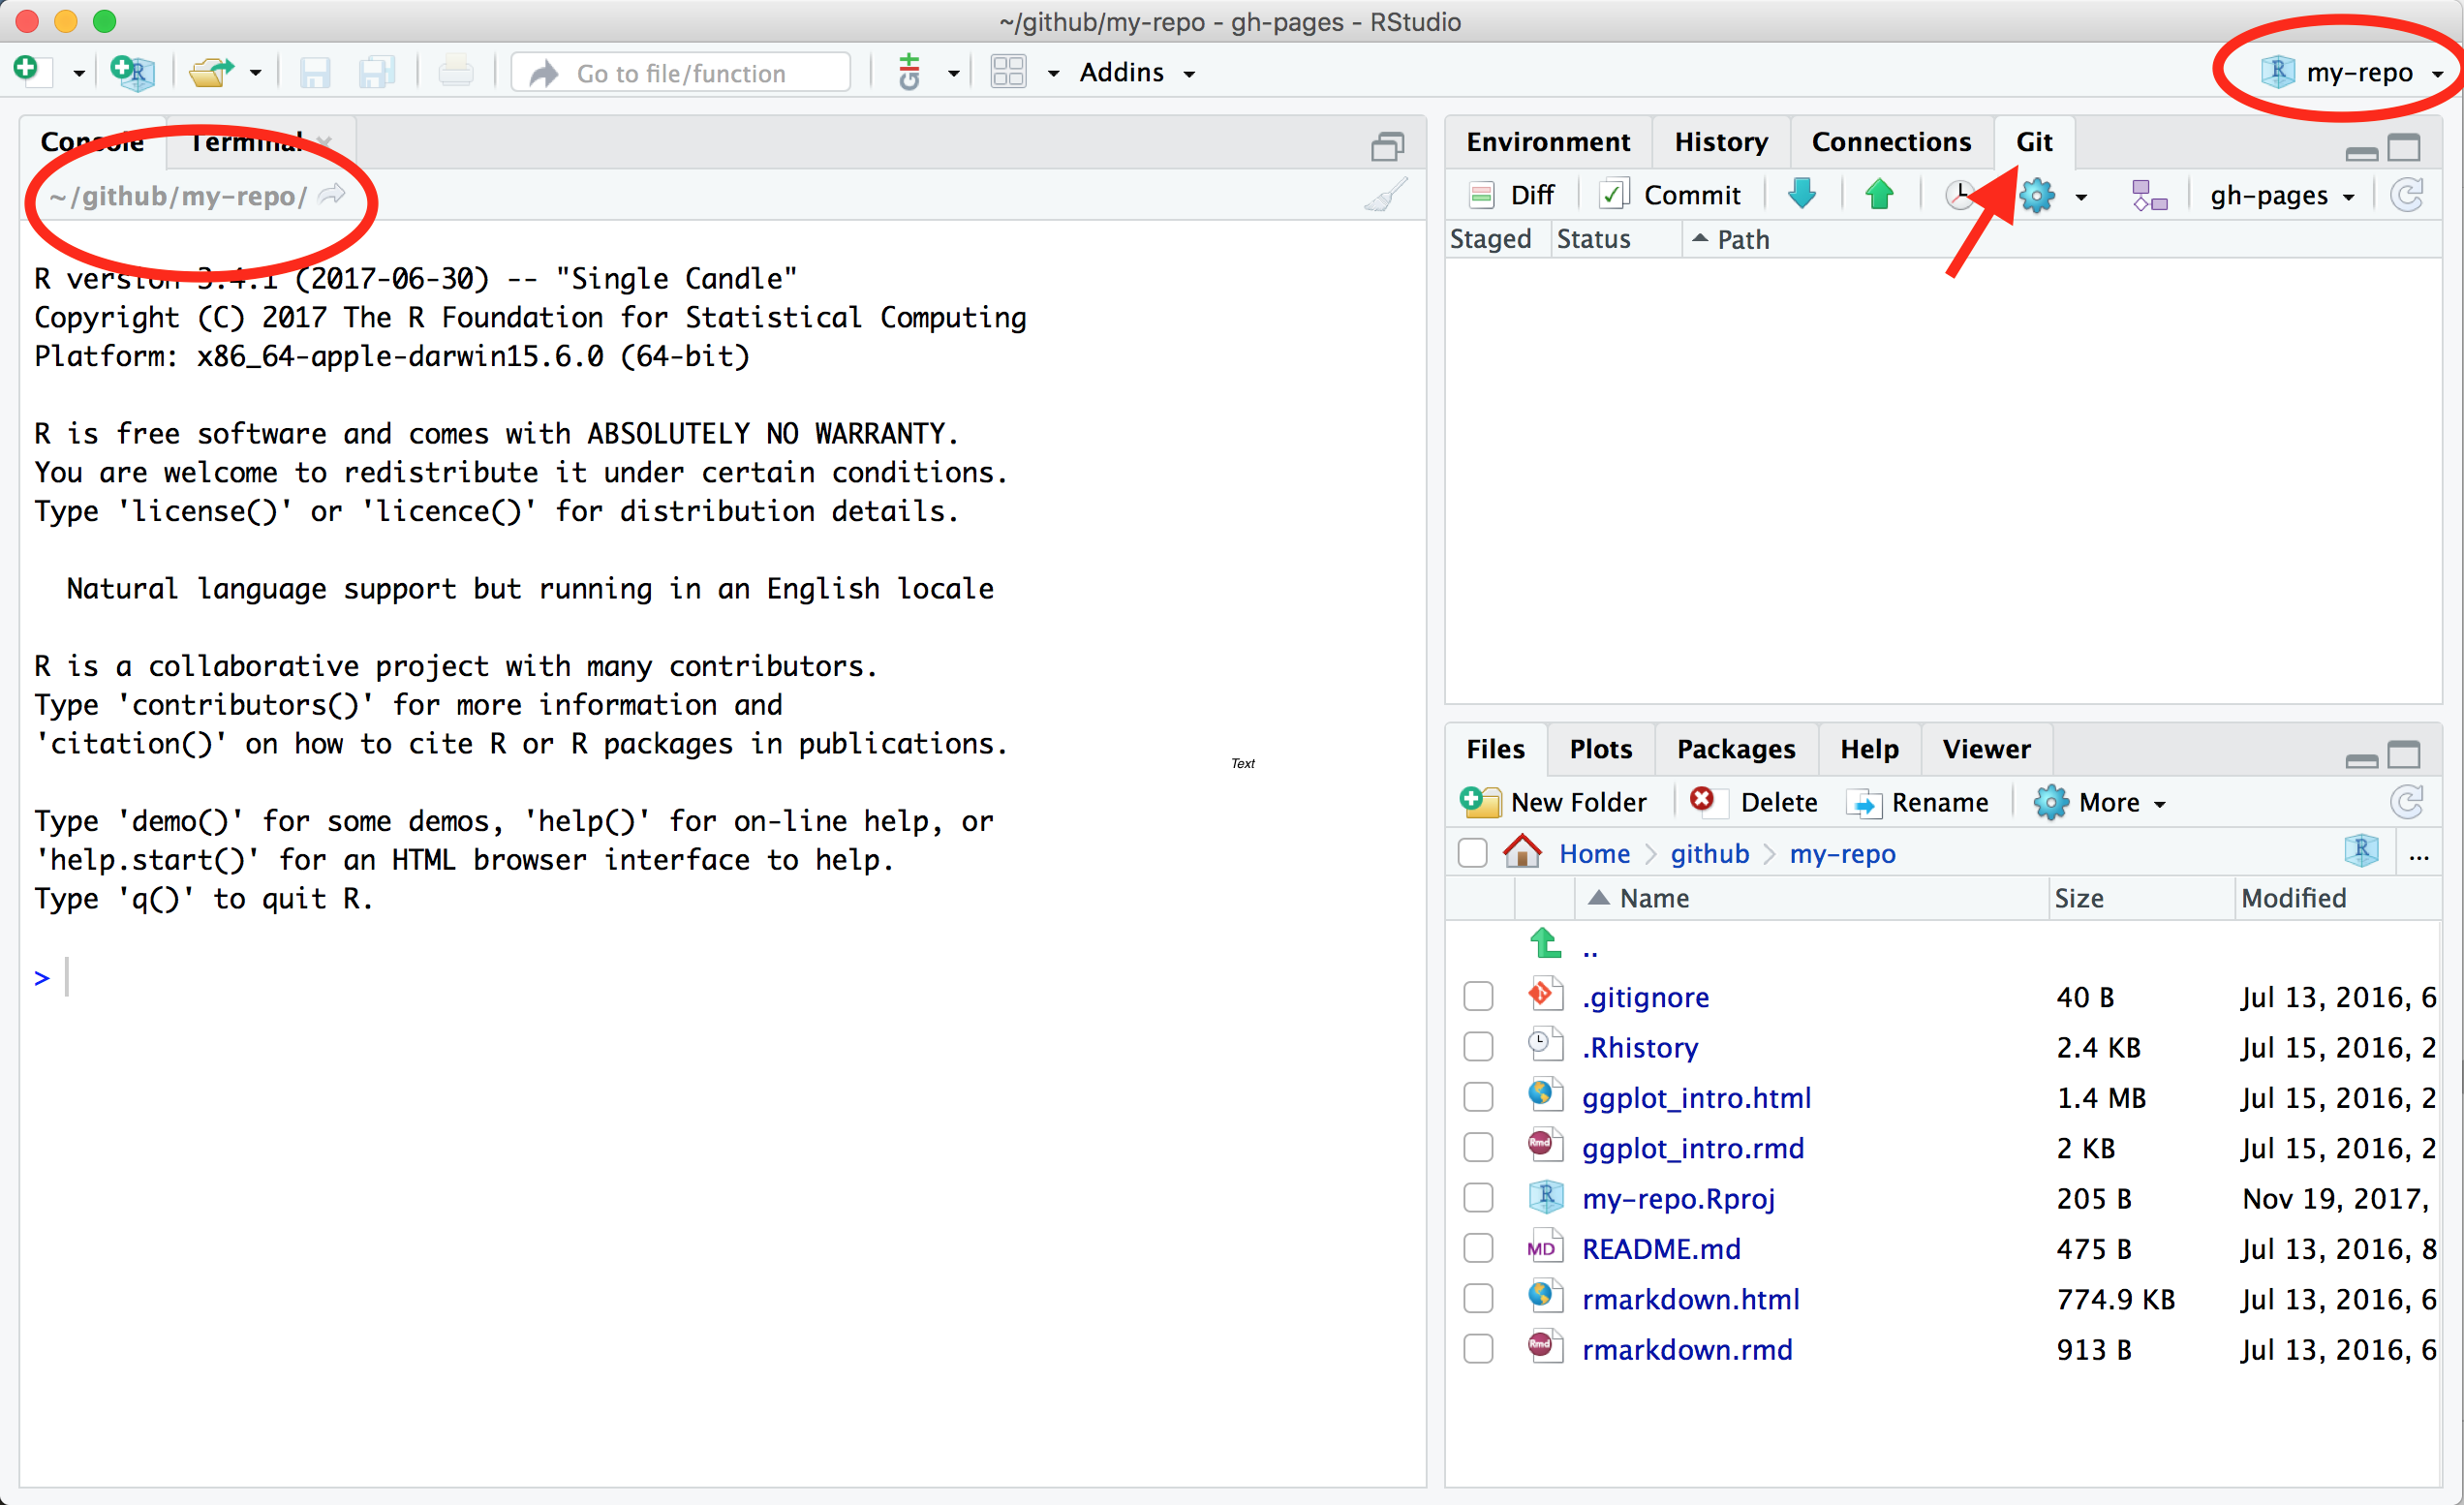
\includegraphics{img/RStudio_IDE_git.png}

When you first clone a repo through RStudio, RStudio will add an \texttt{.Rproj} file to your repo. And if you didn't add a \texttt{.gitignore} file when you originally created the repo on GitHub.com, RStudio will also add this for you. These will show up with little yellow \texttt{?} icons in your git tab. This is GitHub's way of saying: ``I am responsible for tracking everything that happens in this repo, but I haven't seen these files yet. Do you want me to track them too?'' (We'll see that when you click the box to stage them, they will turn into \texttt{A}s because they have been added to the repo.

\hypertarget{add-files-to-our-local-repo}{%
\section{Add files to our local repo}\label{add-files-to-our-local-repo}}

The repository will contain:

\begin{itemize}
\tightlist
\item
  .gitignore file
\item
  README.md
\item
  Rproj
\end{itemize}

Let's create the following:

\begin{itemize}
\tightlist
\item
  folder called ``data''
\item
  folder called ``figures''
\end{itemize}

They both show up in your Finder! \ldots{}

\hypertarget{get-data-files-into-your-working-directory}{%
\subsection{Get data files into your working directory}\label{get-data-files-into-your-working-directory}}

In Session 1, we introduced how and why R Projects are great for reproducibility, because our self-contained working directory will be the \textbf{first} place R looks for files.

You downloaded 7 files for this workshop, some comma separate value (CSV) files and some as Excel spreadsheets (.xlsx):

\begin{itemize}
\tightlist
\item
  fish\_counts\_curated.csv
\item
  invert\_counts\_curated.xlsx
\item
  kelp\_counts\_curated.xlsx
\item
  substrate\_cover\_curated.xlsx
\item
  lobster\_counts.xlsx
\item
  ca\_np.csv
\item
  ci\_np.xlsx
\end{itemize}

Copy and paste those files into the `data' subfolder of your R project. Notice that now these files are in your working directory when you go back to that Project in RStudio (check the `Files' tab and navigate to the data subfolder). That means they're going to be in the first place R will look when you ask it to find a file to read in.

I'm going to go to the Finder (Windows Explorer on a PC) and copy a file into my repository from there. And then I'm going to go back to RStudio -- it shows up in the git tab! So the repository is being tracked, no matter how you make changes to it (changes do not have to be done only through RStudio).

To make changes to the repository, you will work from your computer (``local Github'').

When files are changed in the local repository, these changes will be reflected in the Git tab of RStudio:

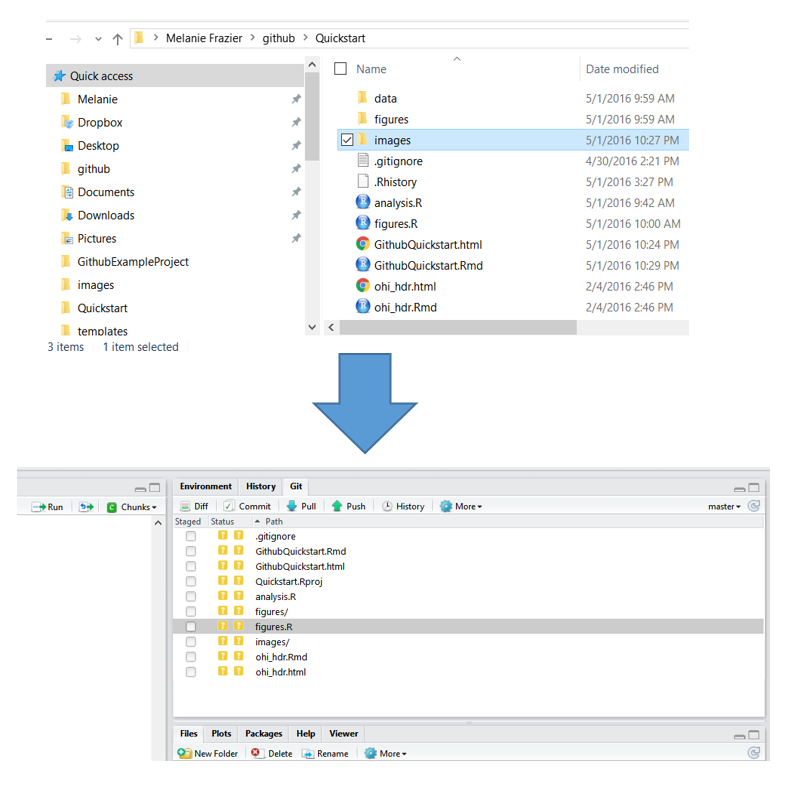
\includegraphics{img/modify_files.png}

\hypertarget{inspect-what-has-changed}{%
\subsection{Inspect what has changed}\label{inspect-what-has-changed}}

These are the codes RStudio uses to describe how the files are changed, (from the RStudio \href{http://www.rstudio.com/wp-content/uploads/2016/01/rstudio-IDE-cheatsheet.pdf}{cheatsheet}):
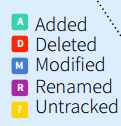
\includegraphics{img/modified.png}

\hypertarget{sync-from-rstudio-to-github}{%
\section{Sync from RStudio to GitHub}\label{sync-from-rstudio-to-github}}

When you are ready to commit your changes, you follow these steps:

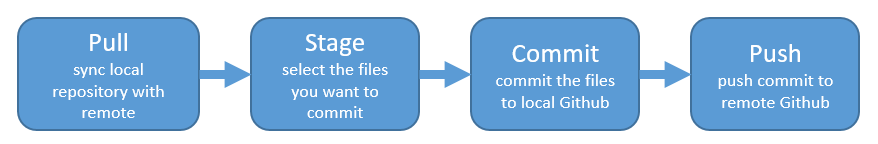
\includegraphics{img/commit_overview.png}

We walk through this process below:

\hypertarget{pull}{%
\subsection{Pull}\label{pull}}

From the Git tab, ``Pull'' the repository. This makes sure your local repository is synced with the remote repository. This is very important if other people are making changes to the repository or if you are working from multiple computers.

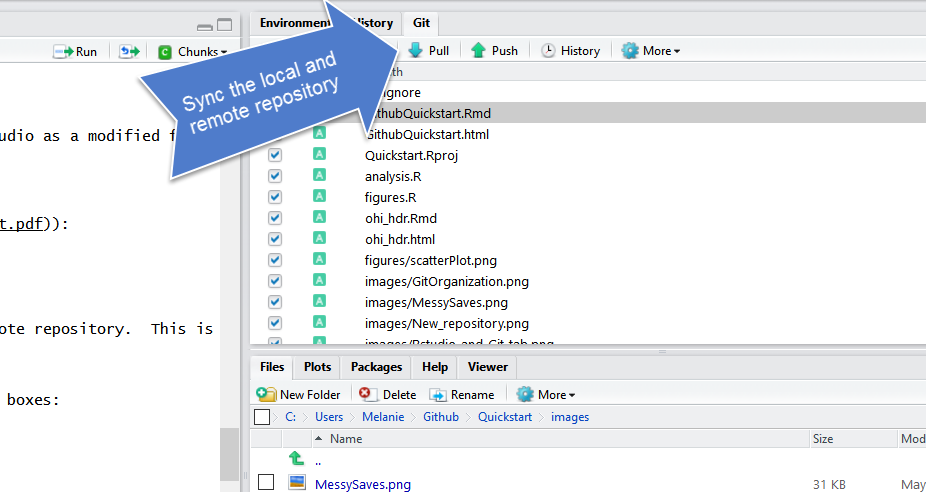
\includegraphics{img/pull.png}

\hypertarget{stage}{%
\subsection{Stage}\label{stage}}

Stage the files you want to commit. In RStudio, this involves checking the ``Staged'' boxes:

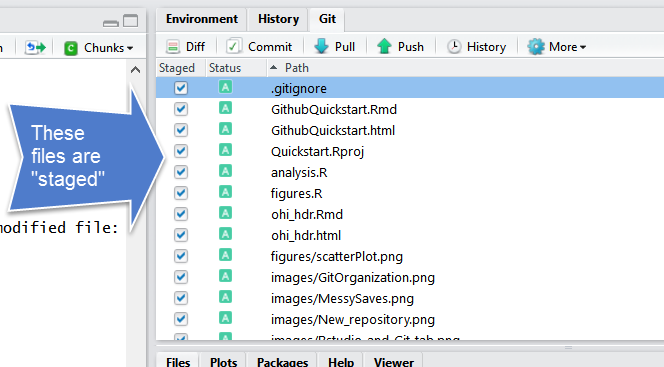
\includegraphics{img/staged.png}

\hypertarget{commit}{%
\subsection{Commit}\label{commit}}

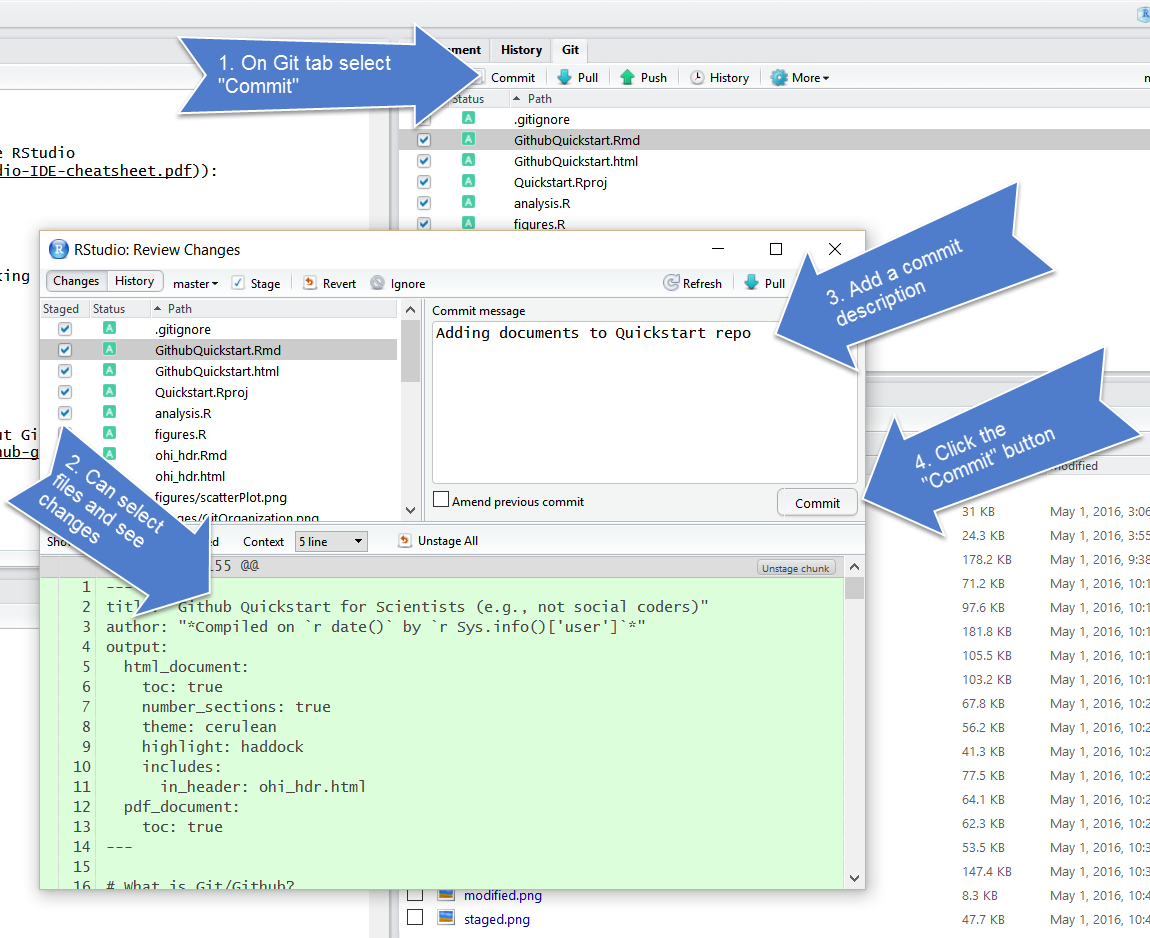
\includegraphics{img/commit.png}

\hypertarget{push}{%
\subsection{Push}\label{push}}

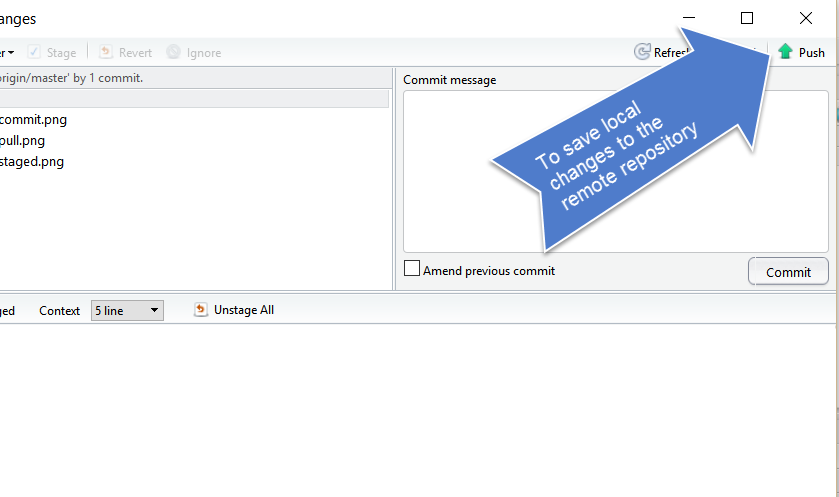
\includegraphics{img/push.png}

\hypertarget{explore-remote-github}{%
\section{Explore remote Github}\label{explore-remote-github}}

The files you added should be on github.com:

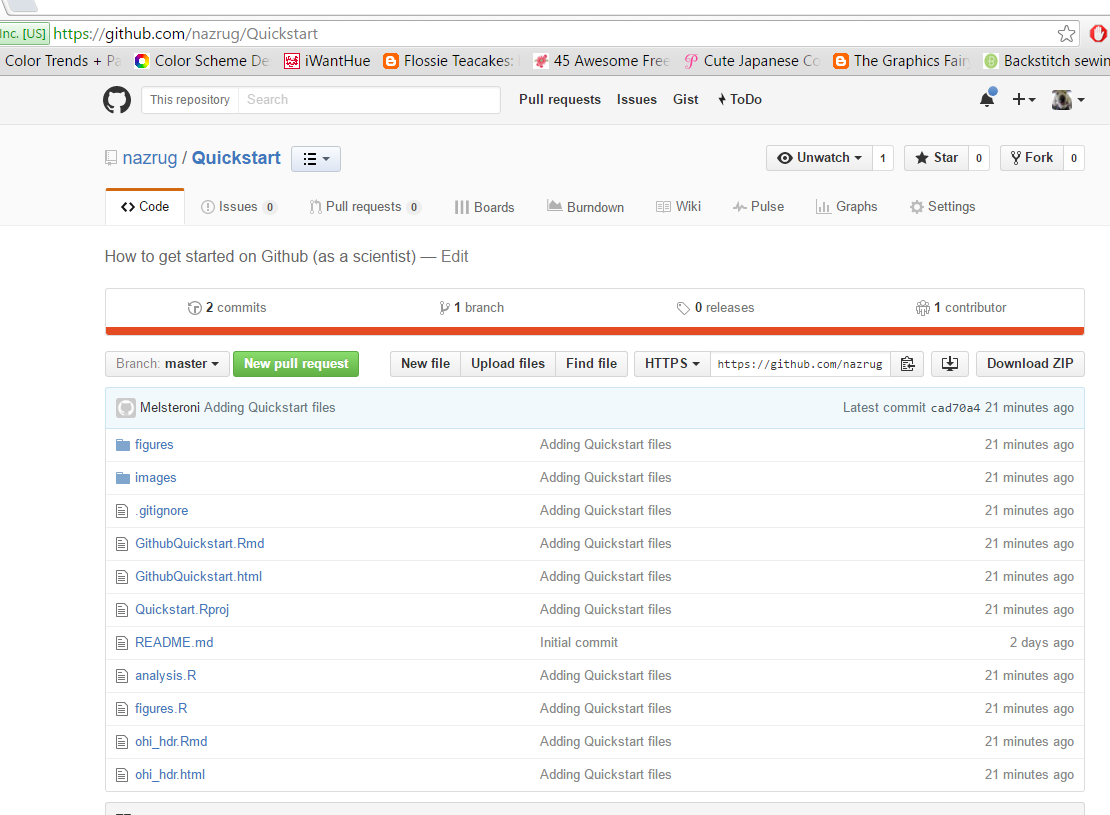
\includegraphics{img/Github_remote.png}

Let's also explore commit history, file history.

\hypertarget{activity-1}{%
\subsection{Activity}\label{activity-1}}

Go back to RStudio.

This time let's edit an existing file instead of adding something new. Open your README file by clicking on it in the Files pane (lower right corner). Write a few lines of text (like your dog's name), save, and see what happens in your Git Tab. Sync it to your remote repository at Github.com.

\hypertarget{create-a-new-r-markdown-file}{%
\section{Create a new R Markdown file}\label{create-a-new-r-markdown-file}}

Now get ourselves back into learning R. We are going to use R Markdown so that you can write notes to yourself in Markdown, and have a record of all your R code. Writing R commands in the console like we did this morning is great, but limited; it's hard to keep track of and hard to efficiently share with others. Plus, as your analyses get more complicated, you need to be able to see them all in one place.

Go to File \textgreater{} New File \textgreater{} R Markdown \ldots{} (or click the green plus in the top left corner).

Let's set up this file so we can use it for the rest of the day. I'm going to delete all the text that is already there and write some new text.

Here's what I'm going to write in my R Markdown file to begin:

\begin{verbatim}
---
title: "Reading data into R with `readxl`"
author: "Julie Lowndes"
date: "12/7/2019"
output: html_document
---

# Learning `readxl`

We are working with data and it's going to be amazing.
\end{verbatim}

Now, let's save it. I'm going to call my file \texttt{readxl.Rmd}. You can knit it if you'd like.

Then, knit your file, and sync your file to GitHub: commit and pull

What if a file doesn't show up in the Git tab and you expect that it should? Check to make sure you've saved the file. If the filename is red with an asterix, there have been changes since it was saved. Remember to save before syncing to GitHub!

\hypertarget{explore-your-webpage}{%
\section{Explore your webpage}\label{explore-your-webpage}}

You've just created a webpage!

It will exist at this url: username.github.io/repo-name/filename. Mine is: jules32.github.io/r-workshop/readxl.

Troubleshooting:

\begin{itemize}
\tightlist
\item
  404 error? Remove trailing / from the url
\item
  Wants you to download? Remove trailing .Rmd from the url
\end{itemize}

\hypertarget{committing---how-often-tracking-changes-in-your-files}{%
\section{Committing - how often? Tracking changes in your files}\label{committing---how-often-tracking-changes-in-your-files}}

Whenever you make changes to the files in Github, you will walk through the Pull -\textgreater{} Stage -\textgreater{} Commit -\textgreater{} Push steps.

I tend to do this every time I finish a task (basically when I start getting nervous that I will lose my work). Once something is committed, it is very difficult to lose it.

One thing that I love about about Github is that it is easy to see how files have changed over time. Usually I compare commits through github.com:

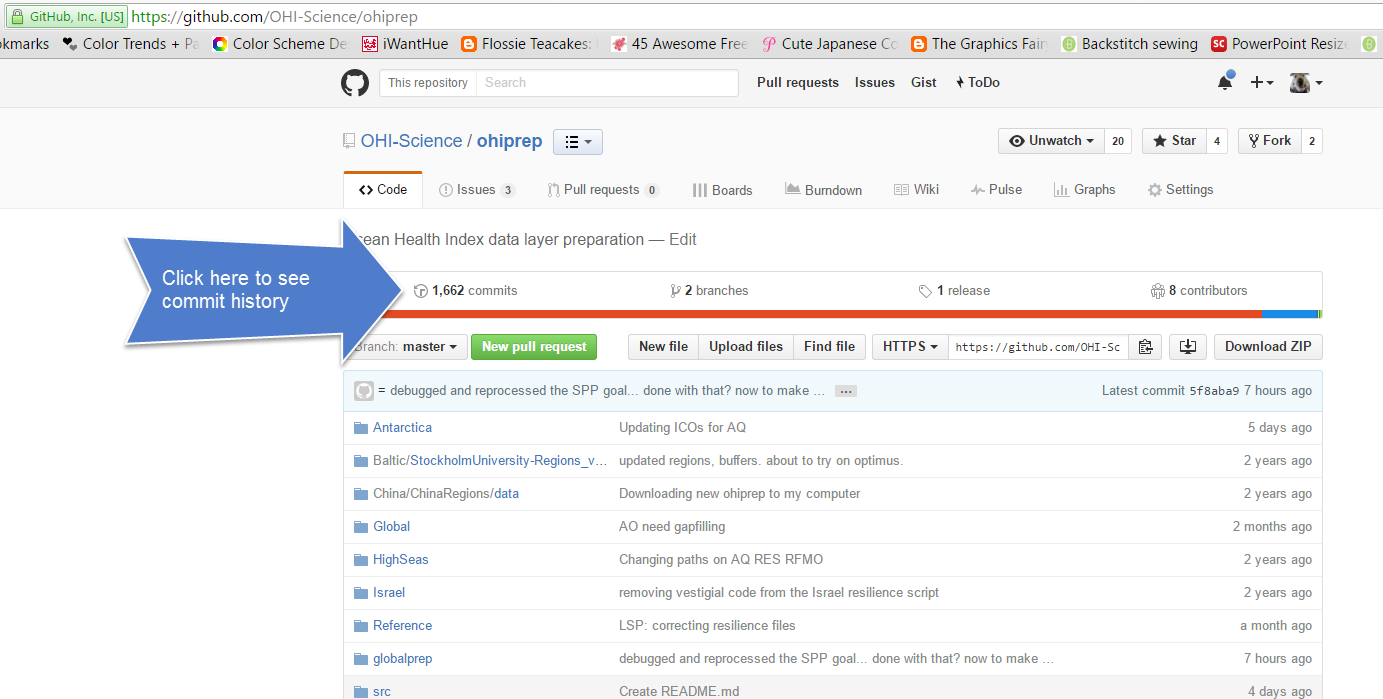
\includegraphics{img/commit_history.png}

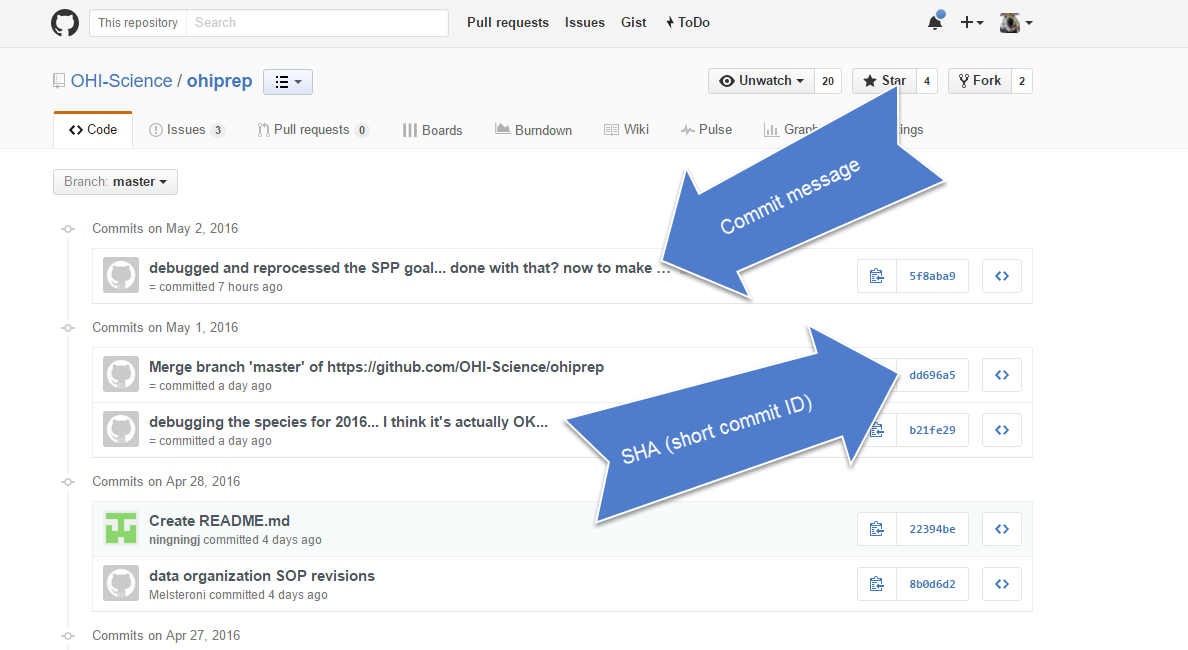
\includegraphics{img/commit_compare_2.png}

You can click on the commits to see how the files changed from the previous commit:

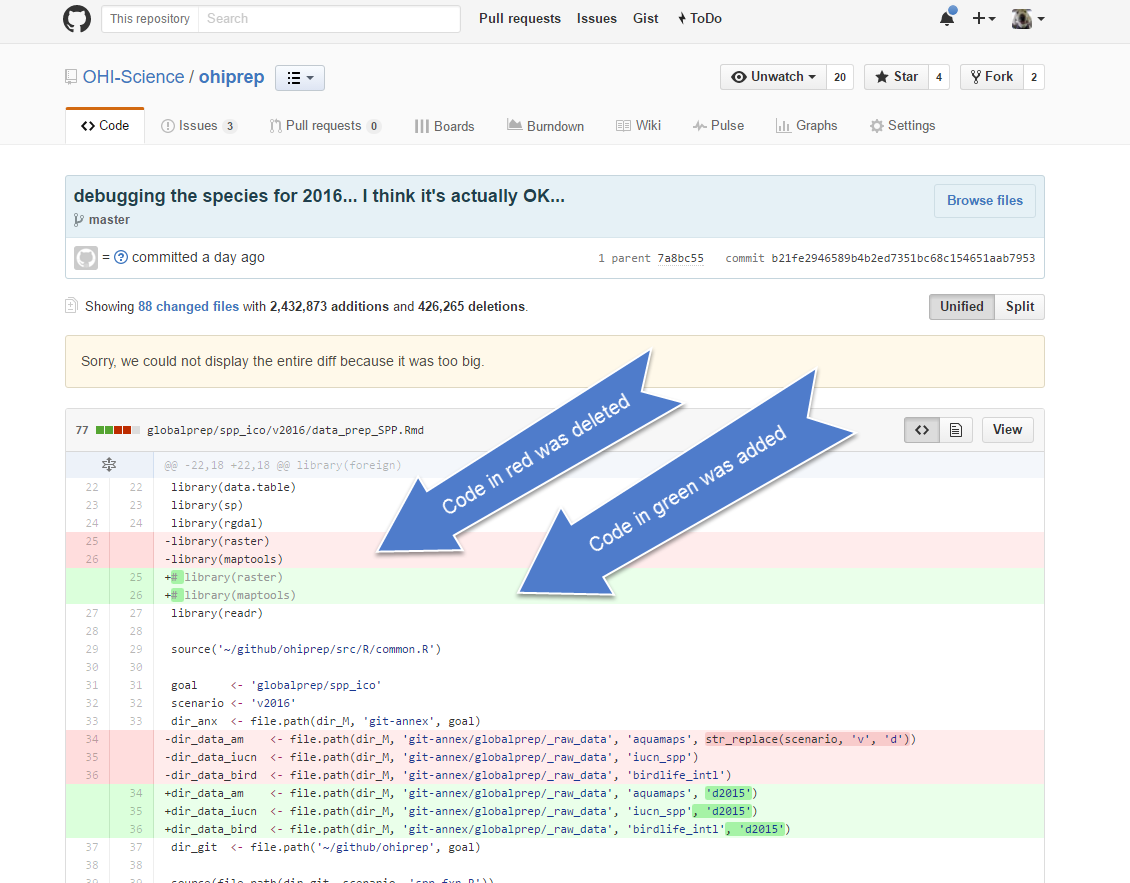
\includegraphics{img/commit_compare_3.png}

\hypertarget{happy-git-with-r}{%
\section{Happy Git with R}\label{happy-git-with-r}}

If you have problems, we'll help you out using Jenny Bryan's \href{http://happygitwithr.com}{HappyGitWithR}, particularly the sections on \href{http://happygitwithr.com/rstudio-see-git.html}{Detect Git from RStudio} and \href{http://happygitwithr.com/troubleshooting.html}{RStudio, Git, GitHub Hell (troubleshooting)}. So as we are coming around, have a look at it and see if you can help troubleshoot too!

\hypertarget{efficiency-tips-1}{%
\section{Efficiency Tips}\label{efficiency-tips-1}}

\hypertarget{readxl}{%
\chapter{\texorpdfstring{\texttt{readxl}}{readxl}}\label{readxl}}

\hypertarget{summary-2}{%
\section{Summary}\label{summary-2}}

\textbf{Check this, may need to be a block quote}: The \textbf{readxl} package makes it easy to import tabular data from Excel spreadsheets (.xls or .xlsx files) and includes several options for cleaning data during import. \textbf{readxl} has no external dependencies and functions on any operating system, making it an OS- and user-friendly package that simplifies getting your data from Excel into R.

\hypertarget{objectives-2}{%
\subsection{Objectives}\label{objectives-2}}

\begin{itemize}
\tightlist
\item
  Use \texttt{read\_csv()} to read in a comma separated value (CSV) file
\item
  Use \texttt{read\_excel()} to read in an Excel worksheet from a workbook
\item
  Replace a specific string/value in a spreadsheet with with \texttt{NA}
\item
  Skip \emph{n} rows when importing an Excel worksheet
\item
  Use \texttt{read\_excel()} to read in parts of a worksheet (by cell range)
\item
  Specify column names when importing Excel data
\item
  Read and combine data from multiple Excel worksheets into a single df using \texttt{purrr::map\_df()}
\item
  Write data using \texttt{write\_csv()} or \texttt{write\_xlsx()}
\item
  Workflows with \texttt{readxl}: considerations, limitations, reproducibility
\end{itemize}

\hypertarget{resources-3}{%
\subsection{Resources}\label{resources-3}}

\begin{itemize}
\tightlist
\item
  \url{https://readxl.tidyverse.org/}
\item
  \href{https://readxl.tidyverse.org/articles/articles/readxl-workflows.html}{readxl Workflows article (from tidyverse.org)}
\end{itemize}

\hypertarget{lesson}{%
\section{Lesson}\label{lesson}}

\hypertarget{attach-packages}{%
\subsection{Attach packages}\label{attach-packages}}

In the .Rmd you just created, attach the \texttt{tidyverse}, \texttt{readxl}, \texttt{writexl}, and \texttt{here} packages

In this lesson, we'll read in a CSV file with the \texttt{read\_csv()} function, so we need to have the \texttt{readr} package attached. Since it's part of the \texttt{tidyverse}, we'll go ahead and attach the \texttt{tidyverse} package below our script header using \texttt{library(package\_name)}. It's a good idea to attach packages within the set-up chunk in R Markdown, so we'll also attach the \texttt{readxl}, \texttt{writexl}, and \texttt{here} packages there.

Here's our first code chunk:

\begin{verbatim}
{r setup, eval = FALSE}
knitr::opts_chunk$set(echo = TRUE)

# Attach the tidyverse, readxl, writexl and here packages:
library(tidyverse)
library(readxl)
library(writexl)
library(here)
\end{verbatim}

Now, all of the packages and functions within the \texttt{tidyverse} and \texttt{readxl}, including \texttt{read\_csv()} and \texttt{read\_excel()}, are available for use.

\hypertarget{use-read_csv-to-read-in-data-from-a-csv-file}{%
\subsection{\texorpdfstring{Use \texttt{read\_csv()} to read in data from a CSV file}{Use read\_csv() to read in data from a CSV file}}\label{use-read_csv-to-read-in-data-from-a-csv-file}}

There are many types of files containing data that you might want to work with in R. A common one is a comma separated value (CSV) file, which contains values with each column entry separated by a comma delimiter. CSVs can be opened, viewed, and worked with in Excel just like an .xls or .xlsx file - but let's learn how to get data directly from a CSV into R where we can work with it more reproducibly.

The CSV we'll read in here is called ``fish\_counts\_curated.csv'', and contains observations for ``the abundance and size of fish species as part of SBCLTER's kelp forest monitoring program to track long-term patterns in species abundance and diversity'' from the \href{http://sbc.lternet.edu/}{Santa Barbara Channel Long Term Ecological Research} program.

\textbf{Source:} Reed D. 2018. SBC LTER: Reef: Kelp Forest Community Dynamics: Fish abundance. Environmental Data Initiative. \url{https://doi.org/10.6073/pasta/dbd1d5f0b225d903371ce89b09ee7379}. Dataset accessed 9/26/2019.

Read in the ``fish\_counts\_curated.csv'' file \texttt{read\_csv("file\_name.csv")}, and store it in R as an object called \emph{fish\_counts}:

\begin{Shaded}
\begin{Highlighting}[]
\NormalTok{fish_counts <-}\StringTok{ }\KeywordTok{read_csv}\NormalTok{(}\KeywordTok{here}\NormalTok{(}\StringTok{"data"}\NormalTok{, }\StringTok{"fish_counts_curated.csv"}\NormalTok{))}
\end{Highlighting}
\end{Shaded}

Notice that the name of the stored object (here, \emph{fish\_counts}) will show up in our Environment tab in RStudio.

Click on the object in the Environment, and R will automatically run the \texttt{View()} function for you to pull up your data in a separate viewing tab. Now we can look at it in the spreadsheet format we're used to.

Here are a few other functions for quickly exploring imported data:

\begin{itemize}
\tightlist
\item
  \texttt{summary()}: summary of class, dimensions, \texttt{NA} values, etc.
\item
  \texttt{names()}: variable names (column headers)
\item
  \texttt{ls()}: list all objects in environment
\item
  \texttt{head()}: Show the first x rows (default is 6 lines)
\item
  \texttt{tail()}: Show the last x rows (default is 6 lines)
\end{itemize}

Now that we have our fish counts data ready to work with in R, let's get the substrate cover and kelp data (both .xlsx files). In the following sections, we'll learn that we can use \texttt{read\_excel()} to read in Excel files directly.

\hypertarget{use-read_excel-to-read-in-a-single-excel-worksheet}{%
\subsection{\texorpdfstring{Use \texttt{read\_excel()} to read in a single Excel worksheet}{Use read\_excel() to read in a single Excel worksheet}}\label{use-read_excel-to-read-in-a-single-excel-worksheet}}

First, take a look at \emph{substrate\_cover\_curated.xlsx} in Excel, which contains a single worksheet with substrate type and percent cover observations at different sampling locations in the Santa Barbara Channel.

A few things to notice:

\begin{itemize}
\tightlist
\item
  The file contains a single worksheet
\item
  There are multiple rows containing text information up top
\item
  Where observations were not recorded, there exists `-9999'
\end{itemize}

Let's go ahead and read in the data. If the file is in our working directory, we can read in a single worksheet .xlsx file using \texttt{read\_excel("file\_name.xlsx")}. \emph{Note: read\_excel() works for both .xlsx and .xls types}.

Like this:

\begin{Shaded}
\begin{Highlighting}[]
\NormalTok{substrate_cover <-}\StringTok{ }\KeywordTok{read_excel}\NormalTok{(}\KeywordTok{here}\NormalTok{(}\StringTok{"data"}\NormalTok{, }\StringTok{"substrate_cover_curated.xlsx"}\NormalTok{))}
\end{Highlighting}
\end{Shaded}

\textbf{Tada? Not quite.}

Click on the object name (\emph{substrate\_cover}) in the Environment to view the data in a new tab. A few things aren't ideal:

\begin{Shaded}
\begin{Highlighting}[]
\NormalTok{substrate_cover}
\end{Highlighting}
\end{Shaded}

\begin{verbatim}
## # A tibble: 23,942 x 9
##    `Substrate cover dataset,~ ...2  ...3   ...4  ...5  ...6  ...7  ...8   ...9  
##    <chr>                      <chr> <chr>  <chr> <chr> <chr> <chr> <chr>  <chr> 
##  1 Source: https://portal.ed~ <NA>  <NA>   <NA>  <NA>  <NA>  <NA>  <NA>   <NA>  
##  2 Accessed: 9/28/2019        <NA>  <NA>   <NA>  <NA>  <NA>  <NA>  <NA>   <NA>  
##  3 <NA>                       <NA>  <NA>   <NA>  <NA>  <NA>  <NA>  <NA>   <NA>  
##  4 year                       month date   site  tran~ quad  side  subst~ perce~
##  5 -9999                      -9999 -9999  carp  1     20    i     b      -9999 
##  6 2000                       9     -9999  carp  1     20    o     b      -9999 
##  7 2000                       9     9/8/00 carp  1     20    i     b      100   
##  8 2000                       9     9/8/00 carp  1     20    o     b      100   
##  9 2000                       9     9/8/00 carp  1     40    i     b      100   
## 10 2000                       9     9/8/00 carp  1     40    o     b      100   
## # ... with 23,932 more rows
\end{verbatim}

\begin{itemize}
\tightlist
\item
  The top row of text has automatically become the (messy) column headers
\item
  There are multiple descriptive rows before we actually get to the data
\item
  There are -9999s that we want R to understand \texttt{NA} instead
\end{itemize}

We can deal with those issues by adding arguments within \texttt{read\_excel()}. Include argument \texttt{skip\ =\ n} to skip the first `n' rows when importing data, and \texttt{na\ =\ "this"} to replace ``this'' with \texttt{NA} when importing:

\begin{Shaded}
\begin{Highlighting}[]
\NormalTok{substrate_cover <-}\StringTok{ }\KeywordTok{read_excel}\NormalTok{(}\KeywordTok{here}\NormalTok{(}\StringTok{"data"}\NormalTok{, }\StringTok{"substrate_cover_curated.xlsx, skip = 4, na = "}\OperatorTok{-}\DecValTok{9999}\StringTok{")}
\end{Highlighting}
\end{Shaded}

\begin{Shaded}
\begin{Highlighting}[]
\NormalTok{substrate_cover}
\end{Highlighting}
\end{Shaded}

\begin{verbatim}
## # A tibble: 23,938 x 9
##    year  month date   site  transect quad  side  substrate_type percent_cover
##    <chr> <chr> <chr>  <chr> <chr>    <chr> <chr> <chr>          <chr>        
##  1 <NA>  <NA>  <NA>   carp  1        20    i     b              <NA>         
##  2 2000  9     <NA>   carp  1        20    o     b              <NA>         
##  3 2000  9     9/8/00 carp  1        20    i     b              100          
##  4 2000  9     9/8/00 carp  1        20    o     b              100          
##  5 2000  9     9/8/00 carp  1        40    i     b              100          
##  6 2000  9     9/8/00 carp  1        40    o     b              100          
##  7 2000  9     9/8/00 carp  2        20    i     b              90           
##  8 2000  9     9/8/00 carp  2        20    o     b              80           
##  9 2000  9     9/8/00 carp  2        40    i     b              80           
## 10 2000  9     9/8/00 carp  2        40    o     b              85           
## # ... with 23,928 more rows
\end{verbatim}

Check out \emph{substrate\_cover}, and see that the first row \emph{after} the 4 skipped are the column names, and all -9999s have been updated to \texttt{NA}. Hooray!

\hypertarget{use-read_excel-to-read-in-only-part-of-an-excel-worksheet}{%
\subsection{\texorpdfstring{Use \texttt{read\_excel()} to read in only \emph{part} of an Excel worksheet}{Use read\_excel() to read in only part of an Excel worksheet}}\label{use-read_excel-to-read-in-only-part-of-an-excel-worksheet}}

We always advocate for leaving the raw data raw, and writing a complete script containing all steps of data wrangling \& transformation. But in \emph{some} situations (be careful), you may want to specify a range of cells to read in from an Excel worksheet.

You can specify a range of cells to read in using the \texttt{range\ =} argument in \texttt{read\_excel()}. For example, if I want to read in the rectangle from D12:I15 in \emph{substrate\_cover\_curated.xlsx} - only observations for Carpenteria Beach (Transect 2) in September 2000 - I can use:

\begin{Shaded}
\begin{Highlighting}[]
\NormalTok{carp_cover_}\DecValTok{2000}\NormalTok{ <-}\StringTok{ }\KeywordTok{read_excel}\NormalTok{(}\KeywordTok{here}\NormalTok{(}\StringTok{"data"}\NormalTok{, }\StringTok{"substrate_cover_curated.xlsx"}\NormalTok{, }\DataTypeTok{range =} \StringTok{"D12:I15"}\NormalTok{)}
\end{Highlighting}
\end{Shaded}

But yuck. Look at \emph{carp\_cover\_2000} and you'll notice that the first row \emph{of that range} is automatically made the column headers. To keep all rows within a range and \textbf{add your own column names}, add a \texttt{col\_names\ =} argument:

\begin{Shaded}
\begin{Highlighting}[]
\NormalTok{carp_cover_}\DecValTok{2000}\NormalTok{ <-}\StringTok{ }\KeywordTok{read_excel}\NormalTok{(}\KeywordTok{here}\NormalTok{(}\StringTok{"data"}\NormalTok{, }\StringTok{"substrate_cover_curated.xlsx"}\NormalTok{, }\DataTypeTok{range =} \StringTok{"D12:I15"}\NormalTok{, }\DataTypeTok{col_names =} \KeywordTok{c}\NormalTok{(}\StringTok{"site_name"}\NormalTok{, }\StringTok{"transect"}\NormalTok{, }\StringTok{"quad"}\NormalTok{, }\StringTok{"plot_side"}\NormalTok{, }\StringTok{"type"}\NormalTok{, }\StringTok{"coverage"}\NormalTok{))}
\end{Highlighting}
\end{Shaded}

\begin{Shaded}
\begin{Highlighting}[]
\NormalTok{carp_cover_}\DecValTok{2000}
\end{Highlighting}
\end{Shaded}

\begin{verbatim}
## # A tibble: 4 x 6
##   site_name transect quad  plot_side type  coverage
##   <chr>     <chr>    <chr> <chr>     <chr> <chr>   
## 1 carp      2        20    i         b     90      
## 2 carp      2        20    o         b     80      
## 3 carp      2        40    i         b     80      
## 4 carp      2        40    o         b     85
\end{verbatim}

So far we've read in a single CSV file using \texttt{read\_csv()}, and an Excel file containing a single worksheet with \texttt{read\_excel()}. Now let's read in data from an Excel workbook with multiple worksheets.

\hypertarget{use-read_excel-to-read-in-selected-worksheets-from-a-workbook}{%
\subsection{\texorpdfstring{Use \texttt{read\_excel()} to read in selected worksheets from a workbook}{Use read\_excel() to read in selected worksheets from a workbook}}\label{use-read_excel-to-read-in-selected-worksheets-from-a-workbook}}

Now, we'll read in the kelp fronds data from file \emph{kelp\_counts\_curated.xlsx}. If you open the Excel workbook, you'll see that it contains multiple worksheets with giant kelp observations in the Santa Barbara Channel during July 2016, 2017, and 2018, with data collected at each \emph{site} in a separate worksheet.

To read in a single Excel worksheet from a workbook we'll again use \texttt{read\_excel("file\_name.xlsx")}, but we'll need to let R know which worksheet to get.

Let's read in the kelp data just like we did above, as an object called \emph{kelp\_counts}.

\begin{Shaded}
\begin{Highlighting}[]
\NormalTok{kelp_counts <-}\StringTok{ }\KeywordTok{read_excel}\NormalTok{(}\KeywordTok{here}\NormalTok{(}\StringTok{"data"}\NormalTok{, }\StringTok{"kelp_counts_curated.xlsx"}\NormalTok{)}
\end{Highlighting}
\end{Shaded}

You might be thinking, ``Hooray, I got all of my Excel workbook data!'' But remember to always look at your data - you will see that actually only the first worksheet was read in. The default in \texttt{read\_excel()} is to read in the \textbf{first worksheet} in a multi-sheet Excel workbook.

To check the worksheet names in an Excel workbook, use \texttt{excel\_sheets()}:

\begin{Shaded}
\begin{Highlighting}[]
\KeywordTok{excel_sheets}\NormalTok{(}\KeywordTok{here}\NormalTok{(}\StringTok{"data"}\NormalTok{, }\StringTok{"kelp_counts_curated.xlsx"}\NormalTok{)}
\end{Highlighting}
\end{Shaded}

If we want to read in data from a worksheet other than the first one in an Excel workbook, we can specify the correct worksheet by name or position by adding the \texttt{sheet} argument.

Let's read in data from the worksheet named \emph{golb} (Goleta Beach) in the \emph{kelp\_counts\_curated.xlsx} workbook:

\begin{Shaded}
\begin{Highlighting}[]
\NormalTok{kelp_golb <-}\StringTok{ }\KeywordTok{read_excel}\NormalTok{(}\KeywordTok{here}\NormalTok{(}\StringTok{"data"}\NormalTok{, }\StringTok{"kelp_counts_curated.xlsx"}\NormalTok{, }\DataTypeTok{sheet =} \StringTok{"golb"}\NormalTok{))}
\end{Highlighting}
\end{Shaded}

Note that you can also specify a worksheet by position: since \emph{golb} is the 6\textsuperscript{th} worksheet in the workbook, we could also use the following:

\begin{Shaded}
\begin{Highlighting}[]
\NormalTok{kelp_golb <-}\StringTok{ }\KeywordTok{read_excel}\NormalTok{(}\KeywordTok{here}\NormalTok{(}\StringTok{"data"}\NormalTok{, }\StringTok{"kelp_counts_curated.xlsx"}\NormalTok{, }\DataTypeTok{sheet =} \DecValTok{6}\NormalTok{))}
\end{Highlighting}
\end{Shaded}

\begin{Shaded}
\begin{Highlighting}[]
\NormalTok{kelp_golb}
\end{Highlighting}
\end{Shaded}

\begin{verbatim}
## # A tibble: 3 x 4
##   year  month site  total_fronds
##   <chr> <chr> <chr>        <dbl>
## 1 2016  7     golb          2557
## 2 2017  7     golb          1575
## 3 2018  7     golb          1629
\end{verbatim}

\hypertarget{read-in-and-combine-data-from-multiple-worksheets-into-a-data-frame-simultaneously-with-purrrmap_df}{%
\subsection{\texorpdfstring{Read in and combine data from multiple worksheets into a data frame simultaneously with \texttt{purrr::map\_df()}}{Read in and combine data from multiple worksheets into a data frame simultaneously with purrr::map\_df()}}\label{read-in-and-combine-data-from-multiple-worksheets-into-a-data-frame-simultaneously-with-purrrmap_df}}

So far, we've read in entire Excel worksheets and pieces of a worksheet. What if we have a workbook (like \emph{kelp\_counts\_curated.xlsx}) that contains worksheets that contain observations for the same variables, in the same organization? Then we may want to read in data from \emph{all} worksheets, and combine them into a single data frame.

We'll use \texttt{purrr::map\_df()} to loop through all the worksheets in a workbook, reading them in \& putting them together into a single df in the process.

The steps we'll go through in the code below are:

\begin{itemize}
\tightlist
\item
  Set a pathway so that R knows where to look for an Excel workbook
\item
  Get the names of all worksheets in that workbook with \texttt{excel\_sheets()}
\item
  Set names of a vector with \texttt{set\_names()}
\item
  Read in all worksheets, and put them together into a single data frame with \texttt{purrr::map\_df()}
\end{itemize}

\textbf{QUESTION: TODO Have they learned the pipe operator at this point?}

\textbf{Expect the question:} Why do I need to use read\_excel() instead of just giving it the file path (as below)?

\begin{Shaded}
\begin{Highlighting}[]
\NormalTok{kelp_path <-}\StringTok{ }\KeywordTok{here}\NormalTok{(}\StringTok{"data"}\NormalTok{, }\StringTok{"kelp_counts_curated.xlsx"}\NormalTok{)}

\NormalTok{kelp_all_sites <-}\StringTok{ }\NormalTok{kelp_path }\OperatorTok\StringTok{ }
\StringTok{  }\KeywordTok{excel_sheets}\NormalTok{() }\OperatorTok\StringTok{ }
\StringTok{  }\KeywordTok{set_names}\NormalTok{() }\OperatorTok\StringTok{ }
\StringTok{  }\NormalTok{purrr}\OperatorTok{::}\KeywordTok{map_df}\NormalTok{(read_excel, kelp_path)}
\end{Highlighting}
\end{Shaded}

Check out \emph{kelp\_all\_sites}, and notice that now the data from all 11 sites is now collected into a single data frame:

\begin{Shaded}
\begin{Highlighting}[]
\NormalTok{kelp_all_sites}
\end{Highlighting}
\end{Shaded}

\begin{verbatim}
## # A tibble: 32 x 4
##    year  month site  total_fronds
##    <chr> <chr> <chr>        <dbl>
##  1 2016  7     abur           307
##  2 2017  7     abur           604
##  3 2018  7     abur          3532
##  4 2016  7     ahnd          2572
##  5 2017  7     ahnd            16
##  6 2018  7     ahnd            16
##  7 2016  7     aque         11152
##  8 2017  7     aque          9194
##  9 2018  7     aque          7754
## 10 2016  7     bull          6706
## # ... with 22 more rows
\end{verbatim}

\hypertarget{save-data-frames-as-.csv-or-.xlsx-with-write_csv-or-write_xlsx}{%
\subsection{\texorpdfstring{Save data frames as .csv or .xlsx with \texttt{write\_csv()} or \texttt{write\_xlsx()}}{Save data frames as .csv or .xlsx with write\_csv() or write\_xlsx()}}\label{save-data-frames-as-.csv-or-.xlsx-with-write_csv-or-write_xlsx}}

There are a number of reasons you might want to save (/export) data in a data frame as a .csv or Excel worksheet, including:

\begin{itemize}
\tightlist
\item
  To store raw data within the project you're working in
\item
  To store copies of intermediate data frames
\item
  To convert your data back to a format that your coworkers/clients/colleagues will be able to use it more easily
\end{itemize}

Use \texttt{write\_csv(object,\ "file\_name.csv")} to write a data frame to a CSV, or \texttt{write\_xlsx(object,\ "file\_name.xlsx")} to similarly export as a .xlsx (or .xls) worksheet.

In the previous step, we combined all of our kelp frond observations into a single data frame. Wouldn't it make sense to store a copy?

As a CSV:

\begin{Shaded}
\begin{Highlighting}[]
\KeywordTok{write_csv}\NormalTok{(kelp_all_sites, }\KeywordTok{here}\NormalTok{(}\StringTok{"data"}\NormalTok{, }\StringTok{"kelp_all_sites.csv"}\NormalTok{))}
\end{Highlighting}
\end{Shaded}

A cool thing about \texttt{write\_csv()} is that it just quietly \emph{works} without wrecking anything else you do in a sequence, so it's great to add at the end of a piped sequence.

For example, if I want to read in the `ivee' worksheet from kelp\_counts\_curated.xlsx, select only columns `year' and `total\_fronds', then write that new subset to a .csv file, I can pipe all the way through:

\begin{Shaded}
\begin{Highlighting}[]
\NormalTok{kelp_ivee <-}\StringTok{ }\KeywordTok{read_excel}\NormalTok{(}\StringTok{"kelp_counts_curated.xlsx"}\NormalTok{, }\DataTypeTok{sheet =} \StringTok{"ivee"}\NormalTok{) }\OperatorTok\StringTok{ }
\StringTok{  }\CommentTok{#select(year, total_fronds) %>%  }\AlertTok{TODO}\CommentTok{: change this to read in a range}
\StringTok{  }\KeywordTok{write_csv}\NormalTok{(}\KeywordTok{here}\NormalTok{(}\StringTok{"data"}\NormalTok{, }\StringTok{"kelp_ivee.csv"}\NormalTok{))}
\end{Highlighting}
\end{Shaded}

Now I've created \emph{kelp\_ivee.csv}, but the object \emph{kelp\_ivee} also exists for me to use in R.

If needed, I can also export a data frame as an Excel (.xlsx) worksheet:

\begin{Shaded}
\begin{Highlighting}[]
\KeywordTok{write_xlsx}\NormalTok{(kelp_all_sites, }\KeywordTok{here}\NormalTok{(}\StringTok{"data"}\NormalTok{, }\StringTok{"kelp_all_sites.xlsx"}\NormalTok{))}
\end{Highlighting}
\end{Shaded}

\hypertarget{fun-facts-ideas}{%
\section{Fun facts ideas:}\label{fun-facts-ideas}}

\begin{itemize}
\tightlist
\item
  Did you know that Clippy shows up to help you in the documentation for ?write\_xlsx()?
\item
  The name of the \texttt{purrr} package? Why map?
\end{itemize}

\hypertarget{interludes-deep-thoughtsopenscapes}{%
\section{Interludes (deep thoughts/openscapes)}\label{interludes-deep-thoughtsopenscapes}}

\begin{itemize}
\tightlist
\item
  Workflow/reproducibility/readxl workflows article
\item
  Respecting the tools people are working with already (e.g.~don't make your Excel using co-workers hate you)
\end{itemize}

\hypertarget{activity-import-some-invertebrates}{%
\section{Activity: Import some invertebrates!}\label{activity-import-some-invertebrates}}

There's one dataset we haven't imported or explored yet: invertebrate counts for 5 popular invertebrates (California cone snail, California spiny lobster, orange cup coral, purple urchin and rock scallops) at 11 sites in the Santa Barbara Channel. Take a look at the \emph{invert\_counts\_curated.xlsx} data by opening it in Excel

TODO: Make these activities more interesting

\begin{itemize}
\tightlist
\item
  Read in the \emph{invert\_counts\_curated.xlsx} worksheet as object `inverts\_july', only retaining \textbf{site}, \textbf{common\_name}, and \textbf{2016} and setting the existing first row in the worksheet as to column headers upon import
\item
  Explore the imported data frame using View, names, head, tail, etc.
\item
  Write `inverts\_july' to a CSV file in your working directory called ``inverts\_july.csv''
\end{itemize}

\begin{Shaded}
\begin{Highlighting}[]
\CommentTok{# Importing only 'site' through '2016' columns: }

\NormalTok{inverts_july <-}\StringTok{ }\KeywordTok{read_excel}\NormalTok{(}\KeywordTok{here}\NormalTok{(}\StringTok{"data"}\NormalTok{, }\StringTok{"invert_counts_curated.xlsx"}\NormalTok{), }\DataTypeTok{range =} \StringTok{"B1:D56"}\NormalTok{)}

\CommentTok{# Do some basic exploring (why might we want to do this in the Console instead?):}

\KeywordTok{View}\NormalTok{(inverts_july)}
\KeywordTok{names}\NormalTok{(inverts_july)}
\KeywordTok{head}\NormalTok{(inverts_july)}
\KeywordTok{tail}\NormalTok{(inverts_july)}
\KeywordTok{ls}\NormalTok{()}

\CommentTok{# Writing a csv "inverts_july.csv":}
\KeywordTok{write_csv}\NormalTok{(inverts_july, }\StringTok{"inverts_july.csv"}\NormalTok{)}
\end{Highlighting}
\end{Shaded}

\hypertarget{efficiency-tips-2}{%
\section{Efficiency Tips}\label{efficiency-tips-2}}

\begin{itemize}
\tightlist
\item
  Add an assignment arrow in (\textless{}-): Alt + minus (-)
\item
  Undo shortcut: Command + Z
\item
  Redo shortcut: Command + Shift + Z
\end{itemize}

\hypertarget{deep-thoughts-1}{%
\section{Deep thoughts}\label{deep-thoughts-1}}

\begin{itemize}
\tightlist
\item
  Economist article about gene \textgreater{} dates issue in Excel
\item
  Mine: data frame of bike casualities in NC, column names are age ranges but some of them import as dates
\item
  Excel makes some wrong assumptions and doesn't give you a heads up about its decision making
\end{itemize}

\hypertarget{ggplot2}{%
\chapter{Graphs with ggplot2}\label{ggplot2}}

\hypertarget{summary-3}{%
\section{Summary}\label{summary-3}}

Now that we know how to \emph{get} some data, the next thing we'll probably want to do is \emph{look} at it. In Excel, graphs are made by manually selecting options - which, as we've discussed previously, may not be the best option for reproducibility. Also, if we haven't built a graph with reproducible code, then we might not be able to easily recreate a graph \emph{or} use that code again to make the same style graph with different data.

Using \texttt{ggplot2}, the graphics package within the \texttt{tidyverse}, we'll write reproducible code to manually and thoughtfully build our graphs.

\begin{quote}
``ggplot2 implements the grammar of graphics, a coherent system for describing and building graphs. With ggplot2, you can do more faster by learning one system and applying it in many places.'' - \href{http://r4ds.had.co.nz/data-visualisation.html}{R4DS}
\end{quote}

So yeah\ldots{}that \texttt{gg} is from ``grammar of graphics'' - original source

We'll use the \texttt{ggplot2} package, but the function we use to initialize a graph will be \texttt{ggplot}, which works best for data in tidy format (i.e., a column for every variable, and a row for every observation). Graphics with \texttt{ggplot} are built step-by-step, adding new elements as layers with a plus sign (\texttt{+}) between layers (note: this is different from the pipe operator, \texttt{\%\textgreater{}\%}. Adding layers in this fashion allows for extensive flexibility and customization of plots.

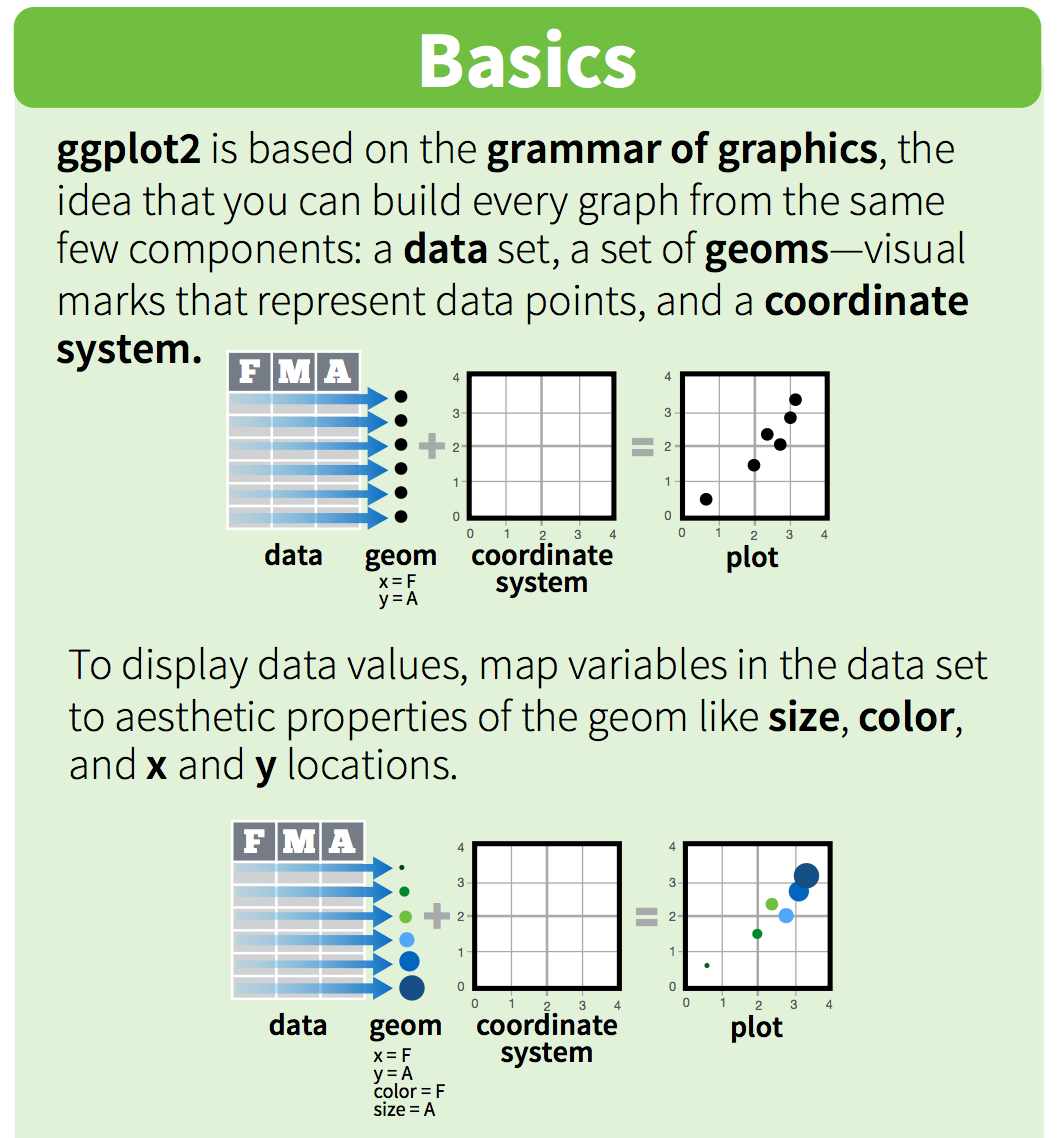
\includegraphics{img/rstudio-cheatsheet-ggplot.png}

\hypertarget{objectives-3}{%
\subsection{Objectives}\label{objectives-3}}

\begin{itemize}
\tightlist
\item
  Build several common types of graphs (scatterplot, column, line) in ggplot2
\item
  Customize gg-graph aesthetics (color, style, themes, etc.)
\item
  Update axis labels and titles
\item
  Combine compatible graph types (geoms)
\item
  Build multiseries graphs
\item
  Split up data into faceted graphs
\item
  Exporting figures with \texttt{ggsave()}
\end{itemize}

\hypertarget{resources-4}{%
\subsection{Resources}\label{resources-4}}

\begin{itemize}
\tightlist
\item
  \href{Chapter\%203\%20-\%20Data\%20Visualization\%20in\%20R\%20for\%20Data\%20Science\%20by\%20Grolemund\%20and\%20Wickham}{https://r4ds.had.co.nz/data-visualisation.html}
\item
  \href{https://www.rstudio.com/wp-content/uploads/2016/11/ggplot2-cheatsheet-2.1.pdf}{ggplot2-cheatsheet-2.1.pdf}\\
\item
  \href{http://www.cookbook-r.com/Graphs/\#graphs-with-ggplot2}{Graphs with ggplot2 - Cookbook for R}\\
\item
  \href{http://varianceexplained.org/r/why-I-use-ggplot2/}{``Why I use ggplot2'' - David Robinson Blog Post}
\end{itemize}

\hypertarget{lesson-1}{%
\section{Lesson}\label{lesson-1}}

\hypertarget{getting-started---create-a-new-.rmd-attach-packages-get-data}{%
\subsection{Getting started - Create a new .Rmd, attach packages \& get data}\label{getting-started---create-a-new-.rmd-attach-packages-get-data}}

Within your existing version-controlled R project, create a new R Markdown document with title ``Data visualization with ggplot2.'' Remove everything below the first code chunk. Knit and save the .Rmd file within your project working directory as ``my\_ggplot2''.

The \texttt{ggplot2} package is part of the \texttt{tidyverse}, so we don't need to attach it separately. Attach the \texttt{tidyverse} and \texttt{readxl} packages in the top-most code chunk of your .Rmd.

\begin{Shaded}
\begin{Highlighting}[]
\KeywordTok{library}\NormalTok{(tidyverse)}
\KeywordTok{library}\NormalTok{(readxl)}
\end{Highlighting}
\end{Shaded}

In this session, we'll use data for parks visitation from two files:

\begin{itemize}
\tightlist
\item
  A comma-separated-value (CSV) file containing visitation data for all National Parks in California (ca\_np.csv)
\item
  A single Excel worksheet containing only visitation for Channel Islands National Park
\end{itemize}

\textbf{A bit about Channel Islands National Park}: TODO

Add a new code chunk to read in the data from the \textbf{data} subfolder within your working directory.

\begin{Shaded}
\begin{Highlighting}[]
\NormalTok{ca_np <-}\StringTok{ }\KeywordTok{read_csv}\NormalTok{(}\KeywordTok{here}\NormalTok{(}\StringTok{"data"}\NormalTok{, }\StringTok{"ca_np.csv"}\NormalTok{))}
\NormalTok{ci_np <-}\StringTok{ }\KeywordTok{read_xlsx}\NormalTok{(}\KeywordTok{here}\NormalTok{(}\StringTok{"data"}\NormalTok{, }\StringTok{"ci_np.xlsx"}\NormalTok{))}
\end{Highlighting}
\end{Shaded}

Let's take a quick look at the data to see what it contains. For example:

\begin{itemize}
\tightlist
\item
  \texttt{View()}: to look at the object in spreadsheet format
\item
  \texttt{names()}: to see the variable (column) names
\item
  \texttt{summary()}: see a quick summary of each variable
\end{itemize}

\hypertarget{our-first-ggplot-graph-visitors-to-channel-islands-np}{%
\subsection{Our first ggplot graph: Visitors to Channel Islands NP}\label{our-first-ggplot-graph-visitors-to-channel-islands-np}}

To create a bare-bones ggplot graph, we need to tell R three basic things:

\begin{enumerate}
\def\labelenumi{\arabic{enumi}.}
\tightlist
\item
  We're using \texttt{ggplot}
\item
  Data we're using \& variables we're plotting (i.e., what is x and/or y?)
\item
  What type of graph we're making (the type of \emph{geom})
\end{enumerate}

Generally, that structure will look like this:

\begin{Shaded}
\begin{Highlighting}[]
\KeywordTok{ggplot}\NormalTok{(}\DataTypeTok{data =}\NormalTok{ df_name, }\KeywordTok{aes}\NormalTok{(}\DataTypeTok{x =}\NormalTok{ x_var_name, }\DataTypeTok{y =}\NormalTok{ y_var_name)) }\OperatorTok{+}
\StringTok{  }\KeywordTok{geom_type}\NormalTok{()}
\end{Highlighting}
\end{Shaded}

Breaking that down:

\begin{itemize}
\tightlist
\item
  First, tell R you're using \texttt{ggplot()}
\item
  Then, tell it the object name where variables exist (\texttt{data\ =\ df\_name})
\item
  Next, tell it the aesthetics \texttt{aes()} to specify which variables you want to plot
\item
  Then add a layer for the type of geom (graph type) with \texttt{geom\_*()} - for example, \texttt{geom\_point()} is a scatterplot, \texttt{geom\_line()} is a line graph, \texttt{geom\_col()} is a column graph, etc.
\end{itemize}

Let's do that to create a line graph of visitors to Channel Islands National Park:

\begin{Shaded}
\begin{Highlighting}[]
\KeywordTok{ggplot}\NormalTok{(}\DataTypeTok{data =}\NormalTok{ ci_np, }\KeywordTok{aes}\NormalTok{(}\DataTypeTok{x =}\NormalTok{ year, }\DataTypeTok{y =}\NormalTok{ visitors)) }\OperatorTok{+}
\StringTok{  }\KeywordTok{geom_line}\NormalTok{()}
\end{Highlighting}
\end{Shaded}

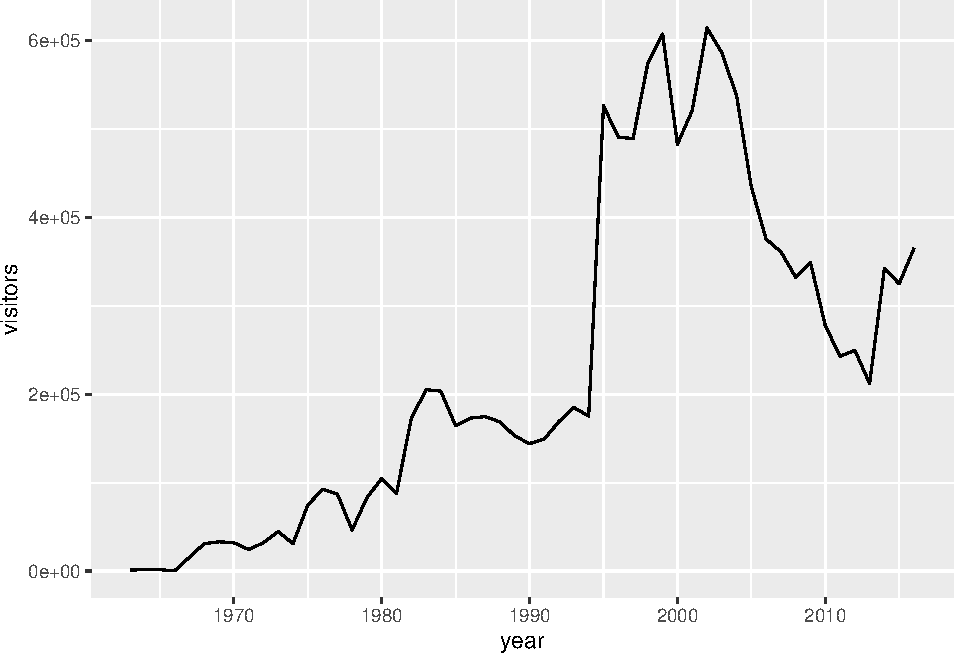
\includegraphics{R-for-Excel-Users_files/figure-latex/unnamed-chunk-59-1.pdf}

Or, we could change that to a scatterplot just by updating the \texttt{geom\_*}:

\begin{Shaded}
\begin{Highlighting}[]
\KeywordTok{ggplot}\NormalTok{(}\DataTypeTok{data =}\NormalTok{ ci_np, }\KeywordTok{aes}\NormalTok{(}\DataTypeTok{x =}\NormalTok{ year, }\DataTypeTok{y =}\NormalTok{ visitors)) }\OperatorTok{+}
\StringTok{  }\KeywordTok{geom_point}\NormalTok{()}
\end{Highlighting}
\end{Shaded}

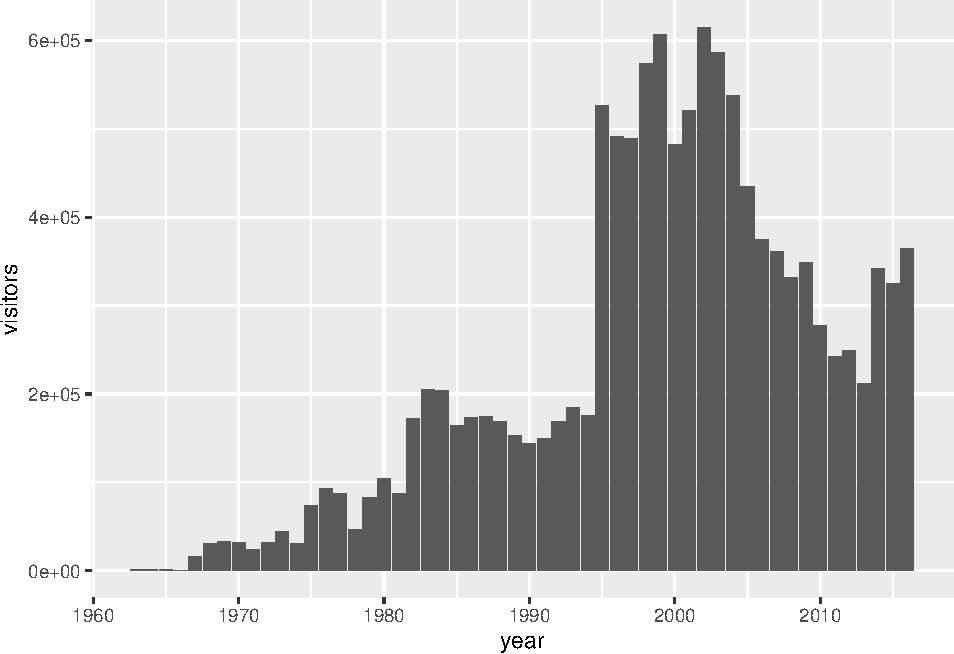
\includegraphics{R-for-Excel-Users_files/figure-latex/unnamed-chunk-60-1.pdf}

We could even do that for a column graph:

\begin{Shaded}
\begin{Highlighting}[]
\KeywordTok{ggplot}\NormalTok{(}\DataTypeTok{data =}\NormalTok{ ci_np, }\KeywordTok{aes}\NormalTok{(}\DataTypeTok{x =}\NormalTok{ year, }\DataTypeTok{y =}\NormalTok{ visitors)) }\OperatorTok{+}
\StringTok{  }\KeywordTok{geom_col}\NormalTok{()}
\end{Highlighting}
\end{Shaded}

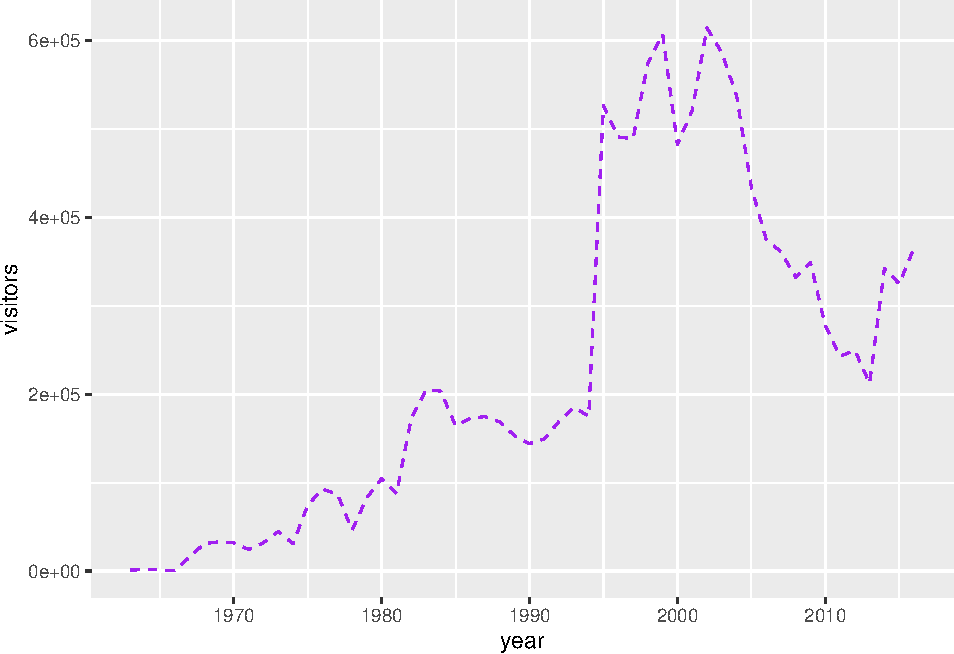
\includegraphics{R-for-Excel-Users_files/figure-latex/unnamed-chunk-61-1.pdf}

Or an area plot\ldots{}

\begin{Shaded}
\begin{Highlighting}[]
\KeywordTok{ggplot}\NormalTok{(}\DataTypeTok{data =}\NormalTok{ ci_np, }\KeywordTok{aes}\NormalTok{(}\DataTypeTok{x =}\NormalTok{ year, }\DataTypeTok{y =}\NormalTok{ visitors)) }\OperatorTok{+}
\StringTok{  }\KeywordTok{geom_area}\NormalTok{()}
\end{Highlighting}
\end{Shaded}

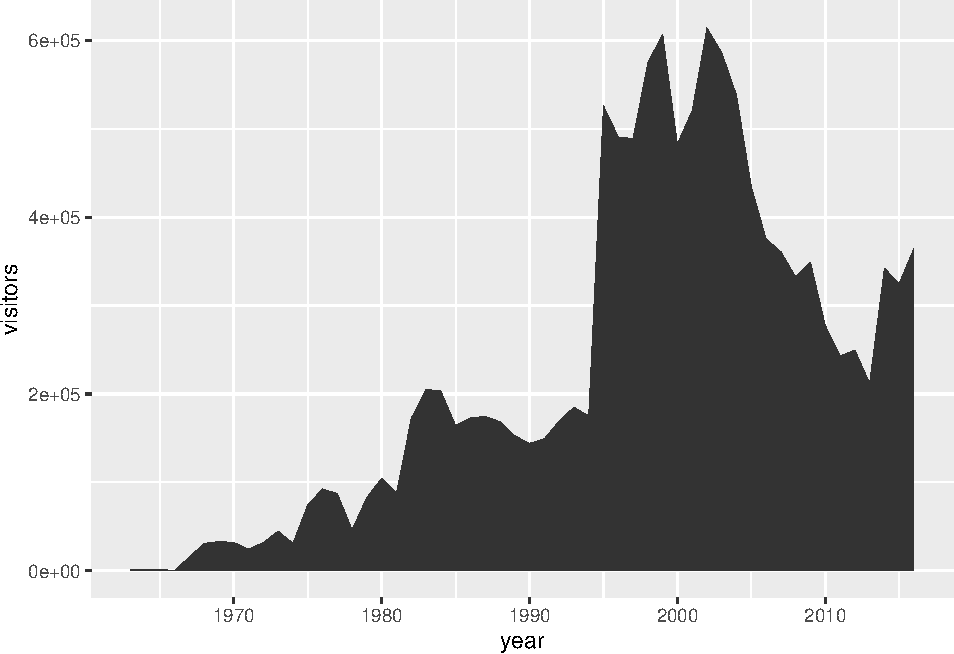
\includegraphics{R-for-Excel-Users_files/figure-latex/unnamed-chunk-62-1.pdf}

We can see that updating to different \texttt{geom\_*} types is quick, so long as the types of graphs we're switching between are compatible.

The data are there, now let's learn some customization.

\hypertarget{intro-to-customizing-ggplot-graphs}{%
\subsection{\texorpdfstring{Intro to customizing \texttt{ggplot} graphs}{Intro to customizing ggplot graphs}}\label{intro-to-customizing-ggplot-graphs}}

First, we'll customize some aesthetics (e.g.~colors, styles, axis labels, etc.) of our graphs based on non-variable values.

\begin{quote}
We can change the aesthetics of elements in a ggplot graph by adding arguments within the layer where that element is created.
\end{quote}

Some common arguments we'll use first are:

\begin{itemize}
\tightlist
\item
  \texttt{color\ =} or \texttt{colour\ =}: update point or line colors
\item
  \texttt{fill\ =}: update fill color for objects with areas
\item
  \texttt{linetype\ =}: update the line type (dashed, long dash, etc.)
\item
  \texttt{pch\ =}: update the point style
\item
  \texttt{size\ =}: update the element size (e.g.~of points or line thickness)
\item
  \texttt{alpha\ =}: update element opacity (1 = opaque, 0 = transparent)
\end{itemize}

Building on our first line graph, let's update the line color to ``purple'' and make the line type ``dashed'':

\begin{Shaded}
\begin{Highlighting}[]
\KeywordTok{ggplot}\NormalTok{(}\DataTypeTok{data =}\NormalTok{ ci_np, }\KeywordTok{aes}\NormalTok{(}\DataTypeTok{x =}\NormalTok{ year, }\DataTypeTok{y =}\NormalTok{ visitors)) }\OperatorTok{+}
\StringTok{  }\KeywordTok{geom_line}\NormalTok{(}
    \DataTypeTok{color =} \StringTok{"purple"}\NormalTok{,}
    \DataTypeTok{linetype =} \StringTok{"dashed"}
\NormalTok{  )}
\end{Highlighting}
\end{Shaded}

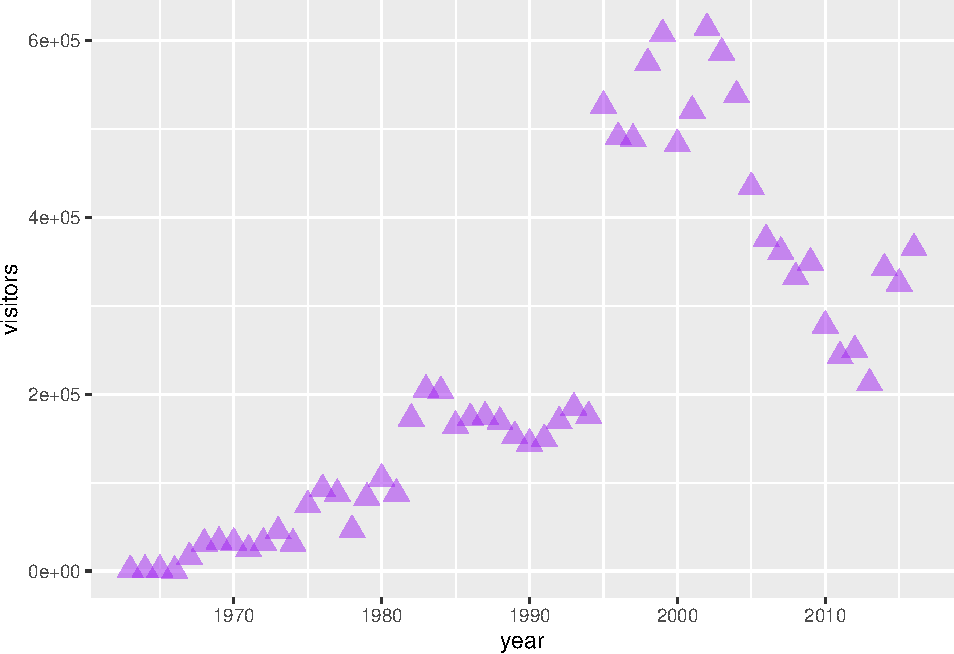
\includegraphics{R-for-Excel-Users_files/figure-latex/unnamed-chunk-63-1.pdf}

How do we know which color names ggplot will recognize? If you google ``R colors ggplot2'' you'll find a lot of good resources. Here's one: \href{http://sape.inf.usi.ch/quick-reference/ggplot2/colour}{SAPE ggplot2 colors quick reference guide}

Now let's update the point, style and size of points on our previous scatterplot graph using \texttt{color\ =}, \texttt{size\ =}, and \texttt{pch\ =} (see \texttt{?pch} for the different point styles, which can be further customized).

\begin{Shaded}
\begin{Highlighting}[]
\KeywordTok{ggplot}\NormalTok{(}\DataTypeTok{data =}\NormalTok{ ci_np, }\KeywordTok{aes}\NormalTok{(}\DataTypeTok{x =}\NormalTok{ year, }\DataTypeTok{y =}\NormalTok{ visitors)) }\OperatorTok{+}
\StringTok{  }\KeywordTok{geom_point}\NormalTok{(}\DataTypeTok{color =} \StringTok{"purple"}\NormalTok{,}
             \DataTypeTok{pch =} \DecValTok{17}\NormalTok{,}
             \DataTypeTok{size =} \DecValTok{4}\NormalTok{,}
             \DataTypeTok{alpha =} \FloatTok{0.5}\NormalTok{)}
\end{Highlighting}
\end{Shaded}

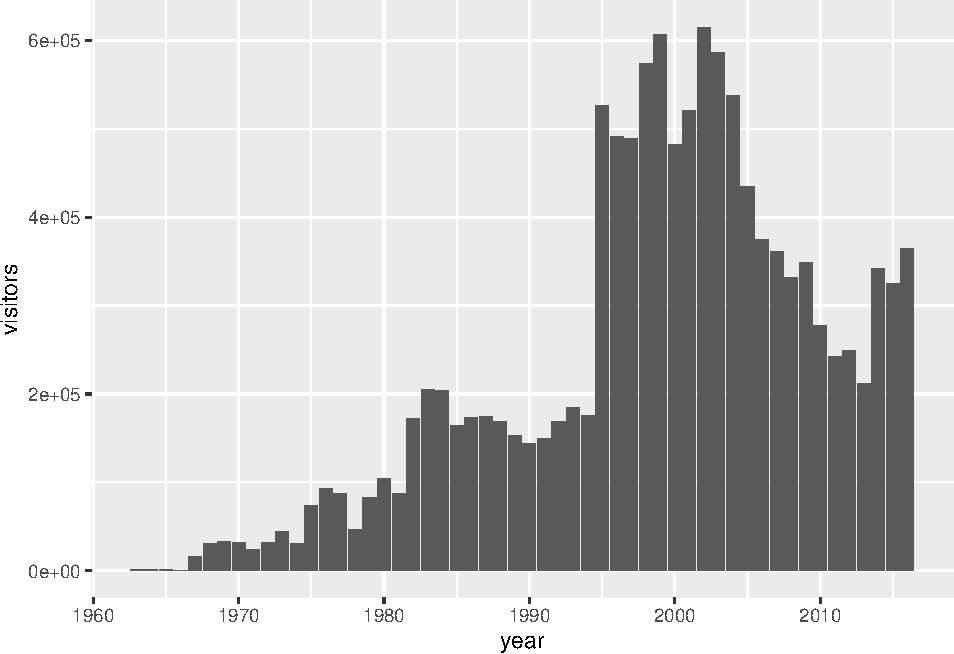
\includegraphics{R-for-Excel-Users_files/figure-latex/unnamed-chunk-64-1.pdf}

In the examples above, we have customized aesthetics based on constants that we input as arguments (e.g., the color / style / size isn't changing based on a variable characteristic or value).
Sometimes, however, we \textbf{do} want the aesthetics of a graph to depend on a variable.

\begin{quote}
When we want to customize a graph element based on a variable's characteristic or value, add the argument within \texttt{aes()} in the appropriate \texttt{geom\_*()} layer
\end{quote}

In short, if updating aesthetics based on a variable, make sure to put that argument inside of \texttt{aes()}.

\textbf{Example:} Create a ggplot scatterplot graph where the \textbf{size} and \textbf{color} of the points change based on the \textbf{number of visitors}, and make all points the same level of opacity (\texttt{alpha\ =\ 0.5}). Notice the \texttt{aes()} around the \texttt{size\ =} and \texttt{color\ =} arguments.

Also: this is overmapped and unnecessary. Avoid excessive / overcomplicated aesthetic mapping in data visualization.

\begin{Shaded}
\begin{Highlighting}[]
\KeywordTok{ggplot}\NormalTok{(}\DataTypeTok{data =}\NormalTok{ ci_np, }\KeywordTok{aes}\NormalTok{(}\DataTypeTok{x =}\NormalTok{ year, }\DataTypeTok{y =}\NormalTok{ visitors)) }\OperatorTok{+}
\StringTok{  }\KeywordTok{geom_point}\NormalTok{(}
    \KeywordTok{aes}\NormalTok{(}\DataTypeTok{size =}\NormalTok{ visitors,}
        \DataTypeTok{color =}\NormalTok{ visitors),}
    \DataTypeTok{alpha =} \FloatTok{0.5}
\NormalTok{  )}
\end{Highlighting}
\end{Shaded}

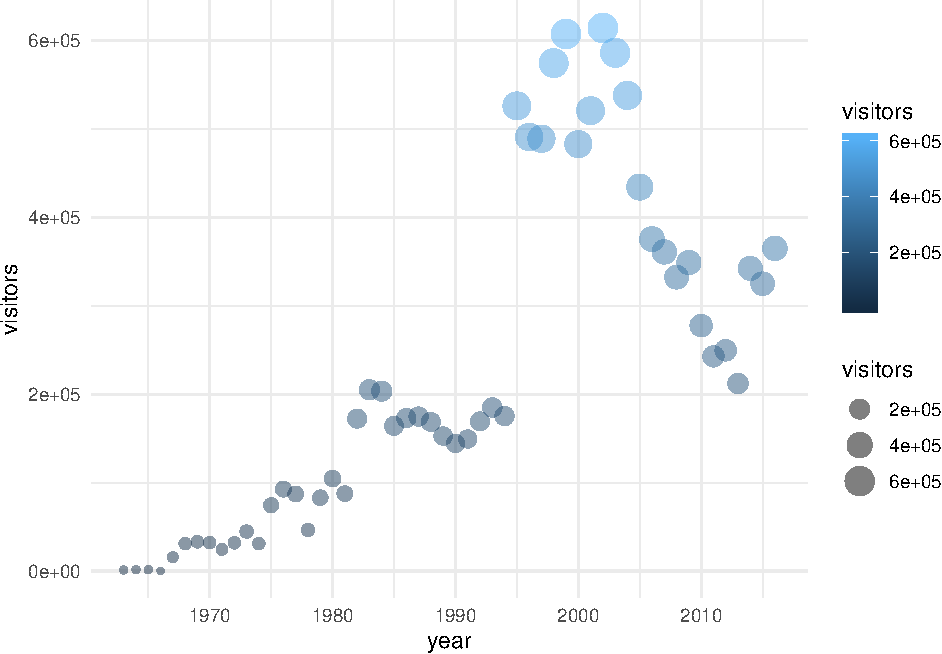
\includegraphics{R-for-Excel-Users_files/figure-latex/unnamed-chunk-65-1.pdf}

In the example above, notice that the two arguments that \textbf{do} depend on variables are within \texttt{aes()}, but since \texttt{alpha\ =\ 0.5} doesn't depend on a variable then it is \emph{outside the \texttt{aes()} but still within the \texttt{geom\_point()} layer}.

\hypertarget{ggplot2-complete-themes}{%
\subsection{ggplot2 complete themes}\label{ggplot2-complete-themes}}

While every element of a ggplot graph is manually customizable, there are also built-in themes (\texttt{theme\_*()}) that you can add to your ggplot code to make some major headway before making smaller tweaks manually.

Here are a few to try today (but also notice all the options that appear as we start typing \texttt{theme\_} into our ggplot graph code!):

\begin{itemize}
\tightlist
\item
  \texttt{theme\_light()}
\item
  \texttt{theme\_minimal()}
\item
  \texttt{theme\_bw()}
\end{itemize}

Here, let's update our previous graph with \texttt{theme\_minimal()}:

\begin{Shaded}
\begin{Highlighting}[]
\KeywordTok{ggplot}\NormalTok{(}\DataTypeTok{data =}\NormalTok{ ci_np, }\KeywordTok{aes}\NormalTok{(}\DataTypeTok{x =}\NormalTok{ year, }\DataTypeTok{y =}\NormalTok{ visitors)) }\OperatorTok{+}
\StringTok{  }\KeywordTok{geom_point}\NormalTok{(}
    \KeywordTok{aes}\NormalTok{(}\DataTypeTok{size =}\NormalTok{ visitors,}
        \DataTypeTok{color =}\NormalTok{ visitors),}
    \DataTypeTok{alpha =} \FloatTok{0.5}
\NormalTok{  ) }\OperatorTok{+}
\StringTok{  }\KeywordTok{theme_minimal}\NormalTok{()}
\end{Highlighting}
\end{Shaded}

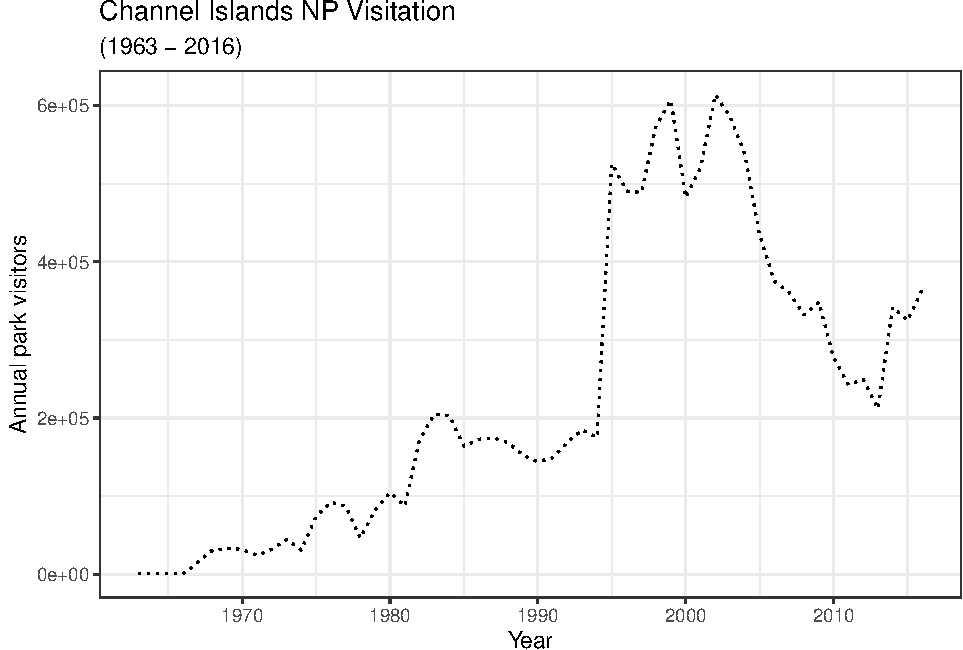
\includegraphics{R-for-Excel-Users_files/figure-latex/unnamed-chunk-66-1.pdf}

\hypertarget{updating-axis-labels-and-titles}{%
\subsection{Updating axis labels and titles}\label{updating-axis-labels-and-titles}}

Use \texttt{labs()} to update axis labels, and add a title and/or subtitle to your ggplot graph.

\begin{Shaded}
\begin{Highlighting}[]
\KeywordTok{ggplot}\NormalTok{(}\DataTypeTok{data =}\NormalTok{ ci_np, }\KeywordTok{aes}\NormalTok{(}\DataTypeTok{x =}\NormalTok{ year, }\DataTypeTok{y =}\NormalTok{ visitors)) }\OperatorTok{+}
\StringTok{  }\KeywordTok{geom_line}\NormalTok{(}\DataTypeTok{linetype =} \StringTok{"dotted"}\NormalTok{) }\OperatorTok{+}
\StringTok{  }\KeywordTok{theme_bw}\NormalTok{() }\OperatorTok{+}
\StringTok{  }\KeywordTok{labs}\NormalTok{(}
    \DataTypeTok{x =} \StringTok{"Year"}\NormalTok{,}
    \DataTypeTok{y =} \StringTok{"Annual park visitors"}\NormalTok{,}
    \DataTypeTok{title =} \StringTok{"Channel Islands NP Visitation"}\NormalTok{,}
    \DataTypeTok{subtitle =} \StringTok{"(1963 - 2016)"}
\NormalTok{  )}
\end{Highlighting}
\end{Shaded}

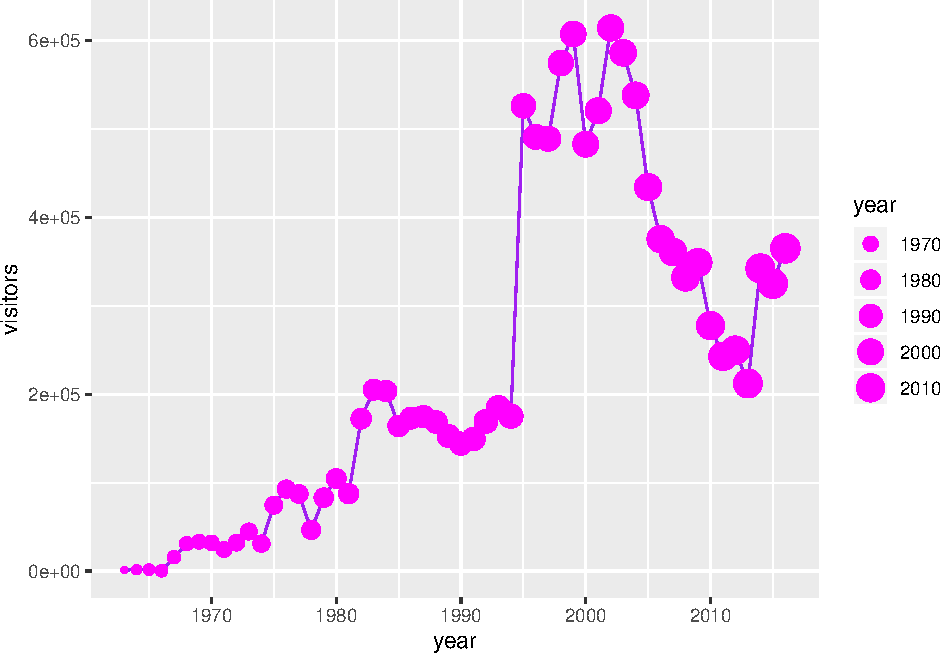
\includegraphics{R-for-Excel-Users_files/figure-latex/unnamed-chunk-67-1.pdf}

\textbf{Note}: If you want to update the formatting of axis values (for example, to convert to comma format instead of scientific format above), you can use the \texttt{scales} package options (see more from the \href{http://www.cookbook-r.com/Graphs/Axes_(ggplot2)/}{R Cookbook}).

\hypertarget{combining-compatible-geoms}{%
\subsection{Combining compatible geoms}\label{combining-compatible-geoms}}

As long as the geoms are compatible, we can layer them on top of one another to further customize a graph.

For example, adding points to a line graph:

\begin{Shaded}
\begin{Highlighting}[]
\KeywordTok{ggplot}\NormalTok{(}\DataTypeTok{data =}\NormalTok{ ci_np, }\KeywordTok{aes}\NormalTok{(}\DataTypeTok{x =}\NormalTok{ year, }\DataTypeTok{y =}\NormalTok{ visitors)) }\OperatorTok{+}
\StringTok{  }\KeywordTok{geom_line}\NormalTok{(}\DataTypeTok{color =} \StringTok{"purple"}\NormalTok{) }\OperatorTok{+}
\StringTok{  }\KeywordTok{geom_point}\NormalTok{(}\DataTypeTok{color =} \StringTok{"magenta"}\NormalTok{,}
             \KeywordTok{aes}\NormalTok{(}\DataTypeTok{size =}\NormalTok{ year))}
\end{Highlighting}
\end{Shaded}

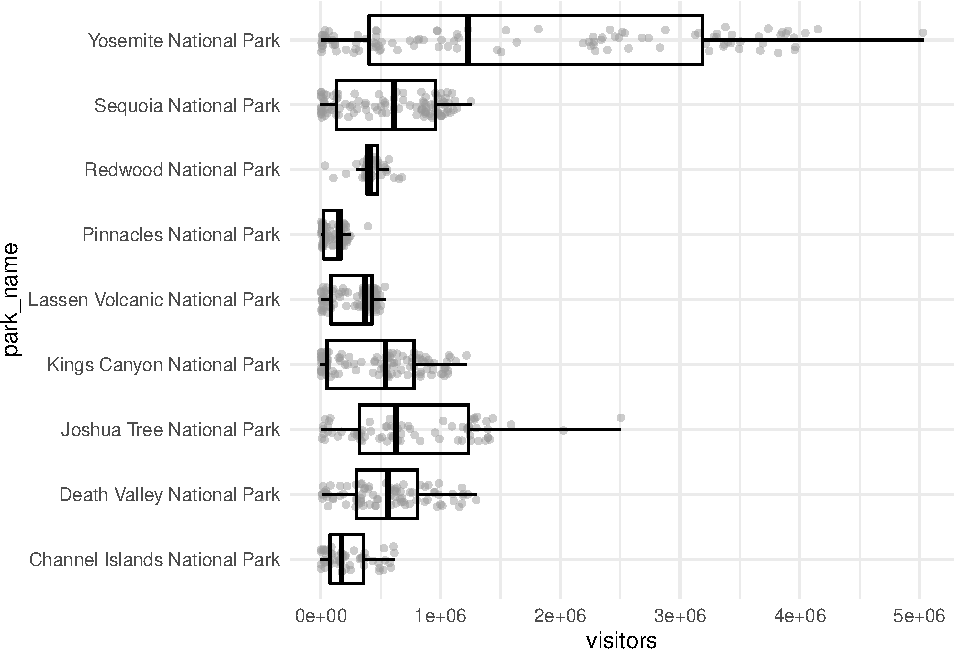
\includegraphics{R-for-Excel-Users_files/figure-latex/unnamed-chunk-68-1.pdf}

Or, combine a column and line graph (not sure why you'd want to do this, but you can):

\begin{Shaded}
\begin{Highlighting}[]
\KeywordTok{ggplot}\NormalTok{(}\DataTypeTok{data =}\NormalTok{ ci_np, }\KeywordTok{aes}\NormalTok{(}\DataTypeTok{x =}\NormalTok{ year, }\DataTypeTok{y =}\NormalTok{ visitors)) }\OperatorTok{+}
\StringTok{  }\KeywordTok{geom_col}\NormalTok{(}\DataTypeTok{fill =} \StringTok{"orange"}\NormalTok{,}
           \DataTypeTok{color =} \StringTok{"purple"}\NormalTok{) }\OperatorTok{+}
\StringTok{  }\KeywordTok{geom_line}\NormalTok{()}
\end{Highlighting}
\end{Shaded}

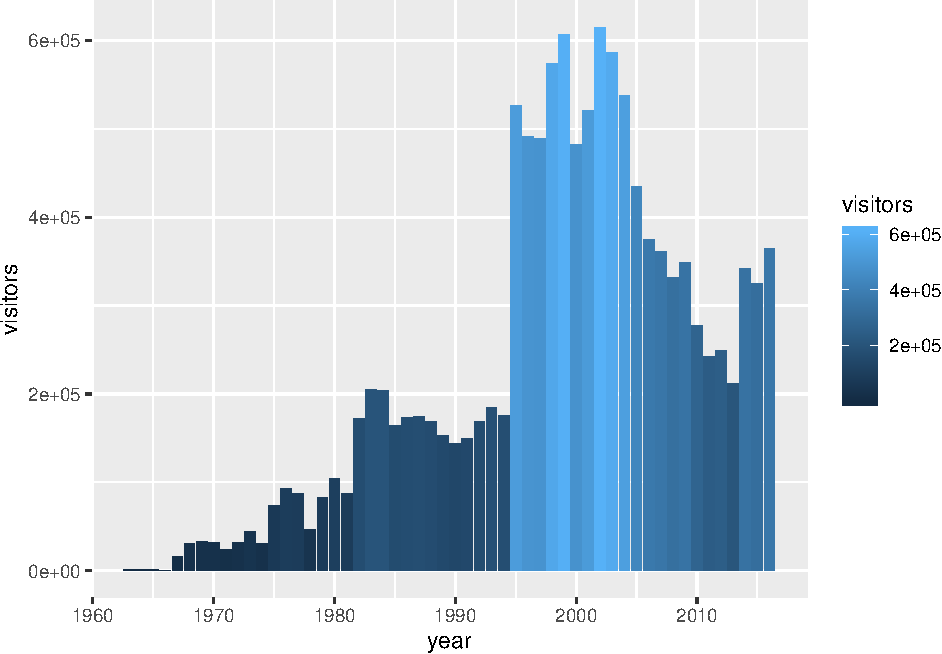
\includegraphics{R-for-Excel-Users_files/figure-latex/unnamed-chunk-69-1.pdf}

\hypertarget{multi-series-ggplot-graphs}{%
\subsection{Multi-series ggplot graphs}\label{multi-series-ggplot-graphs}}

In the examples above, we only had a single series - visitation at Channel Islands National Park. Often we'll want to visualize multiple series. For example, from the \texttt{ca\_np} object we have stored, we might want to plot visitation for \emph{all} California National Parks.

To do that, we need to add an aesthetic that lets \texttt{ggplot} know how things are going to be grouped. A demonstration of why that's important - what happens if we \emph{don't} let ggplot know how to group things?

\begin{Shaded}
\begin{Highlighting}[]
\KeywordTok{ggplot}\NormalTok{(}\DataTypeTok{data =}\NormalTok{ ca_np, }\KeywordTok{aes}\NormalTok{(}\DataTypeTok{x =}\NormalTok{ year, }\DataTypeTok{y =}\NormalTok{ visitors)) }\OperatorTok{+}
\StringTok{  }\KeywordTok{geom_line}\NormalTok{()}
\end{Highlighting}
\end{Shaded}

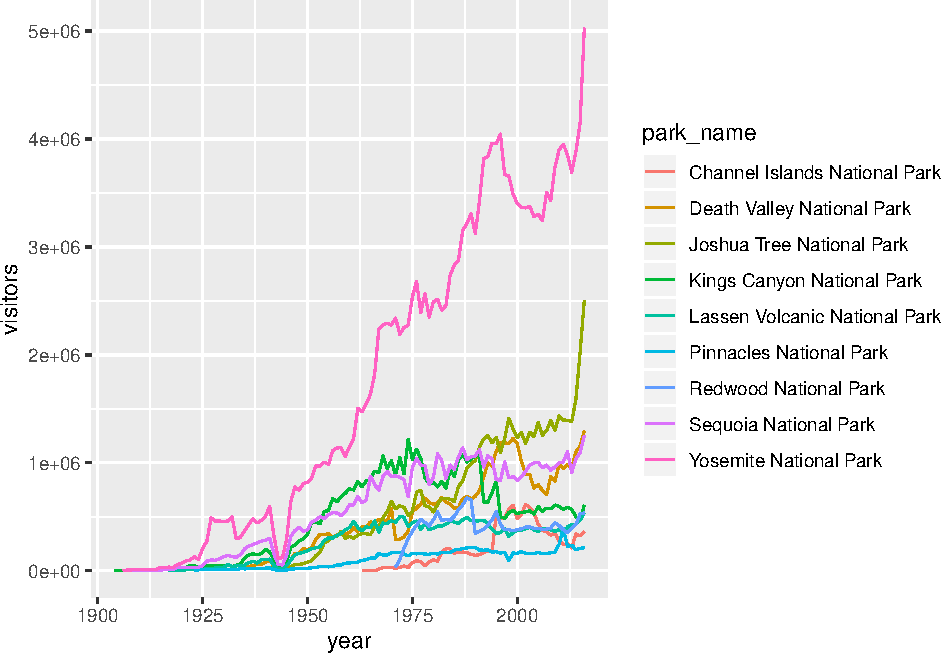
\includegraphics{R-for-Excel-Users_files/figure-latex/unnamed-chunk-70-1.pdf}

Well that's definitely a mess, and it's because ggplot has no idea that these \textbf{should be different series based on the different parks that appear in the `park\_name' column}.

We can make sure R does know by updating an aesthetic based on \emph{park\_name}:

\begin{Shaded}
\begin{Highlighting}[]
\KeywordTok{ggplot}\NormalTok{(}\DataTypeTok{data =}\NormalTok{ ca_np, }\KeywordTok{aes}\NormalTok{(}\DataTypeTok{x =}\NormalTok{ year, }\DataTypeTok{y =}\NormalTok{ visitors, }\DataTypeTok{color =}\NormalTok{ park_name)) }\OperatorTok{+}
\StringTok{  }\KeywordTok{geom_line}\NormalTok{()}
\end{Highlighting}
\end{Shaded}

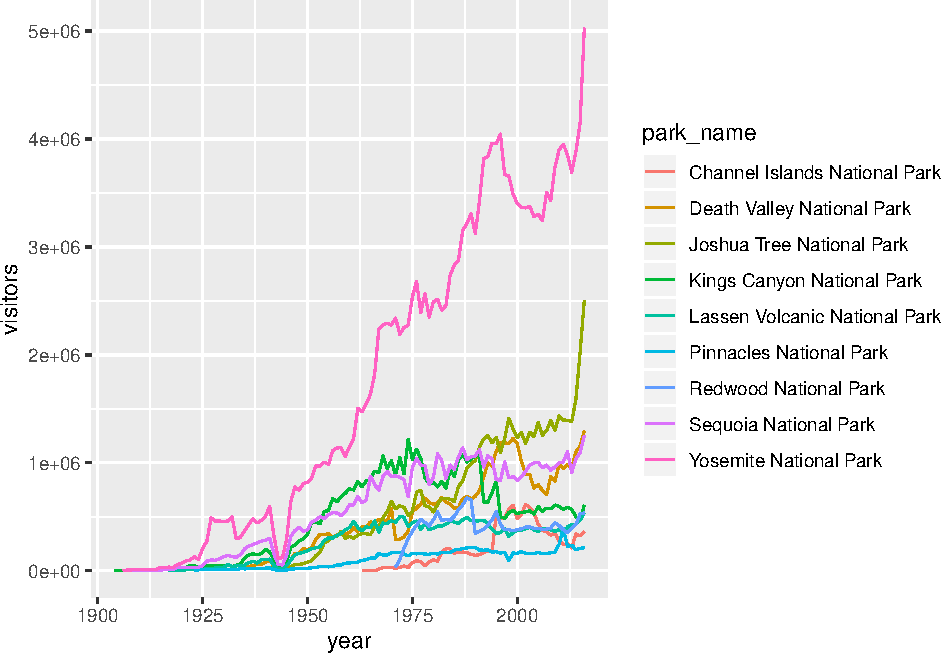
\includegraphics{R-for-Excel-Users_files/figure-latex/unnamed-chunk-71-1.pdf}

\textbf{Note}: You could also add that aesthetic (\texttt{color\ =\ park\_name}) in the \texttt{geom\_line()} layer, instead of in the topmost \texttt{ggplot()} layer.

\hypertarget{faceting-ggplot-graphs}{%
\subsection{Faceting ggplot graphs}\label{faceting-ggplot-graphs}}

When we facet graphs, we split them up into multiple plotting panels, where each panel contains a subset of the data. In our case, we'll split the graph above into different panels, each containing visitation data for a single park.

Also notice that any general theme changes made will be applied to \emph{all} of the graphs.

\begin{Shaded}
\begin{Highlighting}[]
\KeywordTok{ggplot}\NormalTok{(}\DataTypeTok{data =}\NormalTok{ ca_np, }\KeywordTok{aes}\NormalTok{(}\DataTypeTok{x =}\NormalTok{ year, }\DataTypeTok{y =}\NormalTok{ visitors, }\DataTypeTok{color =}\NormalTok{ park_name)) }\OperatorTok{+}
\StringTok{  }\KeywordTok{geom_line}\NormalTok{(}\DataTypeTok{show.legend =} \OtherTok{FALSE}\NormalTok{) }\OperatorTok{+}
\StringTok{  }\KeywordTok{theme_light}\NormalTok{() }\OperatorTok{+}\StringTok{ }
\StringTok{  }\KeywordTok{labs}\NormalTok{(}\DataTypeTok{x =} \StringTok{"year"}\NormalTok{, }\DataTypeTok{y =} \StringTok{"annual visitors"}\NormalTok{) }\OperatorTok{+}
\StringTok{  }\KeywordTok{facet_wrap}\NormalTok{(}\OperatorTok{~}\StringTok{ }\NormalTok{park_name)}
\end{Highlighting}
\end{Shaded}

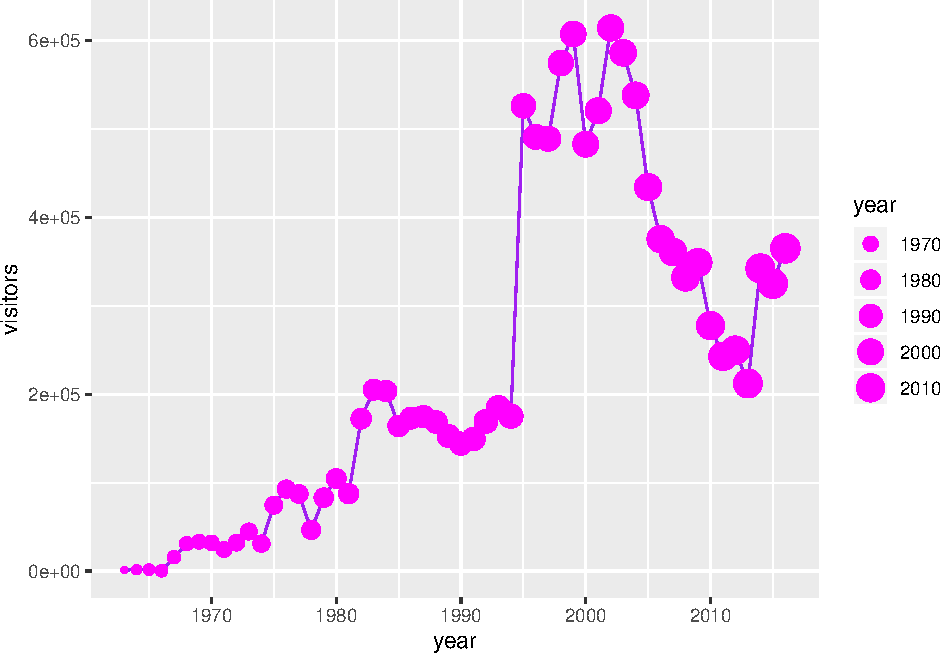
\includegraphics{R-for-Excel-Users_files/figure-latex/unnamed-chunk-72-1.pdf}

\hypertarget{exporting-a-ggplot-graph-with-ggsave}{%
\subsection{\texorpdfstring{Exporting a ggplot graph with \texttt{ggsave()}}{Exporting a ggplot graph with ggsave()}}\label{exporting-a-ggplot-graph-with-ggsave}}

If we want our graph to appear in a knitted html, then we don't need to do anything else. But often we'll need a saved image file, of specific size and resolution, to share or for publication.

\texttt{ggsave()} will export the \emph{most recently run} ggplot graph by default (\texttt{plot\ =\ last\_plot()}), unless you give it the name of a different saved ggplot object. Some common arguments for \texttt{ggsave()}:

\begin{itemize}
\tightlist
\item
  \texttt{width\ =}: set exported image width (default inches)
\item
  \texttt{height\ =}: set exported image height (default height)
\item
  \texttt{dpi\ =}: set dpi (dots per inch)
\end{itemize}

So to export the faceted graph above at 180 dpi, width a width of 8" and a height of 7", we can use:

\begin{Shaded}
\begin{Highlighting}[]
\KeywordTok{ggsave}\NormalTok{(}\KeywordTok{here}\NormalTok{(}\StringTok{"figures"}\NormalTok{, }\StringTok{"np_graph.jpg"}\NormalTok{), }\DataTypeTok{dpi =} \DecValTok{180}\NormalTok{, }\DataTypeTok{width =} \DecValTok{8}\NormalTok{, }\DataTypeTok{height =} \DecValTok{7}\NormalTok{)}
\end{Highlighting}
\end{Shaded}

Notice that a .jpg image of that name and size is now stored in your project working directory. You can change the type of exported image, too (e.g.~pdf, tiff, eps, png, mmp, svg).

\hypertarget{one-final-graph-example-jitter-and-boxplots}{%
\subsection{One final graph example: jitter and boxplots}\label{one-final-graph-example-jitter-and-boxplots}}

For the record: this is not a good option for showing the visitation data because values are not independent observations of a random variable. But, for the purposes of showing a graph, we'll use visitation as our continuous measured variable in a jitter + boxplot anyway.

\begin{Shaded}
\begin{Highlighting}[]
\KeywordTok{ggplot}\NormalTok{(}\DataTypeTok{data =}\NormalTok{ ca_np, }\KeywordTok{aes}\NormalTok{(}\DataTypeTok{x =}\NormalTok{ park_name, }\DataTypeTok{y =}\NormalTok{ visitors)) }\OperatorTok{+}
\StringTok{  }\KeywordTok{geom_jitter}\NormalTok{(}\DataTypeTok{alpha =} \FloatTok{0.5}\NormalTok{,}
              \DataTypeTok{color =} \StringTok{"gray60"}\NormalTok{,}
              \DataTypeTok{width =} \FloatTok{0.2}\NormalTok{,}
              \DataTypeTok{size =} \DecValTok{1}\NormalTok{) }\OperatorTok{+}
\StringTok{  }\KeywordTok{geom_boxplot}\NormalTok{(}\DataTypeTok{fill =} \OtherTok{NA}\NormalTok{,}
               \DataTypeTok{color =} \StringTok{"black"}\NormalTok{,}
               \DataTypeTok{outlier.color =} \OtherTok{NA}\NormalTok{) }\OperatorTok{+}
\StringTok{  }\KeywordTok{coord_flip}\NormalTok{() }\OperatorTok{+}
\StringTok{  }\KeywordTok{theme_minimal}\NormalTok{()}
\end{Highlighting}
\end{Shaded}

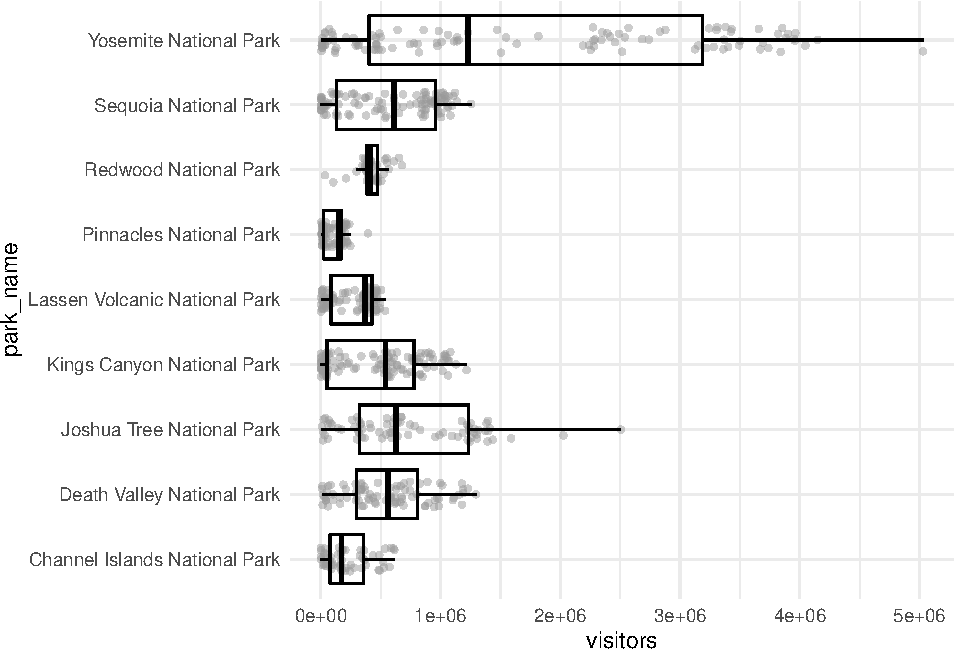
\includegraphics{R-for-Excel-Users_files/figure-latex/unnamed-chunk-75-1.pdf}

\hypertarget{efficiency-tips-3}{%
\section{Efficiency Tips}\label{efficiency-tips-3}}

\hypertarget{pivot}{%
\chapter{\texorpdfstring{\texttt{dplyr} and Pivot Tables}{dplyr and Pivot Tables}}\label{pivot}}

\hypertarget{summary-4}{%
\section{Summary}\label{summary-4}}

Pivot tables are powerful tools in Excel for summarizing data in different ways. We will create these tables using the \texttt{group\_by} and \texttt{summarize} functions from the \texttt{dplyr} package (part of the Tidyverse). We will also learn how to format tables and practice creating a reproducible report using RMarkdown and sharing it with GitHub.

\hypertarget{objectives-4}{%
\section{Objectives}\label{objectives-4}}

In R, we can use dplyr for pivot tables by using 2 main verbs in combination: \texttt{group\_by} and \texttt{summarize}. We will also continue to emphasize reproducibility in all our analyses.

\begin{itemize}
\tightlist
\item
  Discuss pivot tables in Excel
\item
  Introduce \texttt{group\_by()\ \%\textgreater{}\%\ summarize()} from the \texttt{dplyr} package
\item
  Format tables with the \texttt{DT} and \texttt{knitr} packages
\item
  Practice our reproducible workflow with RMarkdown and GitHub
\end{itemize}

\hypertarget{resources-5}{%
\section{Resources}\label{resources-5}}

\begin{itemize}
\tightlist
\item
  \href{https://dplyr.tidyverse.org/}{dplyr.tidyverse.org}
\item
  \href{https://r4ds.had.co.nz/transform.html}{R for Data Science: Transform Chapter}
\item
  \href{https://youtu.be/g530cnFfk8Y}{Intro to Pivot Tables I-III} by Excel Campus (YouTube)
\end{itemize}

\hypertarget{pivot-table-overview}{%
\section{Pivot table overview}\label{pivot-table-overview}}

\href{https://en.wikipedia.org/wiki/Pivot_table}{Wikipedia describes a pivot table} as a ``table of statistics that summarizes the data of a more extensive table\ldots{}This summary might include sums, averages, or other statistics, which the pivot table groups together in a meaningful way.'' Fun fact: it also says that ``Although pivot table is a generic term, Microsoft trademarked PivotTable in the United States in 1994.''

Pivot tables are a really powerful tool for summarizing data, and we can have similar functionality in R --- as well as nicely automating and reporting these tables. We will learn about this using data about lobsters and will go back and forth between R and Excel as we learn.

Let's start off in R, and have a look at the data.

\hypertarget{rmarkdown-setup}{%
\section{RMarkdown setup}\label{rmarkdown-setup}}

Let's start a new RMarkdown file in our repo, at the top-level (where it will be created by default in our Project). I'll call mine \texttt{pivot\_lobsters.Rmd}.

In the setup chunk, let's attach our libraries and read in our lobster data. In addition to the \texttt{tidyverse} package we will also use the \texttt{skimr} package. You will have to install it, but don't want it to be installed every time you write your code. The following is a nice convention for having the install instructions available (on the same line) as the \texttt{library()} call.

\begin{Shaded}
\begin{Highlighting}[]
\CommentTok{## attach libraries}
\KeywordTok{library}\NormalTok{(tidyverse)}
\KeywordTok{library}\NormalTok{(readxl)}
\KeywordTok{library}\NormalTok{(here)}
\KeywordTok{library}\NormalTok{(skimr) }\CommentTok{# install.packages('skimr')}

\CommentTok{## read in data}
\NormalTok{lobsters <-}\StringTok{ }\KeywordTok{read_xlsx}\NormalTok{(}\KeywordTok{here}\NormalTok{(}\StringTok{"data/lobsters_curated.xlsx"}\NormalTok{))}
\end{Highlighting}
\end{Shaded}

Let's add a code chunk and explore the data in a few ways.

\begin{Shaded}
\begin{Highlighting}[]
\CommentTok{# explore data}
\KeywordTok{head}\NormalTok{(lobsters) }\CommentTok{# year and month as well as a column for date}
\end{Highlighting}
\end{Shaded}

\begin{verbatim}
## # A tibble: 6 x 7
##    year month date    site  transect replicate size_mm
##   <dbl> <dbl> <chr>   <chr>    <dbl> <chr>       <dbl>
## 1  2012     8 8/20/12 ivee         3 A              70
## 2  2012     8 8/20/12 ivee         3 B              60
## 3  2012     8 8/20/12 ivee         3 B              65
## 4  2012     8 8/20/12 ivee         3 B              70
## 5  2012     8 8/20/12 ivee         3 B              85
## 6  2012     8 8/20/12 ivee         3 C              60
\end{verbatim}

\texttt{head()} gives us a look at the first rows of the data (6 by default). I like this because I can see the column names and get a sense of the shape of the data. I can also see the class of each column (double or character)

In this data set, every row is a unique observation. This is called ``uncounted'' data; you'll see there is no row for how many lobsters were seen because each row is an observation, or an ``n of 1''.

\begin{Shaded}
\begin{Highlighting}[]
\CommentTok{# explore data}
\KeywordTok{summary}\NormalTok{(lobsters) }
\end{Highlighting}
\end{Shaded}

\begin{verbatim}
##       year          month           date               site          
##  Min.   :2012   Min.   :8.000   Length:2893        Length:2893       
##  1st Qu.:2014   1st Qu.:8.000   Class :character   Class :character  
##  Median :2015   Median :8.000   Mode  :character   Mode  :character  
##  Mean   :2015   Mean   :8.037                                        
##  3rd Qu.:2016   3rd Qu.:8.000                                        
##  Max.   :2016   Max.   :9.000                                        
##                                                                      
##     transect      replicate            size_mm      
##  Min.   :1.000   Length:2893        Min.   : 18.00  
##  1st Qu.:2.000   Class :character   1st Qu.: 62.00  
##  Median :3.000   Mode  :character   Median : 72.00  
##  Mean   :3.723                      Mean   : 71.38  
##  3rd Qu.:5.000                      3rd Qu.: 81.00  
##  Max.   :9.000                      Max.   :165.00  
##                                     NA's   :5
\end{verbatim}

\texttt{summary} gives us summary statistics for each variable (column). I like this for numeric columns, but it doesn't give a lot of useful information for non-numeric data. To have a look there I like using the skimr package:

\begin{Shaded}
\begin{Highlighting}[]
\CommentTok{# explore data}
\NormalTok{skimr}\OperatorTok{::}\KeywordTok{skim}\NormalTok{(lobsters) }
\end{Highlighting}
\end{Shaded}

\label{tab:skim-lobsters}Data summary

Name

lobsters

Number of rows

2893

Number of columns

7

\_\_\_\_\_\_\_\_\_\_\_\_\_\_\_\_\_\_\_\_\_\_\_

Column type frequency:

character

3

numeric

4

\_\_\_\_\_\_\_\_\_\_\_\_\_\_\_\_\_\_\_\_\_\_\_\_

Group variables

None

\textbf{Variable type: character}

skim\_variable

n\_missing

complete\_rate

min

max

empty

n\_unique

whitespace

date

0

1

6

7

0

28

0

site

0

1

4

4

0

5

0

replicate

0

1

1

1

0

4

0

\textbf{Variable type: numeric}

skim\_variable

n\_missing

complete\_rate

mean

sd

p0

p25

p50

p75

p100

hist

year

0

1

2014.70

1.19

2012

2014

2015

2016

2016

▂▂▃▇▆

month

0

1

8.04

0.19

8

8

8

8

9

▇▁▁▁▁

transect

0

1

3.72

2.30

1

2

3

5

9

▇▅▃▂▂

size\_mm

5

1

71.38

14.75

18

62

72

81

165

▁▇▆▁▁

This \texttt{skimr::} notation is a reminder to me that \texttt{skim} is from the \texttt{skimr} package. It is a nice convention: it's a reminder to others (especially you!).

\texttt{skim} lets us look more at each variable. I particularly like looking at missing data. There are 6 missing values in the \texttt{size\_mm} variable.

We can also make a quick plot to have a look at these data, and use our new ggplot2 skills. Let's make a bar chart by year for each site

\begin{Shaded}
\begin{Highlighting}[]
\KeywordTok{ggplot}\NormalTok{(lobsters, }\KeywordTok{aes}\NormalTok{(}\DataTypeTok{x =}\NormalTok{ year)) }\OperatorTok{+}
\StringTok{  }\KeywordTok{geom_bar}\NormalTok{() }\OperatorTok{+}
\StringTok{  }\KeywordTok{facet_wrap}\NormalTok{(}\OperatorTok{~}\NormalTok{site)}
\end{Highlighting}
\end{Shaded}

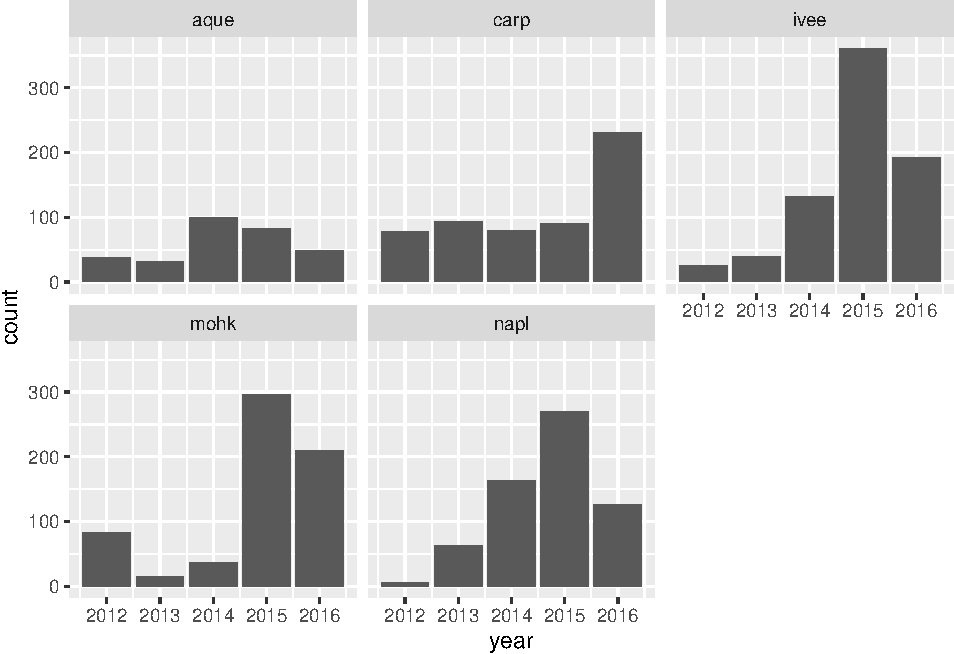
\includegraphics{R-for-Excel-Users_files/figure-latex/plot-lobsters-1.pdf}

(geom\_bar() counts things and geom\_col() is for values within the data (mean))

\hypertarget{our-task}{%
\subsection{Our task}\label{our-task}}

So this is all great to get a quick look. But what if we needed to report to someone about how the average size of lobsters has changed over time across sites?

To answer this we need to do a pivot table in Excel, or data wrangling in R.

Let's start by having a quick look at what pivot tables can do in Excel.

\hypertarget{pivot-table-demo}{%
\section{Pivot table demo}\label{pivot-table-demo}}

Let's make a pivot table with our lobster data.

Let's start off with how many lobsters were counted each year. I want a count of rows by year So to do this in Excel we would initiate the Pivot Table Process:

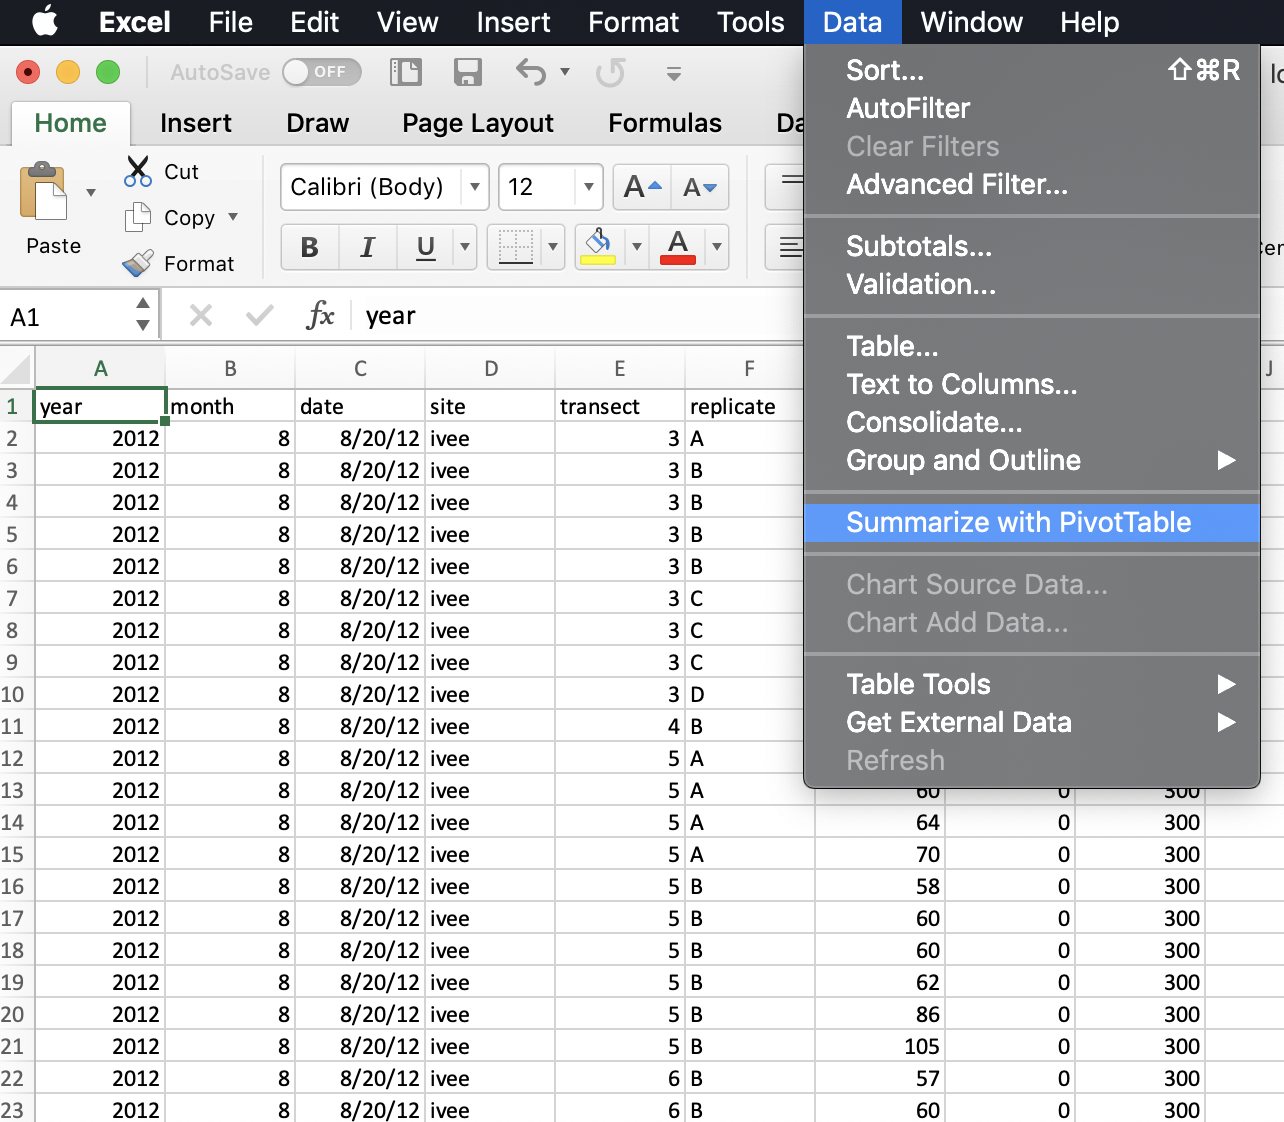
\includegraphics[width=0.6\linewidth]{img/pivot-table-menu}

And it will do its best to find the data I would like to include in my Pivot Table (it can have difficulty with non-rectangular or ``non-tidy'' data), and suggest we make this in a new sheet:

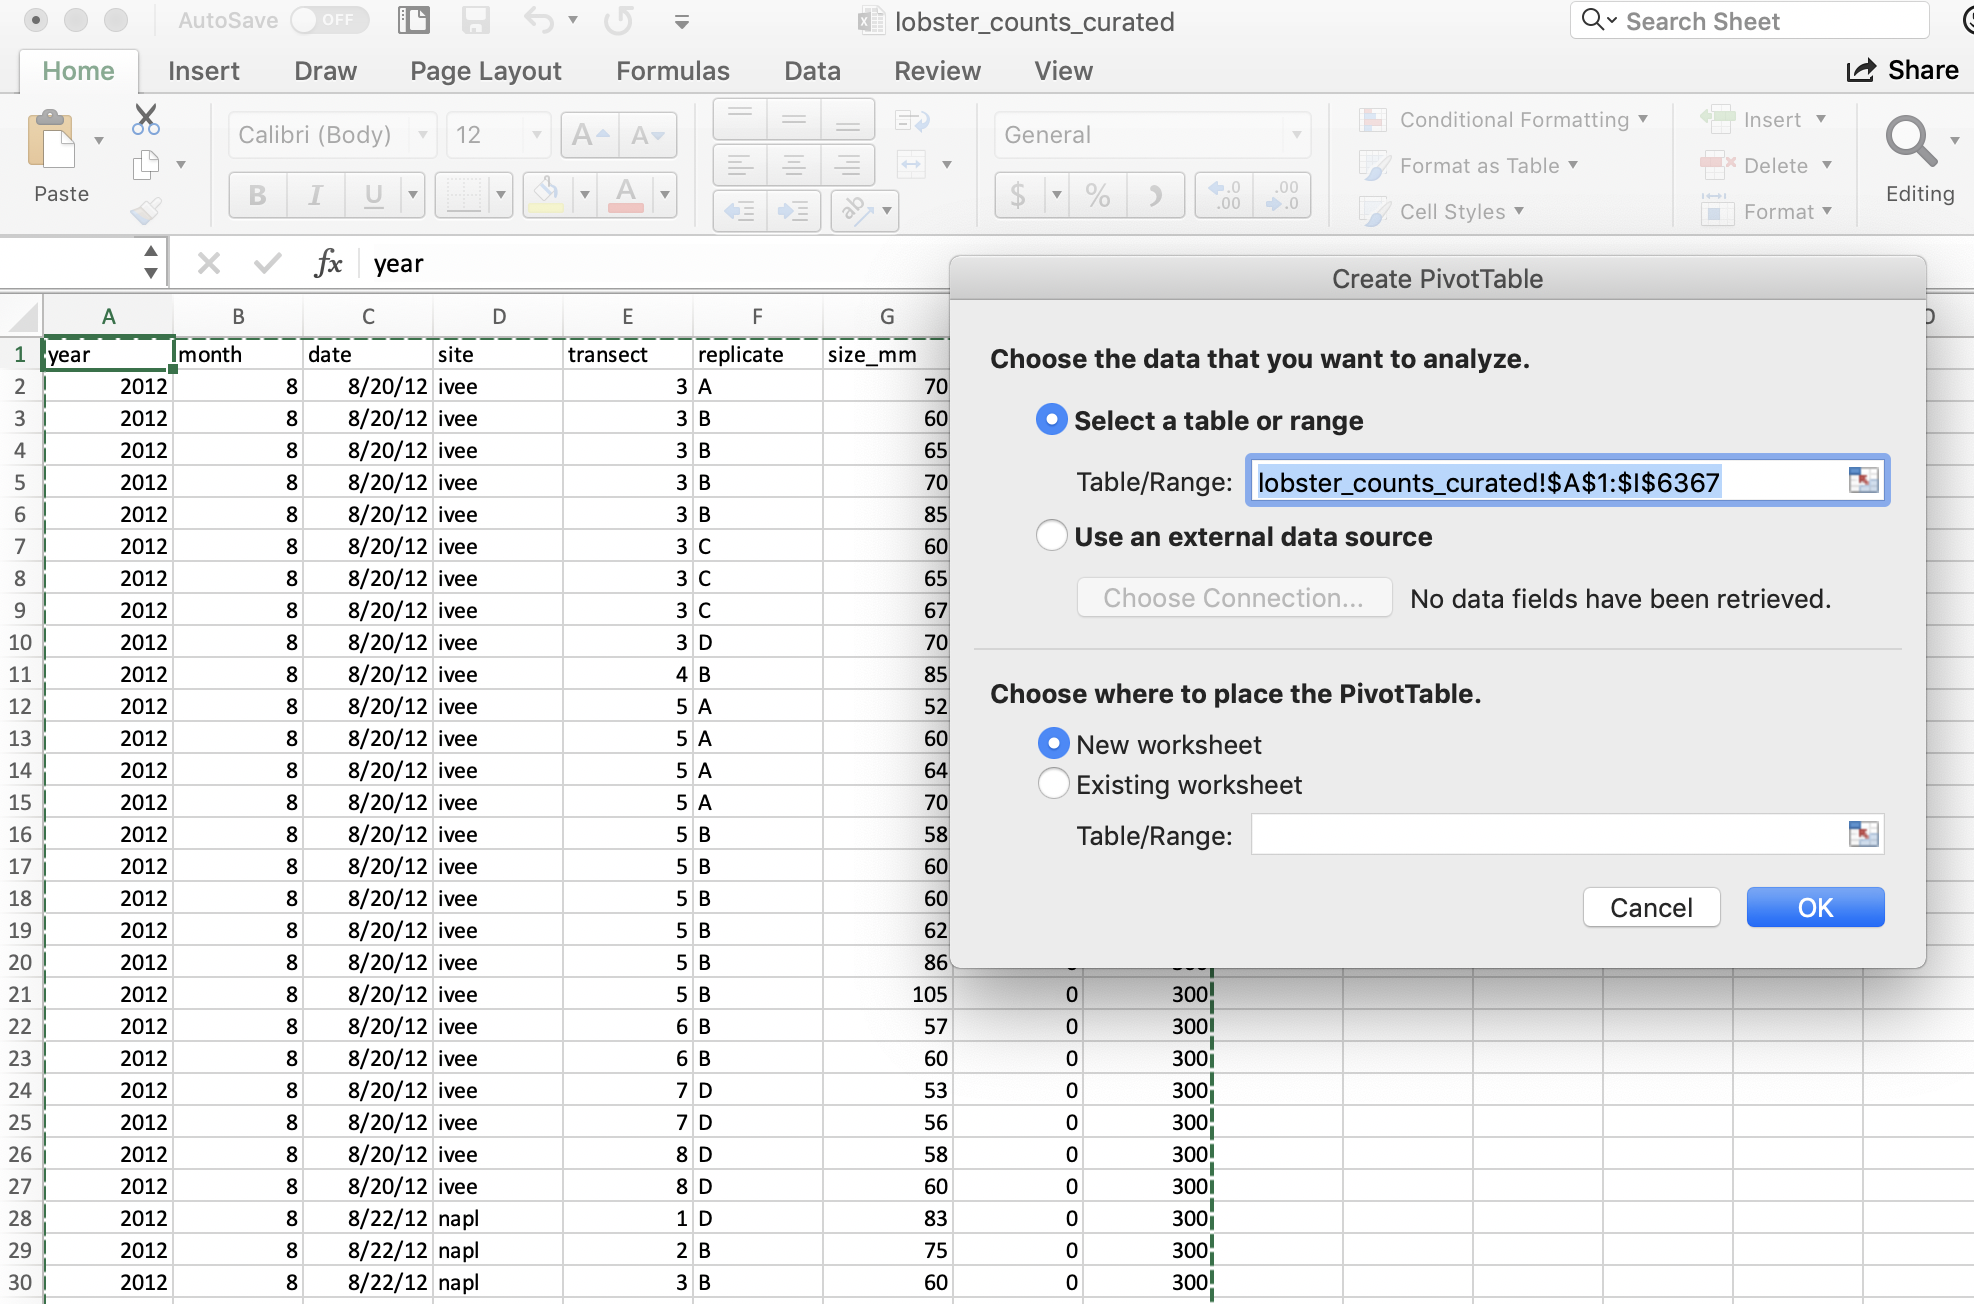
\includegraphics[width=0.6\linewidth]{img/pivot-table-create}

And then we'll get a little wizard to help us create the Pivot Table.

\hypertarget{pivot-one-variable}{%
\subsection{pivot one variable}\label{pivot-one-variable}}

I want to summarize by year, so I drag ``year'' down into the ``Rows'' box, and to get the counts by year I actually drag the same variable, ``year'' into the ``Values'' box. And it will create a Pivot Table for me! But ``sum'' as the default summary statistic, so I can click the little ``I'' icon to change this to count.

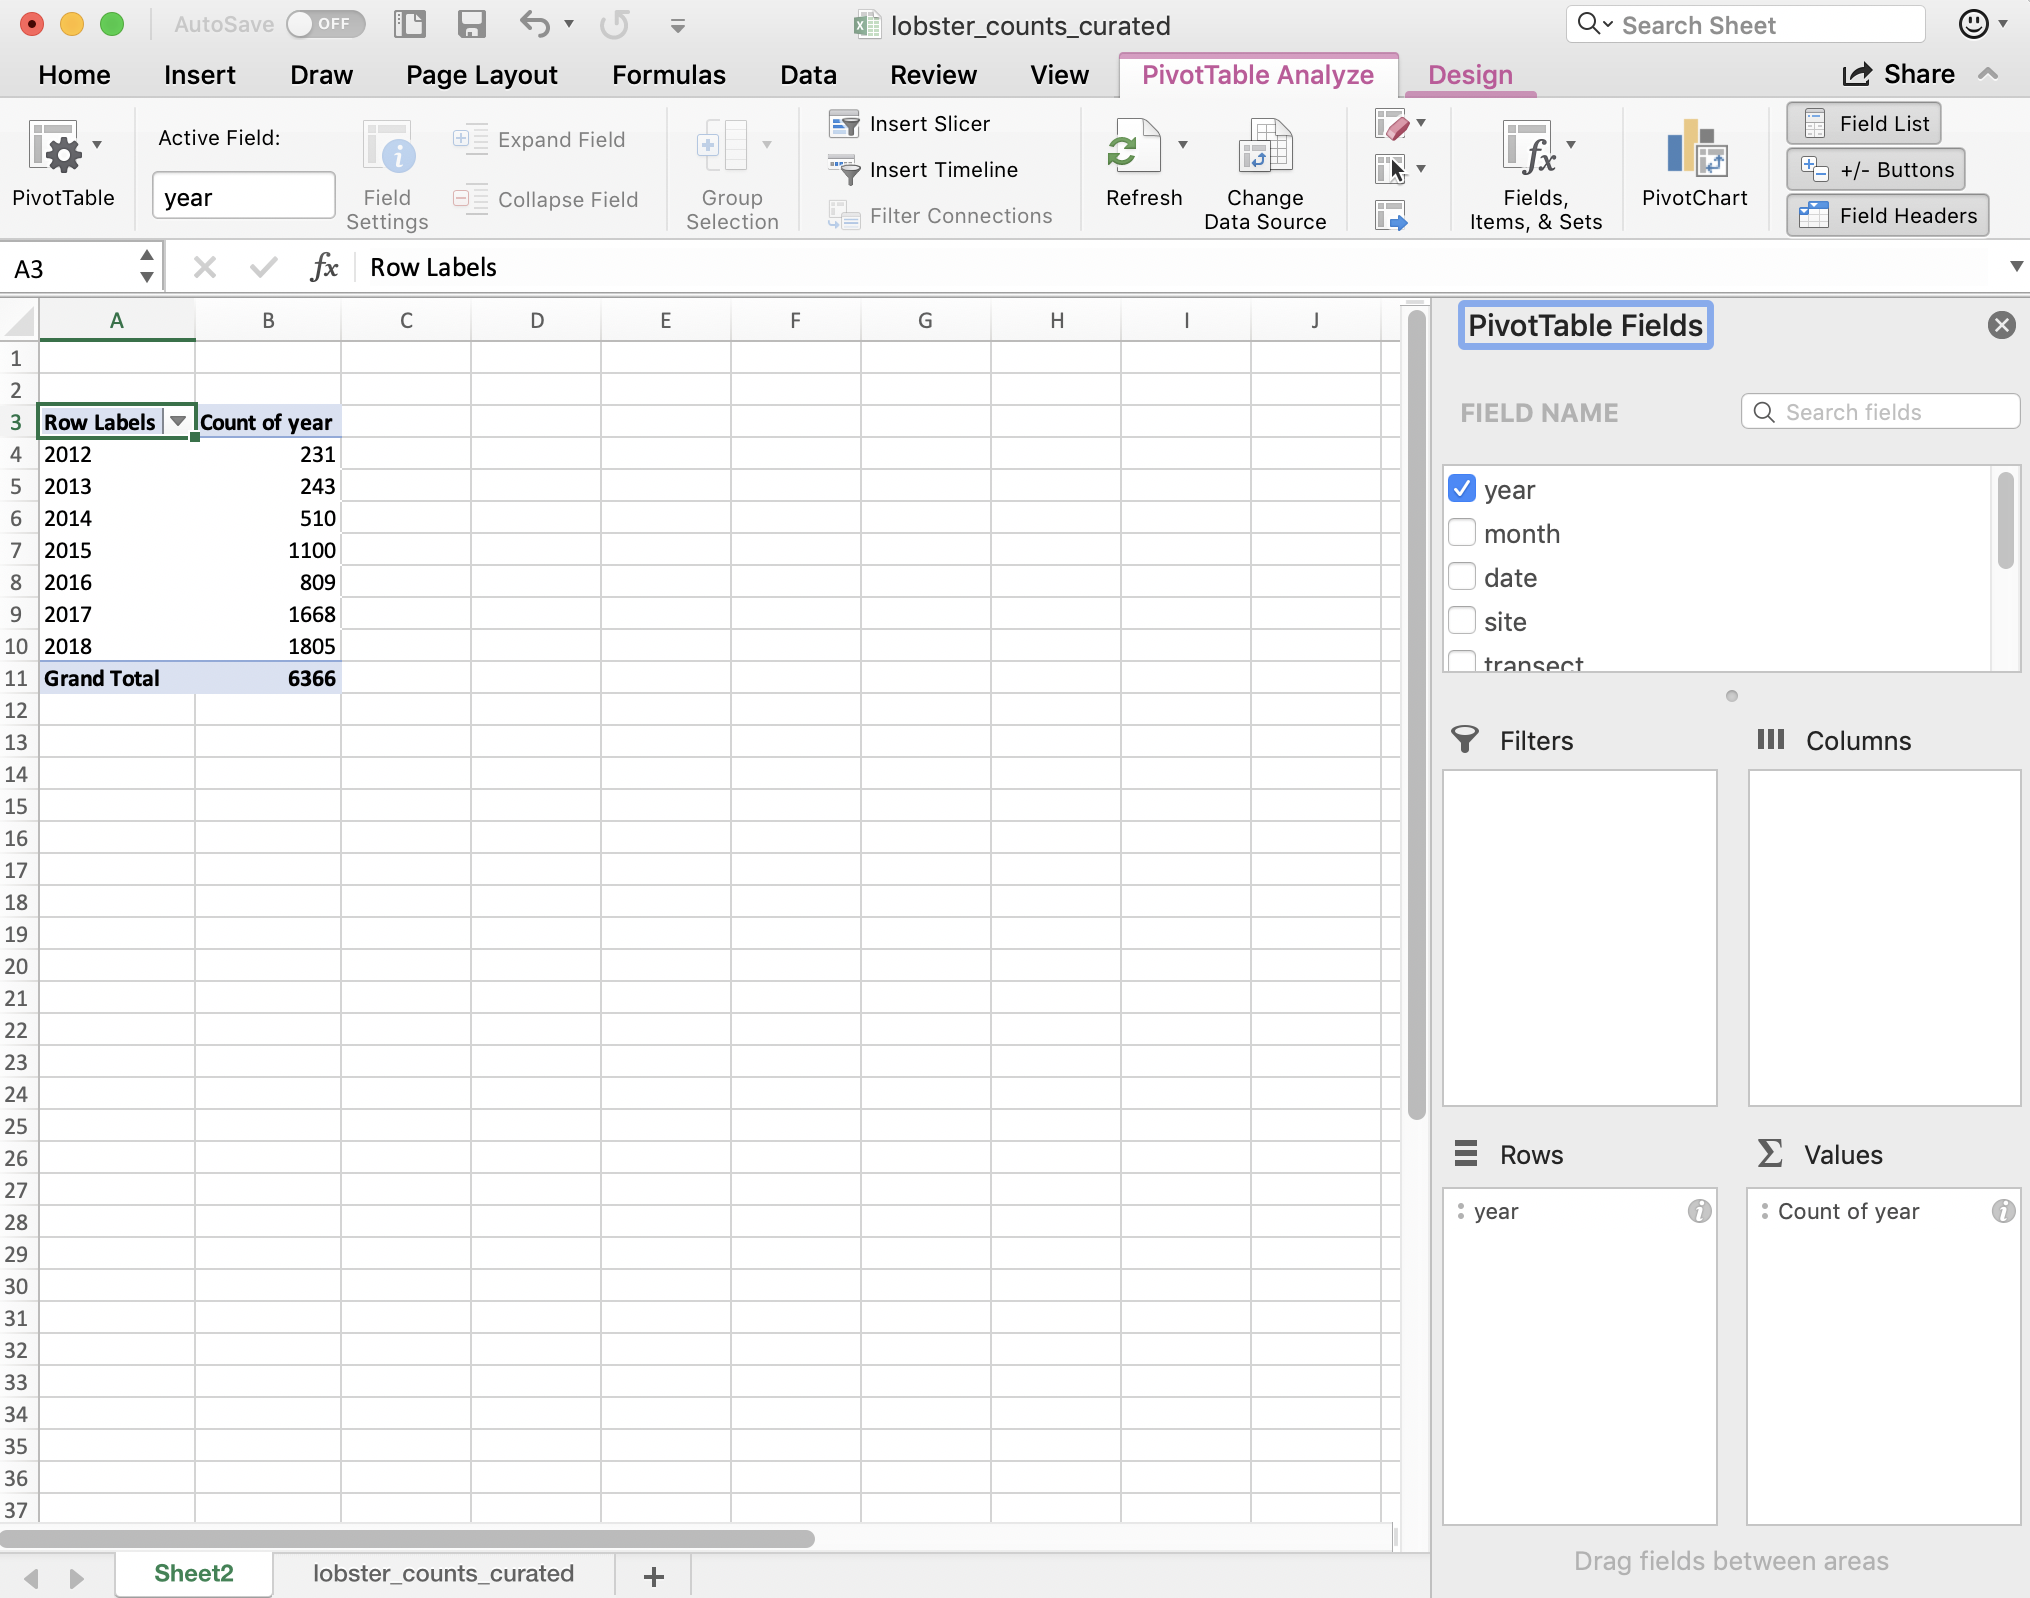
\includegraphics[width=0.6\linewidth]{img/pivot-table-count-year}

A few things to note:

\begin{itemize}
\tightlist
\item
  The pivot table is separate entity from our data (it's on a different sheet); the original data has not been affected
\item
  The pivot table only shows the variables we requested; we don't see other columns (like date, month, or site).
\end{itemize}

So pivot tables are great because they summarize the data and keep the raw data raw --- they even promote good pratice because they by default ask you if you'd like to present the data in a new sheet rather than in the same sheet.

\hypertarget{pivot-two-variables}{%
\subsection{pivot two variables}\label{pivot-two-variables}}

We can also add site as a second variable by dragging it:

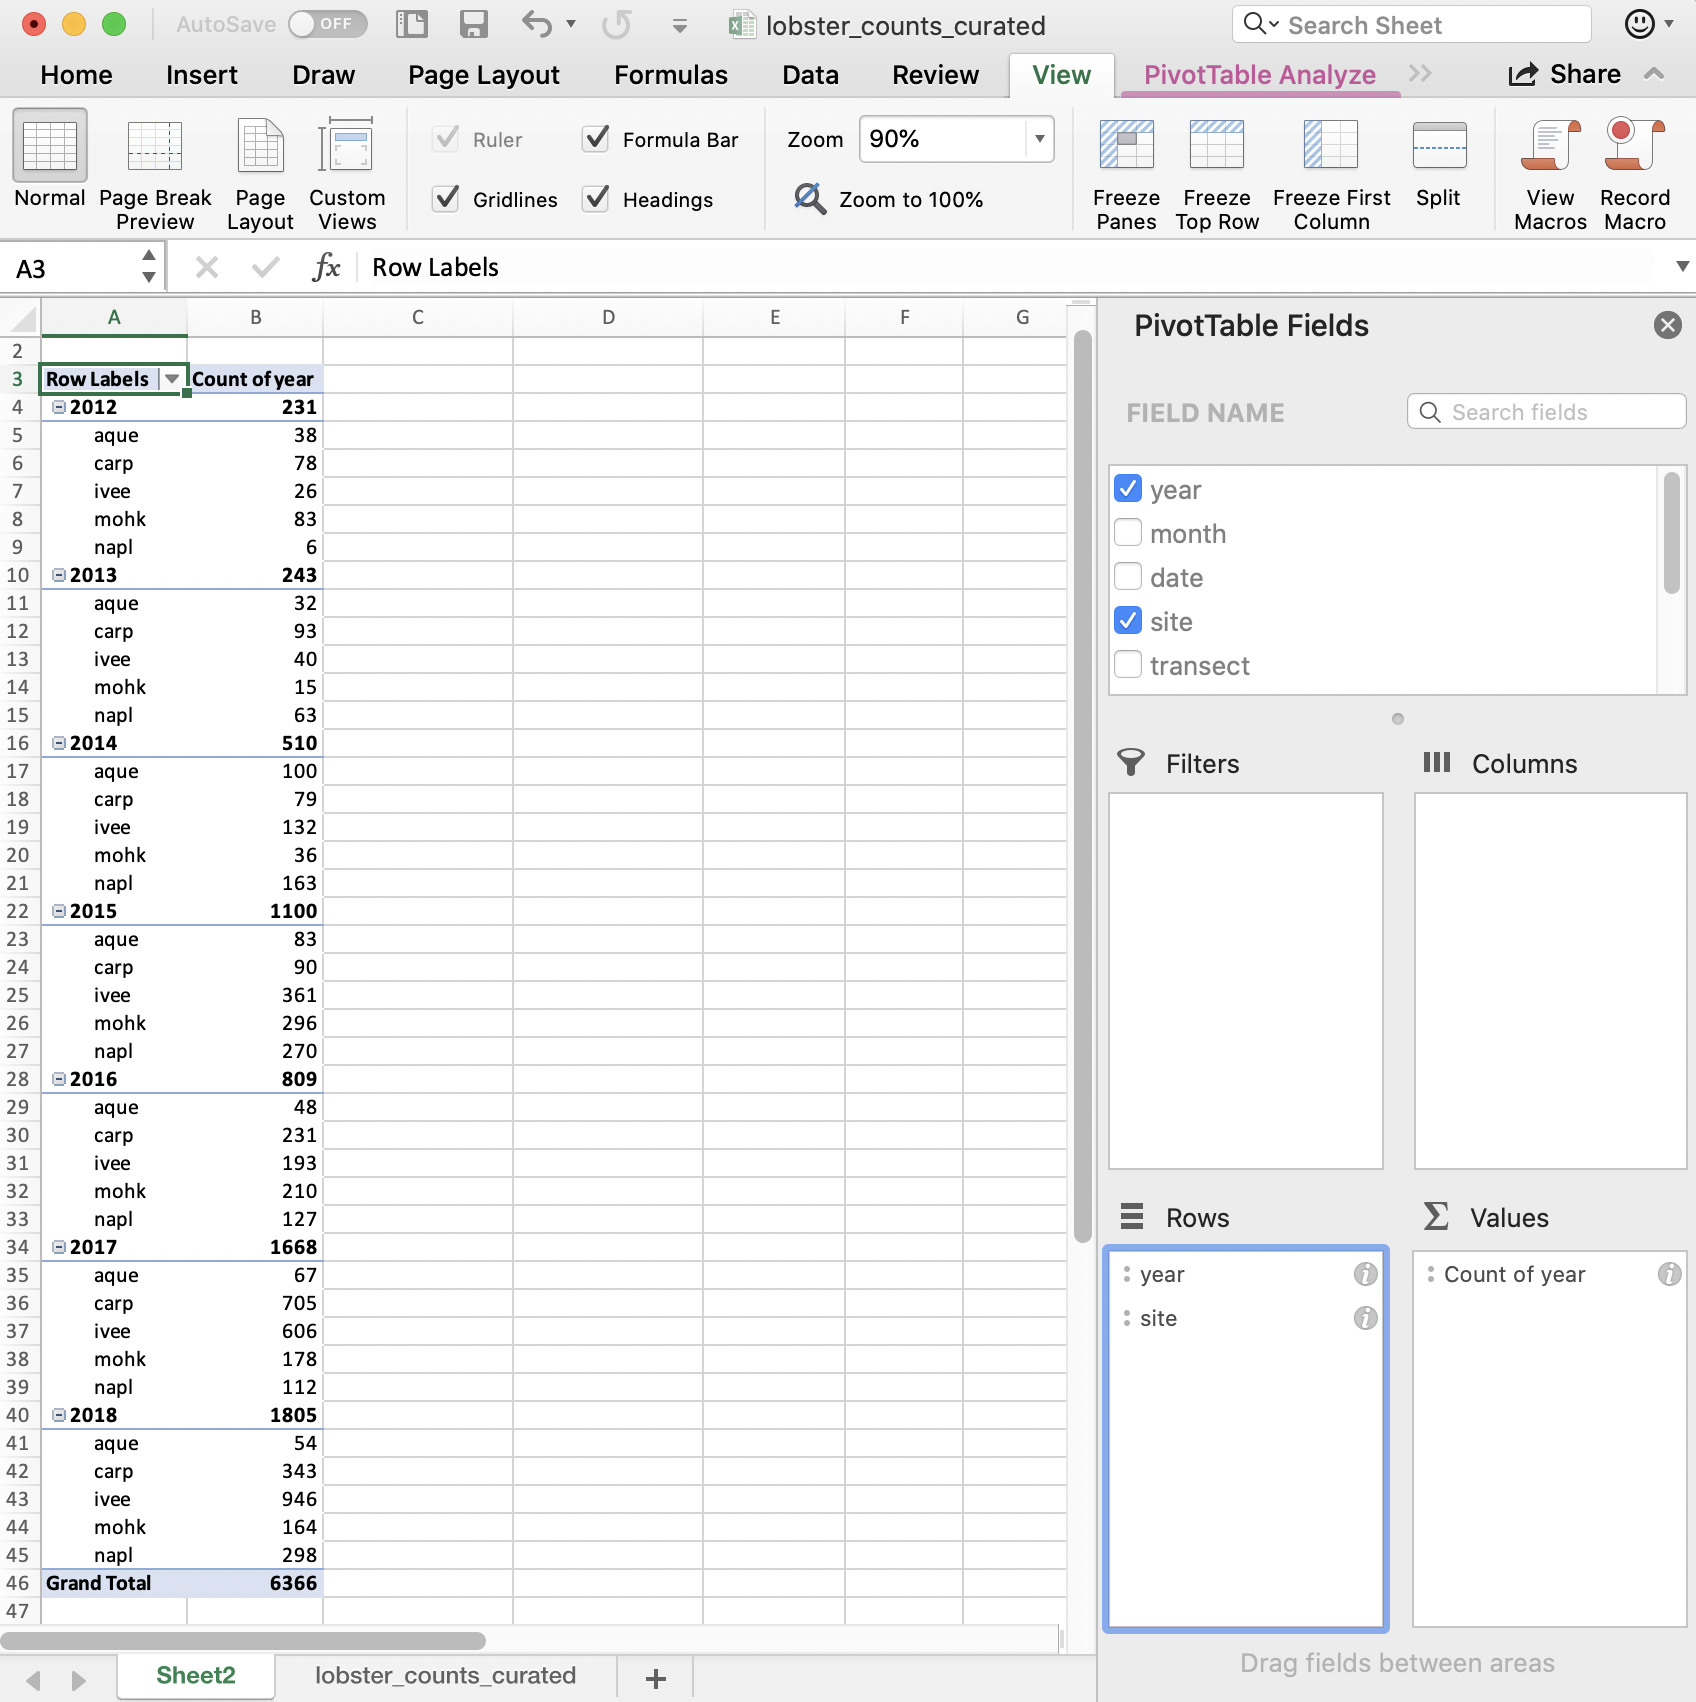
\includegraphics[width=0.6\linewidth]{img/pivot-table-count-year-site}

And then can reverse the order by dragging:

\includegraphics[width=0.6\linewidth]{img/pivot-table-count-site-year}

So in terms of our final interest of average size by site and year, we are on our way! I'm going to stop here because we want to be able to do this in R.

The power of R is in the automation, and in keeping that raw data truly raw.

Let's talk about how this looks like in R.

\hypertarget{group_by-summarize}{%
\section{\texorpdfstring{\texttt{group\_by()} \%\textgreater{}\% \texttt{summarize()}}{group\_by() \%\textgreater{}\% summarize()}}\label{group_by-summarize}}

In R, we can create the functionality of pivot tables by using 2 main \texttt{dplyr} verbs in combination: \texttt{group\_by} and \texttt{summarize}.

Say it with me: ``pivot tables are group\_by and then summarize''. And just like pivot tables, you have flexibility with how you are going to summarize. For example, we can calculate an average, or a total.

I think it's incredibly powerful to visualize what we are talking about with our data when do do these kinds of operations. It looks like this (from \href{http://www.rstudio.com/wp-content/uploads/2015/02/data-wrangling-cheatsheet.pdf}{RStudio's cheatsheet}; all cheatsheets available from \url{https://rstudio.com/resources/cheatsheets}):

\includegraphics[width=0.8\linewidth]{img/rstudio-cheatsheet-group_by_summarize}

When we were reporting by year or site, we were essentially modifying what we were grouping by (the different colors here in this figure.

Let's do this in R.

\hypertarget{group_by-one-variable}{%
\subsection{\texorpdfstring{\texttt{group\_by} one variable}{group\_by one variable}}\label{group_by-one-variable}}

Let's try this on our \texttt{lobsters} data, just like we did in Excel. We will count the the total number of lobster by year. In R vocabulary, we will group\_by year and then summarize by counting using \texttt{n()}, which is a function from \texttt{dplyr}. \texttt{n()} counts the number of times an observation shows up, and since this is uncounted data, this will count each row. We'll also use the pipe operator \texttt{\%\textgreater{}\%}, which you can read as ``and then''.

This to me reads: ``take the lobsters data and then group\_by year and then summarize by count in a new column called `count'\,''

\begin{Shaded}
\begin{Highlighting}[]
\NormalTok{lobsters }\OperatorTok
\StringTok{  }\KeywordTok{group_by}\NormalTok{(year) }\OperatorTok
\StringTok{  }\KeywordTok{summarize}\NormalTok{(}\DataTypeTok{count_by_year =} \KeywordTok{n}\NormalTok{())}
\end{Highlighting}
\end{Shaded}

\begin{verbatim}
## # A tibble: 5 x 2
##    year count_by_year
##   <dbl>         <int>
## 1  2012           231
## 2  2013           243
## 3  2014           510
## 4  2015          1100
## 5  2016           809
\end{verbatim}

Notice how together, \texttt{group\_by} and \texttt{summarize} minimize the amount of information we see. We also saw this with the pivot table. We lose the other columns that aren't involved here.

Question: What if you \emph{don't} group\_by first? Let's try it and discuss what's going on.

\begin{Shaded}
\begin{Highlighting}[]
\NormalTok{lobsters }\OperatorTok
\StringTok{  }\KeywordTok{summarize}\NormalTok{(}\DataTypeTok{count =}  \KeywordTok{n}\NormalTok{())}
\end{Highlighting}
\end{Shaded}

\begin{verbatim}
## # A tibble: 1 x 1
##   count
##   <int>
## 1  2893
\end{verbatim}

So if we don't \texttt{group\_by} first, we will get a single summary statistic (sum in this case) for the whole dataset.

Notice that in Excel we retain the overall totals for each site (in bold, on the same line with the site name). This is nice for communicating about data. But it can be problematic for further analyses, because it could be easy to take a total of this column and introduce errors.

\hypertarget{rstudio-viewer}{%
\subsection{RStudio Viewer}\label{rstudio-viewer}}

Let's now check the \texttt{lobsters} variable. We can do this by clicking on \texttt{lobsters} in the Environment pane in RStudio.

We see that we haven't changed any of our original data that was stored in this variable. (Just like how the pivot table didn't affect the raw data on the original sheet).

\begin{quote}
\textbf{\emph{Aside}}: You'll also see that when you click on the variable name in the Environment pane, \texttt{View(lobsters)} shows up in your Console. \texttt{View()} (capital V) is the R function to view any variable in the viewer. So this is something that you can write in your RMarkdown script, although RMarkdown will not be able to knit this view feature into the formatted document. So, if you want include \texttt{View()} in your RMarkdown document you will need to either comment it out \texttt{\#View()} or add \texttt{eval=FALSE} to the top of the code chunk so that the full line reads \texttt{\{r,\ eval=FALSE\}}.
\end{quote}

\hypertarget{group_by-multiple-variables}{%
\subsection{\texorpdfstring{\texttt{group\_by} multiple variables}{group\_by multiple variables}}\label{group_by-multiple-variables}}

Great. Now let's summarize by both year and site like we did in the pivot table. We are able to \texttt{group\_by} more than one variable. Let's do this together:

\begin{Shaded}
\begin{Highlighting}[]
\NormalTok{lobsters }\OperatorTok
\StringTok{  }\KeywordTok{group_by}\NormalTok{(site, year) }\OperatorTok
\StringTok{  }\KeywordTok{summarize}\NormalTok{(}\DataTypeTok{count_by_siteyear =}  \KeywordTok{n}\NormalTok{())}
\end{Highlighting}
\end{Shaded}

\begin{verbatim}
## # A tibble: 25 x 3
## # Groups:   site [5]
##    site   year count_by_siteyear
##    <chr> <dbl>             <int>
##  1 aque   2012                38
##  2 aque   2013                32
##  3 aque   2014               100
##  4 aque   2015                83
##  5 aque   2016                48
##  6 carp   2012                78
##  7 carp   2013                93
##  8 carp   2014                79
##  9 carp   2015                90
## 10 carp   2016               231
## # ... with 15 more rows
\end{verbatim}

text.

\hypertarget{summarize-multiple-variables}{%
\subsection{\texorpdfstring{\texttt{summarize} multiple variables}{summarize multiple variables}}\label{summarize-multiple-variables}}

We can summarize multiple variables at a time. So far we've done the count of lobster observations. Let's also do the mean and standard deviation. First let's use the \texttt{mean()} function to calculate the mean. We do this within the same summarize() function, but we can add a new line to make it easier to read. Notice how when you put your curser within the parenthesis and hit return, the indentation will automatically align.

\begin{Shaded}
\begin{Highlighting}[]
\NormalTok{lobsters }\OperatorTok
\StringTok{  }\KeywordTok{group_by}\NormalTok{(site, year) }\OperatorTok
\StringTok{  }\KeywordTok{summarize}\NormalTok{(}\DataTypeTok{count_by_siteyear =}  \KeywordTok{n}\NormalTok{(),}
            \DataTypeTok{mean_size_mm =} \KeywordTok{mean}\NormalTok{(size_mm))}
\end{Highlighting}
\end{Shaded}

\begin{verbatim}
## # A tibble: 25 x 4
## # Groups:   site [5]
##    site   year count_by_siteyear mean_size_mm
##    <chr> <dbl>             <int>        <dbl>
##  1 aque   2012                38         71  
##  2 aque   2013                32         72.1
##  3 aque   2014               100         76.9
##  4 aque   2015                83         68.5
##  5 aque   2016                48         68.7
##  6 carp   2012                78         74.4
##  7 carp   2013                93         76.6
##  8 carp   2014                79         NA  
##  9 carp   2015                90         70.7
## 10 carp   2016               231         68.9
## # ... with 15 more rows
\end{verbatim}

\begin{quote}
\textbf{\emph{Aside}} Command-I will properly indent selected lines.
\end{quote}

Great! But this will actually calculate some of the means as NA because one or more values in that year are NA. So we can pass an argument that says to remove NAs first before calculating the average. Let's do that, and then also calculate the standard deviation with the \texttt{sd()} function:

\begin{Shaded}
\begin{Highlighting}[]
\NormalTok{lobsters }\OperatorTok
\StringTok{  }\KeywordTok{group_by}\NormalTok{(site, year) }\OperatorTok
\StringTok{  }\KeywordTok{summarize}\NormalTok{(}\DataTypeTok{count_by_siteyear =}  \KeywordTok{n}\NormalTok{(), }
            \DataTypeTok{mean_size_mm =} \KeywordTok{mean}\NormalTok{(size_mm, }\DataTypeTok{na.rm=}\OtherTok{TRUE}\NormalTok{), }
            \DataTypeTok{sd_size_mm =} \KeywordTok{sd}\NormalTok{(size_mm, }\DataTypeTok{na.rm=}\OtherTok{TRUE}\NormalTok{))}
\end{Highlighting}
\end{Shaded}

\begin{verbatim}
## # A tibble: 25 x 5
## # Groups:   site [5]
##    site   year count_by_siteyear mean_size_mm sd_size_mm
##    <chr> <dbl>             <int>        <dbl>      <dbl>
##  1 aque   2012                38         71        10.2 
##  2 aque   2013                32         72.1      12.3 
##  3 aque   2014               100         76.9       9.32
##  4 aque   2015                83         68.5      12.6 
##  5 aque   2016                48         68.7      12.5 
##  6 carp   2012                78         74.4      14.6 
##  7 carp   2013                93         76.6       8.71
##  8 carp   2014                79         79.1       8.57
##  9 carp   2015                90         70.7      14.6 
## 10 carp   2016               231         68.9      12.5 
## # ... with 15 more rows
\end{verbatim}

So we can make the equivalent of Excel's pivot table in R with \texttt{group\_by} and then \texttt{summarize}. But a powerful thing about R is that maybe we want this information to be used in further analyses. We can make this easier for ourselves by saving this as a variable. So let's add a variable assignment to that first line:

\begin{Shaded}
\begin{Highlighting}[]
\NormalTok{siteyear_summary <-}\StringTok{ }\NormalTok{lobsters }\OperatorTok
\StringTok{  }\KeywordTok{group_by}\NormalTok{(site, year) }\OperatorTok
\StringTok{  }\KeywordTok{summarize}\NormalTok{(}\DataTypeTok{count_by_siteyear =}  \KeywordTok{n}\NormalTok{(), }
            \DataTypeTok{mean_size_mm =} \KeywordTok{mean}\NormalTok{(size_mm, }\DataTypeTok{na.rm =} \OtherTok{TRUE}\NormalTok{), }
            \DataTypeTok{sd_size_mm =} \KeywordTok{sd}\NormalTok{(size_mm, }\DataTypeTok{na.rm =} \OtherTok{TRUE}\NormalTok{))}

\NormalTok{siteyear_summary}
\end{Highlighting}
\end{Shaded}

\begin{verbatim}
## # A tibble: 25 x 5
## # Groups:   site [5]
##    site   year count_by_siteyear mean_size_mm sd_size_mm
##    <chr> <dbl>             <int>        <dbl>      <dbl>
##  1 aque   2012                38         71        10.2 
##  2 aque   2013                32         72.1      12.3 
##  3 aque   2014               100         76.9       9.32
##  4 aque   2015                83         68.5      12.6 
##  5 aque   2016                48         68.7      12.5 
##  6 carp   2012                78         74.4      14.6 
##  7 carp   2013                93         76.6       8.71
##  8 carp   2014                79         79.1       8.57
##  9 carp   2015                90         70.7      14.6 
## 10 carp   2016               231         68.9      12.5 
## # ... with 15 more rows
\end{verbatim}

\hypertarget{activity-2}{%
\subsection{Activity}\label{activity-2}}

Calculate the median \texttt{size\_mm} (Hint: ?median) and create a

Then, save, commit, and push your RMarkdown file.

Solution (no peeking):

\begin{Shaded}
\begin{Highlighting}[]
\NormalTok{siteyear_summary <-}\StringTok{ }\NormalTok{lobsters }\OperatorTok
\StringTok{  }\KeywordTok{group_by}\NormalTok{(site, year) }\OperatorTok
\StringTok{  }\KeywordTok{summarize}\NormalTok{(}\DataTypeTok{count_by_siteyear =}  \KeywordTok{n}\NormalTok{(), }
            \DataTypeTok{mean_size_mm =} \KeywordTok{mean}\NormalTok{(size_mm, }\DataTypeTok{na.rm =} \OtherTok{TRUE}\NormalTok{), }
            \DataTypeTok{sd_size_mm =} \KeywordTok{sd}\NormalTok{(size_mm, }\DataTypeTok{na.rm =} \OtherTok{TRUE}\NormalTok{), }
            \DataTypeTok{median_size_mm =} \KeywordTok{median}\NormalTok{(size_mm, }\DataTypeTok{na.rm =} \OtherTok{TRUE}\NormalTok{), )}

\NormalTok{siteyear_summary}

\CommentTok{## a ggplot option:}
\KeywordTok{ggplot}\NormalTok{(}\DataTypeTok{data =}\NormalTok{ siteyear_summary, }\KeywordTok{aes}\NormalTok{(}\DataTypeTok{x =}\NormalTok{ year, }\DataTypeTok{y =}\NormalTok{ median_size_mm, }\DataTypeTok{color =}\NormalTok{ site)) }\OperatorTok{+}
\StringTok{  }\KeywordTok{geom_line}\NormalTok{() }

\CommentTok{## another option:}
\KeywordTok{ggplot}\NormalTok{(siteyear_summary, }\KeywordTok{aes}\NormalTok{(}\DataTypeTok{x =}\NormalTok{ year, }\DataTypeTok{y =}\NormalTok{ median_size_mm)) }\OperatorTok{+}
\StringTok{  }\KeywordTok{geom_col}\NormalTok{() }\OperatorTok{+}
\StringTok{  }\KeywordTok{facet_wrap}\NormalTok{(}\OperatorTok{~}\NormalTok{site)}
\end{Highlighting}
\end{Shaded}

Don't forget to knit, commit, and push!

Nice work everybody.

\hypertarget{oh-no-our-colleague-sent-the-wrong-data}{%
\section{Oh no, our colleague sent the wrong data!}\label{oh-no-our-colleague-sent-the-wrong-data}}

Oh no! After all our analyses and everything we've done, our colleague just emailed us at 4:30pm on Friday that he sent the wrong data and we need to redo all our analyses with a new .xlsx file: \texttt{lobsters2.xlsx}, not \texttt{lobsters.xlsx}. Aaaaah!

If we were doing this in Excel, this would be a bummer; we'd have to rebuild our pivot table and click through all of our logic again.

But, since we did it in R, we are much safer. We can go back to the top of our RMarkdown file, and read in the updated dataset, and then re-knit. We will still need to check that everything outputs correctly, (and that column headers haven't been renamed), but our first pass will be to update the filename and re-knit:

\begin{Shaded}
\begin{Highlighting}[]
\CommentTok{## read in data}
\NormalTok{lobsters <-}\StringTok{ }\KeywordTok{read_xlsx}\NormalTok{(}\KeywordTok{here}\NormalTok{(}\StringTok{"data/lobsters2_curated.xlsx"}\NormalTok{))}
\end{Highlighting}
\end{Shaded}

And now we can see that our plot updated as well:

\begin{Shaded}
\begin{Highlighting}[]
\NormalTok{siteyear_summary <-}\StringTok{ }\NormalTok{lobsters }\OperatorTok
\StringTok{  }\KeywordTok{group_by}\NormalTok{(site, year) }\OperatorTok
\StringTok{  }\KeywordTok{summarize}\NormalTok{(}\DataTypeTok{count_by_siteyear =}  \KeywordTok{n}\NormalTok{(), }
            \DataTypeTok{mean_size_mm =} \KeywordTok{mean}\NormalTok{(size_mm, }\DataTypeTok{na.rm =} \OtherTok{TRUE}\NormalTok{), }
            \DataTypeTok{sd_size_mm =} \KeywordTok{sd}\NormalTok{(size_mm, }\DataTypeTok{na.rm =} \OtherTok{TRUE}\NormalTok{), }
            \DataTypeTok{median_size_mm =} \KeywordTok{median}\NormalTok{(size_mm, }\DataTypeTok{na.rm =} \OtherTok{TRUE}\NormalTok{), )}

\NormalTok{siteyear_summary}
\end{Highlighting}
\end{Shaded}

\begin{verbatim}
## # A tibble: 35 x 6
## # Groups:   site [5]
##    site   year count_by_siteyear mean_size_mm sd_size_mm median_size_mm
##    <chr> <dbl>             <int>        <dbl>      <dbl>          <dbl>
##  1 aque   2012                38         71        10.2            70  
##  2 aque   2013                32         72.1      12.3            75  
##  3 aque   2014               100         76.9       9.32           75.5
##  4 aque   2015                83         68.5      12.6            70  
##  5 aque   2016                48         68.7      12.5            71  
##  6 aque   2017                67         73.9      11.9            75  
##  7 aque   2018                54         71.7       8.14           72  
##  8 carp   2012                78         74.4      14.6            74.5
##  9 carp   2013                93         76.6       8.71           76  
## 10 carp   2014                79         79.1       8.57           79  
## # ... with 25 more rows
\end{verbatim}

\begin{Shaded}
\begin{Highlighting}[]
\CommentTok{## a ggplot option:}
\KeywordTok{ggplot}\NormalTok{(}\DataTypeTok{data =}\NormalTok{ siteyear_summary, }\KeywordTok{aes}\NormalTok{(}\DataTypeTok{x =}\NormalTok{ year, }\DataTypeTok{y =}\NormalTok{ median_size_mm, }\DataTypeTok{color =}\NormalTok{ site)) }\OperatorTok{+}
\StringTok{  }\KeywordTok{geom_line}\NormalTok{() }
\end{Highlighting}
\end{Shaded}

\includegraphics{R-for-Excel-Users_files/figure-latex/unnamed-chunk-93-1.pdf}

\begin{Shaded}
\begin{Highlighting}[]
\CommentTok{## another option:}
\KeywordTok{ggplot}\NormalTok{(siteyear_summary, }\KeywordTok{aes}\NormalTok{(}\DataTypeTok{x =}\NormalTok{ year, }\DataTypeTok{y =}\NormalTok{ median_size_mm)) }\OperatorTok{+}
\StringTok{  }\KeywordTok{geom_col}\NormalTok{() }\OperatorTok{+}
\StringTok{  }\KeywordTok{facet_wrap}\NormalTok{(}\OperatorTok{~}\NormalTok{site)}
\end{Highlighting}
\end{Shaded}

\includegraphics{R-for-Excel-Users_files/figure-latex/unnamed-chunk-93-2.pdf}

\hypertarget{dplyrcount}{%
\subsection{\texorpdfstring{\texttt{dplyr::count()}}{dplyr::count()}}\label{dplyrcount}}

Now that we've spent time with group\_by \%\textgreater{}\% summarize, there is a shortcut if you only want to summarize by count. This is with a function called \texttt{count()}, and it will group\_by your selected variable, count, and then also ungroup. It looks like this:

\begin{Shaded}
\begin{Highlighting}[]
\NormalTok{lobsters }\OperatorTok
\StringTok{  }\KeywordTok{count}\NormalTok{(site, year) }

\CommentTok{## This is the same as:}
\NormalTok{lobsters }\OperatorTok
\StringTok{  }\KeywordTok{group_by}\NormalTok{(site, year) }\OperatorTok\StringTok{ }
\StringTok{  }\KeywordTok{summarize}\NormalTok{(}\DataTypeTok{n =} \KeywordTok{n}\NormalTok{()) }\OperatorTok
\StringTok{  }\KeywordTok{ungroup}\NormalTok{()}
\end{Highlighting}
\end{Shaded}

Switching gears\ldots{}

\hypertarget{mutate}{%
\section{\texorpdfstring{\texttt{mutate()}}{mutate()}}\label{mutate}}

\includegraphics[width=0.8\linewidth]{img/rstudio-cheatsheet-mutate}

There are a lot of times where you don't want to summarize your data, but you do want to operate beyond the original data. This is often done by adding a column. We do this with the \texttt{mutate()} function from \texttt{dplyr}. Let's try this with our original lobsters data. The sizes are in millimeters but let's say it was important for them to be in meters. We can add a column with this calculation:

\begin{Shaded}
\begin{Highlighting}[]
\CommentTok{# quick reminder what this looks like}
\KeywordTok{head}\NormalTok{(lobsters)}
\end{Highlighting}
\end{Shaded}

\begin{verbatim}
## # A tibble: 6 x 7
##    year month date    site  transect replicate size_mm
##   <dbl> <dbl> <chr>   <chr>    <dbl> <chr>       <dbl>
## 1  2012     8 8/20/12 ivee         3 A              70
## 2  2012     8 8/20/12 ivee         3 B              60
## 3  2012     8 8/20/12 ivee         3 B              65
## 4  2012     8 8/20/12 ivee         3 B              70
## 5  2012     8 8/20/12 ivee         3 B              85
## 6  2012     8 8/20/12 ivee         3 C              60
\end{verbatim}

\begin{Shaded}
\begin{Highlighting}[]
\NormalTok{lobsters }\OperatorTok
\StringTok{  }\KeywordTok{mutate}\NormalTok{(}\DataTypeTok{size_m =}\NormalTok{ size_mm }\OperatorTok{/}\StringTok{ }\DecValTok{1000}\NormalTok{)}
\end{Highlighting}
\end{Shaded}

\begin{verbatim}
## # A tibble: 6,366 x 8
##     year month date    site  transect replicate size_mm size_m
##    <dbl> <dbl> <chr>   <chr>    <dbl> <chr>       <dbl>  <dbl>
##  1  2012     8 8/20/12 ivee         3 A              70  0.07 
##  2  2012     8 8/20/12 ivee         3 B              60  0.06 
##  3  2012     8 8/20/12 ivee         3 B              65  0.065
##  4  2012     8 8/20/12 ivee         3 B              70  0.07 
##  5  2012     8 8/20/12 ivee         3 B              85  0.085
##  6  2012     8 8/20/12 ivee         3 C              60  0.06 
##  7  2012     8 8/20/12 ivee         3 C              65  0.065
##  8  2012     8 8/20/12 ivee         3 C              67  0.067
##  9  2012     8 8/20/12 ivee         3 D              70  0.07 
## 10  2012     8 8/20/12 ivee         4 B              85  0.085
## # ... with 6,356 more rows
\end{verbatim}

If we want to add a column that has the same value repeated, we can pass it just one value, either a number or a character string (in quotes). And let's save this as a variable called \texttt{lobsters\_detailed}

\begin{Shaded}
\begin{Highlighting}[]
\NormalTok{lobsters_detailed <-}\StringTok{ }\NormalTok{lobsters }\OperatorTok
\StringTok{  }\KeywordTok{mutate}\NormalTok{(}\DataTypeTok{size_m =}\NormalTok{ size_mm }\OperatorTok{/}\StringTok{ }\DecValTok{1000}\NormalTok{, }
         \DataTypeTok{millenia =} \DecValTok{2000}\NormalTok{,}
         \DataTypeTok{observer =} \StringTok{"Allison Horst"}\NormalTok{)}
\end{Highlighting}
\end{Shaded}

\hypertarget{select}{%
\section{\texorpdfstring{\texttt{select()}}{select()}}\label{select}}

We will end with one final function, \texttt{select}. This is how to choose, retain, and move your data by columns:

\includegraphics[width=0.8\linewidth]{img/rstudio-cheatsheet-select}

Let's say that we want to present this data finally with only columns for date, site, and size in meters. We would do this:

\begin{Shaded}
\begin{Highlighting}[]
\NormalTok{lobsters_detailed }\OperatorTok
\StringTok{  }\KeywordTok{select}\NormalTok{(date, site, size_m)}
\end{Highlighting}
\end{Shaded}

\begin{verbatim}
## # A tibble: 6,366 x 3
##    date    site  size_m
##    <chr>   <chr>  <dbl>
##  1 8/20/12 ivee   0.07 
##  2 8/20/12 ivee   0.06 
##  3 8/20/12 ivee   0.065
##  4 8/20/12 ivee   0.07 
##  5 8/20/12 ivee   0.085
##  6 8/20/12 ivee   0.06 
##  7 8/20/12 ivee   0.065
##  8 8/20/12 ivee   0.067
##  9 8/20/12 ivee   0.07 
## 10 8/20/12 ivee   0.085
## # ... with 6,356 more rows
\end{verbatim}

One last time, let's knit, save, commit, and push to GitHub.

\hypertarget{deep-thoughts-2}{%
\section{Deep thoughts}\label{deep-thoughts-2}}

Highly recommended read: \href{https://peerj.com/preprints/3183/}{Broman \& Woo: Data organization in spreadsheets}. Practical tips to make spreadsheets less error-prone, easier for computers to process, easier to share

Great opening line: ``Spreadsheets, for all of their mundane rectangularness, have been the subject of angst and controversy for decades.''

\hypertarget{efficiency-tips-4}{%
\section{Efficiency Tips}\label{efficiency-tips-4}}

arrow keys with shift, option, command

\hypertarget{tidying}{%
\chapter{Tidying}\label{tidying}}

TODO: janitor: adorn and kable

\hypertarget{summary-5}{%
\section{Summary}\label{summary-5}}

In previous sessions, we learned to read in data, do some wrangling, and create a graph and table. Here, we'll continue by \emph{reshaping} data frames (converting from long-to-wide, or wide-to-long format), \emph{separating} and \emph{uniting} variable (column) contents, converting between \emph{explicit} and \emph{implicit} missing (\texttt{NA}) values, and cleaning up our column names with the \texttt{janitor} package.

\hypertarget{objectives-5}{%
\section{Objectives}\label{objectives-5}}

\begin{itemize}
\tightlist
\item
  Reshape data frames with \texttt{tidyr::pivot\_wider()} and \texttt{tidyr::pivot\_longer()}
\item
  Convert column names with \texttt{janitor::clean\_names()}
\item
  Combine or separate information from columns with \texttt{tidyr::unite()} and \texttt{tidyr::separate()}
\item
  Make implicit missings \emph{explicit} with \texttt{tidyr::complete()}
\item
  Make explicit missings \emph{implicit} with \texttt{tidyr::drop\_na()}
\item
  Use our new skills as part of a bigger wrangling sequence
\item
  Make a customized table (TODO: or introduce Kable if not time in pivot tables chapter)
\end{itemize}

\hypertarget{resources-6}{%
\section{Resources}\label{resources-6}}

-- \href{https://r4ds.had.co.nz/tidy-data.html}{Ch. 12 \emph{Tidy Data}, in R for Data Science} by Grolemund \& Wickham
- \href{https://tidyr.tidyverse.org/}{\texttt{tidyr} documentation from tidyverse.org}
- \href{https://github.com/sfirke/janitor}{\texttt{janitor} repo / information} from Sam Firke

\hypertarget{lesson-2}{%
\section{Lesson}\label{lesson-2}}

\hypertarget{lesson-prep}{%
\subsection{Lesson Prep}\label{lesson-prep}}

\hypertarget{create-a-new-r-markdown-and-attach-packages}{%
\subsubsection{Create a new R Markdown and attach packages}\label{create-a-new-r-markdown-and-attach-packages}}

Within your day 2 R Project, create a new .Rmd. Attach the \texttt{tidyverse}, \texttt{janitor} and \texttt{readxl} packages with \texttt{library(package\_name)}. Knit and save your new .Rmd within the project folder.

\begin{Shaded}
\begin{Highlighting}[]
\CommentTok{# Attach packages}
\KeywordTok{library}\NormalTok{(tidyverse)}
\KeywordTok{library}\NormalTok{(janitor)}
\KeywordTok{library}\NormalTok{(readxl)}
\end{Highlighting}
\end{Shaded}

\hypertarget{read-in-data}{%
\subsubsection{Read in data}\label{read-in-data}}

Use \texttt{readxl::read\_excel()} to import the ``invert\_counts\_curated.xlsx'' data:

\begin{Shaded}
\begin{Highlighting}[]
\NormalTok{inverts_df <-}\StringTok{ }\NormalTok{readxl}\OperatorTok{::}\KeywordTok{read_excel}\NormalTok{(}\StringTok{"invert_counts_curated.xlsx"}\NormalTok{)}
\end{Highlighting}
\end{Shaded}

Be sure to explore the imported data a bit:

\begin{itemize}
\tightlist
\item
  \texttt{View()}
\item
  \texttt{names()}
\item
  \texttt{summary()}
\end{itemize}

\hypertarget{reshaping-with-tidyrpivot_longer-and-tidyrpivot_wider}{%
\subsection{\texorpdfstring{Reshaping with \texttt{tidyr::pivot\_longer()} and \texttt{tidyr::pivot\_wider()}}{Reshaping with tidyr::pivot\_longer() and tidyr::pivot\_wider()}}\label{reshaping-with-tidyrpivot_longer-and-tidyrpivot_wider}}

\hypertarget{wide-to-longer-format-with-tidyrpivot_longer}{%
\subsubsection{\texorpdfstring{Wide-to-longer format with \texttt{tidyr::pivot\_longer()}}{Wide-to-longer format with tidyr::pivot\_longer()}}\label{wide-to-longer-format-with-tidyrpivot_longer}}

In \emph{tidy format}, each variable is contained within a single column. If we look at \emph{inverts\_df}, we can see that the \emph{year} variable is actually split over 3 columns, so we'd say this is currently in \textbf{wide format}.

There may be times when you want to have data in wide format, but often with code it is more efficient to convert to \textbf{long format} by gathering together observations for a variable that is currently split into multiple columns.

Schematically, converting from wide to long format looks like this:

\includegraphics{img/tidyr_pivot_longer.png}

Generally, the code to gather wide columns together using \texttt{tidyr::pivot\_longer()} looks like this:

TODO: Add pivot\_longer() schematic

We'll use \texttt{tidyr::pivot\_longer()} to gather data from all years in \emph{inverts\_df} into two columns: one called \emph{year}, which contains the year (as a number), and another called \emph{sp\_count} that contains the number of each species observed. The new data frame will be stored as \emph{inverts\_long}:

\begin{Shaded}
\begin{Highlighting}[]
\NormalTok{inverts_long <-}\StringTok{ }\NormalTok{tidyr}\OperatorTok{::}\KeywordTok{pivot_longer}\NormalTok{(}\DataTypeTok{data =}\NormalTok{ inverts_df, }
                                    \DataTypeTok{cols =} \StringTok{'2016'}\OperatorTok{:}\StringTok{'2018'}\NormalTok{,}
                                    \DataTypeTok{names_to =} \StringTok{"year"}\NormalTok{,}
                                    \DataTypeTok{values_to =} \StringTok{"sp_count"}\NormalTok{)}
\end{Highlighting}
\end{Shaded}

The outcome is the new long-format \emph{inverts\_long} data frame:

\begin{Shaded}
\begin{Highlighting}[]
\NormalTok{inverts_long}
\end{Highlighting}
\end{Shaded}

\begin{verbatim}
## # A tibble: 165 x 5
##    month site  common_name              year  sp_count
##    <chr> <chr> <chr>                    <chr>    <dbl>
##  1 7     abur  california cone snail    2016       451
##  2 7     abur  california cone snail    2017        28
##  3 7     abur  california cone snail    2018       762
##  4 7     abur  california spiny lobster 2016        17
##  5 7     abur  california spiny lobster 2017        17
##  6 7     abur  california spiny lobster 2018        16
##  7 7     abur  orange cup coral         2016        24
##  8 7     abur  orange cup coral         2017        24
##  9 7     abur  orange cup coral         2018        24
## 10 7     abur  purple urchin            2016        48
## # ... with 155 more rows
\end{verbatim}

Hooray, long format!

One thing that isn't obvious at first (but would become obvious if you continued working with this data) is that since those year numbers were initially column names (characters), when they are stacked into the \emph{year} column, their class wasn't auto-updated to numeric.

Explore the class of \emph{year} in \emph{inverts\_long}:

\begin{Shaded}
\begin{Highlighting}[]
\KeywordTok{class}\NormalTok{(inverts_long}\OperatorTok{$}\NormalTok{year)}
\end{Highlighting}
\end{Shaded}

\begin{verbatim}
## [1] "character"
\end{verbatim}

We'll use \texttt{dplyr::mutate()} in a different way here: to create a new column (that's how we've used \texttt{mutate()} previously) that has the same name of an existing column, in order to update and overwrite the existing column.

In this case, we'll \texttt{mutate()} to add a column called \emph{year}, which contains an \texttt{as.numeric()} version of the existing \emph{year} variable:

\begin{Shaded}
\begin{Highlighting}[]
\CommentTok{# Coerce "year" class to numeric: }

\NormalTok{inverts_long <-}\StringTok{ }\NormalTok{inverts_long }\OperatorTok\StringTok{ }
\StringTok{  }\KeywordTok{mutate}\NormalTok{(}\DataTypeTok{year =} \KeywordTok{as.numeric}\NormalTok{(year))}
\end{Highlighting}
\end{Shaded}

Checking the class again, we see that \emph{year} has been updated to a numeric variable:

\begin{Shaded}
\begin{Highlighting}[]
\KeywordTok{class}\NormalTok{(inverts_long}\OperatorTok{$}\NormalTok{year)}
\end{Highlighting}
\end{Shaded}

\begin{verbatim}
## [1] "numeric"
\end{verbatim}

\hypertarget{long-to-wider-format-with-tidyrpivot_wider}{%
\subsubsection{\texorpdfstring{Long-to-wider format with \texttt{tidyr::pivot\_wider()}}{Long-to-wider format with tidyr::pivot\_wider()}}\label{long-to-wider-format-with-tidyrpivot_wider}}

In the previous example, we had information spread over multiple columns that we wanted to \emph{gather}. Sometimes, we'll have data that we want to \emph{spread} over multiple columns.

For example, imagine that starting from \emph{inverts\_long} we want each species in the \emph{common\_name} column to exist as its \textbf{own column}. In that case, we would be converting from a longer to a wider format, and will use \texttt{tidyr::pivot\_wider()} as follows:

TODO: Add pivot\_wider() schematic

Specifically for our data, we write code to spread the \emph{common\_name} column as follows:

\begin{Shaded}
\begin{Highlighting}[]
\NormalTok{inverts_wide <-}\StringTok{ }\NormalTok{inverts_long }\OperatorTok\StringTok{ }
\StringTok{  }\NormalTok{tidyr}\OperatorTok{::}\KeywordTok{pivot_wider}\NormalTok{(}\DataTypeTok{names_from =}\NormalTok{ common_name, }
                     \DataTypeTok{values_from =}\NormalTok{ sp_count)}
\end{Highlighting}
\end{Shaded}

\begin{Shaded}
\begin{Highlighting}[]
\NormalTok{inverts_wide}
\end{Highlighting}
\end{Shaded}

\begin{verbatim}
## # A tibble: 33 x 8
##    month site   year `california con~ `california spi~ `orange cup cor~
##    <chr> <chr> <dbl>            <dbl>            <dbl>            <dbl>
##  1 7     abur   2016              451               17               24
##  2 7     abur   2017               28               17               24
##  3 7     abur   2018              762               16               24
##  4 7     ahnd   2016               27               16               24
##  5 7     ahnd   2017               24               16               24
##  6 7     ahnd   2018               24               16               24
##  7 7     aque   2016             4971               48             1526
##  8 7     aque   2017             1752               48             1623
##  9 7     aque   2018             2616               48             1859
## 10 7     bull   2016             1735               24               36
## # ... with 23 more rows, and 2 more variables: `purple urchin` <dbl>, `rock
## #   scallop` <dbl>
\end{verbatim}

We can see that now each \emph{species} has its own column (wider format). But also notice that those column headers (since they have spaces) might not be in the most coder-friendly format\ldots{}

\hypertarget{meet-the-janitor-package}{%
\subsubsection{\texorpdfstring{Meet the \texttt{janitor} package}{Meet the janitor package}}\label{meet-the-janitor-package}}

The \texttt{janitor} package by Sam Firke is a brilliant collection of functions for some quick data cleaning. We recommend that you explore the different functions it contains. Like:

\begin{itemize}
\tightlist
\item
  \texttt{janitor::clean\_names()}: update column headers to a case of your choosing
\item
  \texttt{janitor::get\_dupes()}: see all rows that are duplicates within variables you choose
\item
  \texttt{janitor::remove\_empty()}: remove empty rows and/or columns
\item
  \texttt{janitor::andorn\_*()}: jazz up frequency tables of counts (we'll return to this for a table example in TODO: Session 8)
\item
  \ldots{}and more!
\end{itemize}

Here, we'll use \texttt{janitor::clean\_names()} to convert all of our column headers to a more convenient case - the default is \textbf{lower\_snake\_case}, which means all spaces and symbols are replaced with an underscore (or a word describing the symbol), all characters are lowercase, and a few other nice adjustments.

For example, \texttt{janitor::clean\_names()} would update these nightmare column names into much nicer forms:

\begin{itemize}
\tightlist
\item
  \texttt{My...RECENT-income!} becomes \texttt{my\_recent\_income}
\item
  \texttt{SAMPLE2.!test1} becomes \texttt{sample2\_test1}
\item
  \texttt{ThisIsTheName} becomes \texttt{this\_is\_the\_name}
\item
  \texttt{2015} becomes \texttt{x2015}
\end{itemize}

If we wanted to then use these columns (which we probably would, since we created them), we could clean the names to get them into more coder-friendly lower\_snake\_case with \texttt{janitor::clean\_names()}:

\begin{Shaded}
\begin{Highlighting}[]
\NormalTok{inverts_wide <-}\StringTok{ }\NormalTok{inverts_wide }\OperatorTok\StringTok{ }
\StringTok{  }\NormalTok{janitor}\OperatorTok{::}\KeywordTok{clean_names}\NormalTok{()}
\end{Highlighting}
\end{Shaded}

\begin{Shaded}
\begin{Highlighting}[]
\KeywordTok{names}\NormalTok{(inverts_wide)}
\end{Highlighting}
\end{Shaded}

\begin{verbatim}
## [1] "month"                    "site"                    
## [3] "year"                     "california_cone_snail"   
## [5] "california_spiny_lobster" "orange_cup_coral"        
## [7] "purple_urchin"            "rock_scallop"
\end{verbatim}

And there are other options for the case, like:

\begin{itemize}
\tightlist
\item
  ``snake'' produces snake\_case
\item
  ``lower\_camel'' or ``small\_camel'' produces lowerCamel
\item
  ``upper\_camel'' or ``big\_camel'' produces UpperCamel
\item
  ``screaming\_snake'' or ``all\_caps'' produces ALL\_CAPS
\item
  ``lower\_upper'' produces lowerUPPER
\item
  ``upper\_lower'' produces UPPERlower
\end{itemize}

\hypertarget{combine-or-separate-information-in-columns-with-tidyrunite-and-tidyrseparate}{%
\subsection{\texorpdfstring{Combine or separate information in columns with \texttt{tidyr::unite()} and \texttt{tidyr::separate()}}{Combine or separate information in columns with tidyr::unite() and tidyr::separate()}}\label{combine-or-separate-information-in-columns-with-tidyrunite-and-tidyrseparate}}

Sometimes we'll want to \emph{separate} contents of a single column into multiple columns, or \emph{combine} entries from different columns into a single column.

For example, the following data frame has \emph{genus} and \emph{species} in separate columns:

id

genus

species

common\_name

1

Scorpaena

guttata

sculpin

2

Sebastes

miniatus

vermillion

We may want to combine the genus and species into a single column, \emph{scientific\_name}:

id

scientific\_name

common\_name

1

Scorpaena guttata

sculpin

2

Sebastes miniatus

vermillion

Or we may want to do the reverse (separate information from a single column into multiple columns). Here, we'll learn \texttt{tidyr::unite()} and \texttt{tidyr::separate()} to help us do both.

\hypertarget{tidyrunite-to-merge-information-from-separate-columns}{%
\subsubsection{\texorpdfstring{\texttt{tidyr::unite()} to merge information from separate columns}{tidyr::unite() to merge information from separate columns}}\label{tidyrunite-to-merge-information-from-separate-columns}}

Use \texttt{tidyr::unite()} to combine (paste) information from multiple columns into a single column (as for the scientific name example above)

\includegraphics{img/rstudio-cheatsheet-unite.png}

To demonstrate uniting information from separate columns, we'll make a single column that has the combined information from \emph{site} abbreviation and \emph{year} in \emph{inverts\_wide}.

We need to give \texttt{tidyr::unite()} several arguments:

\begin{itemize}
\tightlist
\item
  \textbf{data:} the data frame containing columns we want to combine (or pipe into the function from the data frame)
\item
  \textbf{col:} the name of the new ``united'' column
\item
  the \textbf{columns you are uniting}
\item
  \textbf{sep:} the symbol, value or character to put between the united information from each column
\end{itemize}

\begin{Shaded}
\begin{Highlighting}[]
\NormalTok{inverts_unite <-}\StringTok{ }\NormalTok{inverts_wide }\OperatorTok\StringTok{ }
\StringTok{  }\NormalTok{tidyr}\OperatorTok{::}\KeywordTok{unite}\NormalTok{(}\DataTypeTok{col =} \StringTok{"site_year"}\NormalTok{, }\CommentTok{# What to name the new united column}
               \KeywordTok{c}\NormalTok{(site, year), }\CommentTok{# The columns we'll unite (site, year)}
               \DataTypeTok{sep =} \StringTok{"_"}\NormalTok{) }\CommentTok{# How to separate the things we're uniting}
\end{Highlighting}
\end{Shaded}

\begin{verbatim}
## # A tibble: 6 x 7
##   month site_year california_cone~ california_spin~ orange_cup_coral
##   <chr> <chr>                <dbl>            <dbl>            <dbl>
## 1 7     abur_2016              451               17               24
## 2 7     abur_2017               28               17               24
## 3 7     abur_2018              762               16               24
## 4 7     ahnd_2016               27               16               24
## 5 7     ahnd_2017               24               16               24
## 6 7     ahnd_2018               24               16               24
## # ... with 2 more variables: purple_urchin <dbl>, rock_scallop <dbl>
\end{verbatim}

Try updating the separator from "\_" to ``\emph{hello!}'' to see what the outcome column contains.

\texttt{tidyr::unite()} can also combine information from \emph{more} than two columns. For example, to combine the \emph{site}, \emph{common\_name} and \emph{year} columns from \emph{inverts\_long}, we could use:

\begin{Shaded}
\begin{Highlighting}[]
\CommentTok{# Uniting more than 2 columns: }

\NormalTok{inverts_triple_unite <-}\StringTok{ }\NormalTok{inverts_long }\OperatorTok\StringTok{ }
\StringTok{  }\NormalTok{tidyr}\OperatorTok{::}\KeywordTok{unite}\NormalTok{(}\DataTypeTok{col =} \StringTok{"year_site_name"}\NormalTok{,}
               \KeywordTok{c}\NormalTok{(year, site, common_name),}
               \DataTypeTok{sep =} \StringTok{"-"}\NormalTok{)}
\end{Highlighting}
\end{Shaded}

\begin{Shaded}
\begin{Highlighting}[]
\KeywordTok{head}\NormalTok{(inverts_triple_unite)}
\end{Highlighting}
\end{Shaded}

\begin{verbatim}
## # A tibble: 6 x 3
##   month year_site_name                     sp_count
##   <chr> <chr>                                 <dbl>
## 1 7     2016-abur-california cone snail         451
## 2 7     2017-abur-california cone snail          28
## 3 7     2018-abur-california cone snail         762
## 4 7     2016-abur-california spiny lobster       17
## 5 7     2017-abur-california spiny lobster       17
## 6 7     2018-abur-california spiny lobster       16
\end{verbatim}

\hypertarget{tidyrseparate-to-separate-information-into-multiple-columns}{%
\subsubsection{\texorpdfstring{\texttt{tidyr::separate()} to separate information into multiple columns}{tidyr::separate() to separate information into multiple columns}}\label{tidyrseparate-to-separate-information-into-multiple-columns}}

While \texttt{tidyr::unite()} allows us to combine information from multiple columns, it's more likely that you'll \emph{start} with a single column that you want to split up into pieces.

For example, I might want to split up a column containing the \emph{genus} and \emph{species} (\emph{Scorpaena guttata}) into two separate columns (\emph{Scorpaena} \textbar{} \emph{guttata}), so that I can count how many \emph{Scorpaena} organisms exist in my dataset at the genus level.

Use \texttt{tidyr::separate()} to ``separate a character column into multiple columns using a regular expression separator.''

\includegraphics{img/rstudio-cheatsheet-separate.png}

Let's start again with \emph{inverts\_unite}, where we have combined the \emph{site} and \emph{year} into a single column called \emph{site\_year}. If we want to \textbf{separate} those, we can use:

\begin{Shaded}
\begin{Highlighting}[]
\NormalTok{inverts_sep <-}\StringTok{ }\NormalTok{inverts_triple_unite }\OperatorTok\StringTok{ }
\StringTok{  }\NormalTok{tidyr}\OperatorTok{::}\KeywordTok{separate}\NormalTok{(year_site_name, }\DataTypeTok{into =} \KeywordTok{c}\NormalTok{(}\StringTok{"my_year"}\NormalTok{, }\StringTok{"my_site_name"}\NormalTok{))}
\end{Highlighting}
\end{Shaded}

\begin{verbatim}
## Warning: Expected 2 pieces. Additional pieces discarded in 165 rows [1, 2, 3, 4,
## 5, 6, 7, 8, 9, 10, 11, 12, 13, 14, 15, 16, 17, 18, 19, 20, ...].
\end{verbatim}

What is that warning \texttt{Expected\ 2\ pieces...} telling us? If we take a look at the resulting data frame \emph{inverts\_sep}, we see that it only keeps the first \textbf{two} pieces, and gets rid of the third (name). Which is a bit concerning, because we rarely want to just throw away information in a data frame.

\begin{Shaded}
\begin{Highlighting}[]
\KeywordTok{head}\NormalTok{(inverts_sep)}
\end{Highlighting}
\end{Shaded}

\begin{verbatim}
## # A tibble: 6 x 4
##   month my_year my_site_name sp_count
##   <chr> <chr>   <chr>           <dbl>
## 1 7     2016    abur              451
## 2 7     2017    abur               28
## 3 7     2018    abur              762
## 4 7     2016    abur               17
## 5 7     2017    abur               17
## 6 7     2018    abur               16
\end{verbatim}

That's problematic. How can we make sure we're keeping as many different elements as exist in the united column?

We have a couple of options:

\begin{enumerate}
\def\labelenumi{\arabic{enumi}.}
\tightlist
\item
  Create the \emph{number} of columns that are needed to retain as many elements as exist (in this case, 3, but we only created two new columns in the example above)
\end{enumerate}

\begin{Shaded}
\begin{Highlighting}[]
\NormalTok{inverts_sep3 <-}\StringTok{ }\NormalTok{inverts_triple_unite }\OperatorTok\StringTok{ }
\StringTok{  }\NormalTok{tidyr}\OperatorTok{::}\KeywordTok{separate}\NormalTok{(year_site_name, }\DataTypeTok{into =} \KeywordTok{c}\NormalTok{(}\StringTok{"the_year"}\NormalTok{, }\StringTok{"the_site"}\NormalTok{, }\StringTok{"the_name"}\NormalTok{))}
\end{Highlighting}
\end{Shaded}

\begin{verbatim}
## Warning: Expected 3 pieces. Additional pieces discarded in 165 rows [1, 2, 3, 4,
## 5, 6, 7, 8, 9, 10, 11, 12, 13, 14, 15, 16, 17, 18, 19, 20, ...].
\end{verbatim}

Another warning. What is that about? Let's take a look at the resulting data frame and think about what's missing (what are the ``pieces discarded''?):

\begin{Shaded}
\begin{Highlighting}[]
\KeywordTok{head}\NormalTok{(inverts_sep3)}
\end{Highlighting}
\end{Shaded}

\begin{verbatim}
## # A tibble: 6 x 5
##   month the_year the_site the_name   sp_count
##   <chr> <chr>    <chr>    <chr>         <dbl>
## 1 7     2016     abur     california      451
## 2 7     2017     abur     california       28
## 3 7     2018     abur     california      762
## 4 7     2016     abur     california       17
## 5 7     2017     abur     california       17
## 6 7     2018     abur     california       16
\end{verbatim}

Aha! Only the \emph{first word} of the common name was retained, and anything else was trashed. We want to keep everything after the second dash in the new \emph{the\_name} column.

That's because the \textbf{default is \texttt{extra\ =\ "warn"}}, which means that if you have more pieces than columns you're separating into, it will populate the columns that have been allotted (in our case, just 3) then drop any additional information, giving you a warning that pieces have been dropped.

To keep the extra pieces that have been dropped, add the \texttt{extra\ =\ "merge"} argument within \texttt{tidyr::separate()} to override:

\begin{Shaded}
\begin{Highlighting}[]
\NormalTok{inverts_sep_all <-}\StringTok{ }\NormalTok{inverts_triple_unite }\OperatorTok\StringTok{ }
\StringTok{  }\KeywordTok{separate}\NormalTok{(year_site_name, }
           \DataTypeTok{into =} \KeywordTok{c}\NormalTok{(}\StringTok{"sample_year"}\NormalTok{, }\StringTok{"location"}\NormalTok{, }\StringTok{"sp_name"}\NormalTok{), }
           \DataTypeTok{extra =} \StringTok{"merge"}\NormalTok{)}
\end{Highlighting}
\end{Shaded}

No warning there about things being discarded. Explore \emph{inverts\_sep\_all}:

\begin{verbatim}
## # A tibble: 165 x 5
##    month sample_year location sp_name                  sp_count
##    <chr> <chr>       <chr>    <chr>                       <dbl>
##  1 7     2016        abur     california cone snail         451
##  2 7     2017        abur     california cone snail          28
##  3 7     2018        abur     california cone snail         762
##  4 7     2016        abur     california spiny lobster       17
##  5 7     2017        abur     california spiny lobster       17
##  6 7     2018        abur     california spiny lobster       16
##  7 7     2016        abur     orange cup coral               24
##  8 7     2017        abur     orange cup coral               24
##  9 7     2018        abur     orange cup coral               24
## 10 7     2016        abur     purple urchin                  48
## # ... with 155 more rows
\end{verbatim}

We see that the resulting data frame has split \emph{year\_site\_name} into three separate columns, \emph{sample\_year}, \emph{location}, and \emph{sp\_name}, but now everything after the second break (``-'') remains together in \emph{sp\_name} instead of dropping pieces following the third word.

\hypertarget{convert-between-explicit-and-implicit-missings-nas}{%
\subsection{\texorpdfstring{Convert between explicit and implicit missings (\texttt{NA}s)}{Convert between explicit and implicit missings (NAs)}}\label{convert-between-explicit-and-implicit-missings-nas}}

An \emph{explicit missing} is when every possible outcome actually appears in a data frame as a row, even if a variable of interest for that row is missing (\texttt{NA}).

Conversely, an \emph{implicit missing} is when an observation (row) does \emph{not} appear in the data frame because a variable of interest contains an \texttt{NA} missing value.

Consider the following data:

day

animal

food\_choice

Monday

eagle

fish

Monday

mountain lion

squirrel

Monday

toad

NA

Tuesday

eagle

fish

Tuesday

mountain lion

deer

Tuesday

toad

flies

Notice that the row for \textbf{toad} still appears in the dataset for \textbf{Tuesday}, despite having a missing food choice for that day. This is an \emph{explicit missing} because the row still appears in the data frame.

If that row was removed, the resulting dataset would look like this:

\begin{Shaded}
\begin{Highlighting}[]
\NormalTok{df_missings }\OperatorTok\StringTok{ }
\StringTok{  }\KeywordTok{drop_na}\NormalTok{(food_choice) }\OperatorTok\StringTok{ }
\StringTok{  }\KeywordTok{kable}\NormalTok{()}
\end{Highlighting}
\end{Shaded}

day

animal

food\_choice

Monday

eagle

fish

Monday

mountain lion

squirrel

Tuesday

eagle

fish

Tuesday

mountain lion

deer

Tuesday

toad

flies

\ldots{}and if your reaction is ``But then how do I know there's a toad from \textbf{MONDAY}?'', then you can see how it can be a bit risky to have \emph{implicit missings} instead of \emph{explicit missings}.

Whichever we choose, we can convert between the two forms using \texttt{tidyr::drop\_na()} or \texttt{tidyr::complete()}:

\begin{itemize}
\tightlist
\item
  \texttt{tidyr::drop\_na()}: removes observations (rows) that contain \texttt{NA} for variable(s) of interest
\item
  \texttt{tidyr::complete()}: turns implicit missing values into explicit missing values by completing a data frame with missing combinations of data
\end{itemize}

We'll use both here, starting with the \emph{inverts\_long} data frame we created above.

Looking through \emph{inverts\_long}, we'll see that there are \texttt{NA} observations for every species at site \textbf{bull} in 2018 - but those \texttt{NA} counts do show up. First, we'll use \texttt{tidyr::drop\_na()} to make those missings implicit (invisible) instead:

\begin{Shaded}
\begin{Highlighting}[]
\NormalTok{inverts_implicit_NA <-}\StringTok{ }\NormalTok{inverts_long }\OperatorTok\StringTok{ }
\StringTok{  }\KeywordTok{drop_na}\NormalTok{(sp_count)}
\end{Highlighting}
\end{Shaded}

See that now, the rows that contained an \texttt{NA} in the \emph{sp\_count} column from \emph{inverts\_long} have been removed.

WAIT, I want them back! We can ask R to create explicit missings (by identifying which combinations of groups currently don't appear in the data frame) using \texttt{tidyr::complete()}:

\begin{Shaded}
\begin{Highlighting}[]
\NormalTok{inverts_explicit_NA <-}\StringTok{ }\NormalTok{inverts_implicit_NA }\OperatorTok\StringTok{ }
\StringTok{  }\KeywordTok{complete}\NormalTok{(month, site, common_name, year)}
\end{Highlighting}
\end{Shaded}

Now you'll see \texttt{inverts\_explicit\_NA} has those 5 ``missing'' observations shown in the data frame.

\hypertarget{activities}{%
\subsection{Activities}\label{activities}}

TODO

\hypertarget{fun-facts-insights}{%
\subsection{Fun facts / insights}\label{fun-facts-insights}}

TODO

\hypertarget{vlookup}{%
\chapter{Dplyr and vlookups}\label{vlookup}}

\hypertarget{summary-6}{%
\section{Summary}\label{summary-6}}

In previous sessions, we've learned to do some basic wrangling and find summary information with functions in the \texttt{dplyr} package, which exists within the \texttt{tidyverse}. We've used:

\begin{itemize}
\tightlist
\item
  \texttt{count()} to get counts of observations for groupings we specify (or the reverse!)
\item
  \texttt{mutate()}: \textbf{add} a new column, while keeping the existing ones
\item
  \texttt{group\_by()}: let R know that \textbf{groups} exist within the dataset, by variable(s)
\item
  \texttt{summarize()}: calculate a value (that you specify) for each group, then report each group's value in a table
\end{itemize}

In this session, we'll expand our data wrangling toolkit using:

\begin{itemize}
\tightlist
\item
  \texttt{filter()} to conditionally subset our data by \textbf{rows}, and
\item
  \texttt{*\_join()} functions to merge data frames together
\end{itemize}

The combination of \texttt{filter()} and \texttt{*\_join()} - to return rows satisfying a condition we specify, and merging data frames by like variables - is analogous to the useful VLOOKUP function in Excel.

\hypertarget{objectives-6}{%
\subsection{Objectives}\label{objectives-6}}

\begin{itemize}
\tightlist
\item
  Continue building R Markdown skills
\item
  Return \textbf{rows} that satisfy variable conditions using \texttt{filter()}
\item
  Use \texttt{full\_join()}, \texttt{left\_join()}, and \texttt{inner\_join()} to merge data frames by matching variables, with different endpoints in mind
\item
  Use \texttt{anti\_join()} to find things that \textbf{do not} exist in both data frames
\item
  Understand the similarities between \texttt{filter()} + \texttt{*\_join()} and Excel's VLOOKUP function
\end{itemize}

\hypertarget{resources-7}{%
\subsection{Resources}\label{resources-7}}

\begin{itemize}
\tightlist
\item
  \href{https://dplyr.tidyverse.org/reference/filter.html}{\texttt{filter()} documentation from tidyverse.org}
\item
  \href{https://dplyr.tidyverse.org/reference/join.html}{\texttt{join()} documentation from tidyverse.org}
\item
  \href{https://r4ds.had.co.nz/}{Chapters 5 and 13 in \emph{R for Data Science} by Garrett Grolemund and Hadley Wickham}
\end{itemize}

\hypertarget{lessons}{%
\section{Lessons}\label{lessons}}

\textbf{Session 5 set-up:} TODO

\begin{itemize}
\tightlist
\item
  Create a new .Rmd in your r-workshop directory (project)
\item
  Add some descriptive text
\item
  Add new code chunks to:

  \begin{itemize}
  \tightlist
  \item
    Attach packages
  \item
    Read in the necessary data
  \end{itemize}
\end{itemize}

In this session we'll use the \textbf{fish\_counts\_curated.csv} and \textbf{invert\_counts\_curated.xlsx} files, and the first worksheet from \textbf{kelp\_counts\_curated.xlsx}.

\begin{Shaded}
\begin{Highlighting}[]
\CommentTok{# Attach packages:}
\KeywordTok{library}\NormalTok{(tidyverse)}
\KeywordTok{library}\NormalTok{(readxl)}

\CommentTok{# Read in data: }
\NormalTok{invert_counts <-}\StringTok{ }\KeywordTok{read_excel}\NormalTok{(}\KeywordTok{here}\NormalTok{(}\StringTok{"data"}\NormalTok{, }\StringTok{"invert_counts_curated.xlsx"}\NormalTok{))}
\NormalTok{fish_counts <-}\StringTok{ }\KeywordTok{read_csv}\NormalTok{(}\KeywordTok{here}\NormalTok{(}\StringTok{"data"}\NormalTok{, }\StringTok{"fish_counts_curated.csv"}\NormalTok{))}
\NormalTok{kelp_counts_abur <-}\StringTok{ }\KeywordTok{read_excel}\NormalTok{(}\KeywordTok{here}\NormalTok{(}\StringTok{"data"}\NormalTok{, }\StringTok{"kelp_counts_curated.xlsx"}\NormalTok{))}
\end{Highlighting}
\end{Shaded}

Remember to always explore the data you've read in using functions like \texttt{View()}, \texttt{names()}, \texttt{summary()}, \texttt{head()} and \texttt{tail()} to ensure that the data you \emph{think} you read in is \emph{actually} the data you read in.

Now, let's use \texttt{filter()} to decide which observations (rows) we'll keep or exclude in new subsets, similar to using Excel's VLOOKUP function.

\hypertarget{filter-to-conditionally-subset-by-rows}{%
\subsection{\texorpdfstring{\texttt{filter()} to conditionally subset by rows}{filter() to conditionally subset by rows}}\label{filter-to-conditionally-subset-by-rows}}

Use \texttt{filter()} to let R know which \textbf{rows} you want to keep or exclude, based whether or not their contents match conditions that you set for one or more variables.

\includegraphics{img/rstudio-cheatsheet-filter.png}

Some examples in words that might inspire you to use \texttt{filter()}:

\begin{itemize}
\tightlist
\item
  ``I only want to keep rows where the temperature is greater than 90°F.''
\item
  ``I want to keep all observations \textbf{except} those where the tree type is listed as \textbf{unknown}.''
\item
  ``I want to make a new subset with only data for mountain lions (the species variable) in California (the state variable).''
\end{itemize}

When we use \texttt{filter()}, we need to let R know a couple of things:

\begin{itemize}
\tightlist
\item
  What data frame we're filtering from
\item
  What condition(s) we want observations to \textbf{match} and/or \textbf{not match} in order to keep them in the new subset
\end{itemize}

Follow along with the examples below to learn some common ways to use \texttt{filter()}.

\hypertarget{filter-rows-by-matching-a-single-character-string}{%
\subsubsection{Filter rows by matching a single character string}\label{filter-rows-by-matching-a-single-character-string}}

Let's say we want to keep all observations from the fish\_counts data frame where the common name is ``garibaldi.'' Here, we need to tell R to only \emph{keep rows} from the \textbf{fish\_counts} data frame when the common name (\textbf{common\_name} variable) exactly matches \textbf{garibaldi}.
Use \texttt{==} to ask R to look for matching strings:

\begin{Shaded}
\begin{Highlighting}[]
\NormalTok{fish_gari <-}\StringTok{ }\KeywordTok{filter}\NormalTok{(fish_counts, common_name }\OperatorTok{==}\StringTok{ "garibaldi"}\NormalTok{)}
\end{Highlighting}
\end{Shaded}

Check out the \textbf{fish\_gari} object to ensure that only \emph{garibaldi} observations remain.

You could also do this using the pipe operator \texttt{\%\textgreater{}\%} (though for a single function, it doesn't save much effort or typing):

\begin{Shaded}
\begin{Highlighting}[]
\NormalTok{fish_gari <-}\StringTok{ }\NormalTok{fish_counts }\OperatorTok\StringTok{ }
\StringTok{  }\KeywordTok{filter}\NormalTok{(common_name }\OperatorTok{==}\StringTok{ "garibaldi"}\NormalTok{)}
\end{Highlighting}
\end{Shaded}

\hypertarget{filter-rows-based-on-numeric-conditions}{%
\subsubsection{Filter rows based on numeric conditions}\label{filter-rows-based-on-numeric-conditions}}

Use expected operators (\textgreater{}, \textless{}, \textgreater{}=, \textless{}=, ==) to set conditions for a numeric variable when filtering. For this example, we only want to retain observations when the \textbf{total\_count} column value is \textgreater{}= 50:

\begin{Shaded}
\begin{Highlighting}[]
\NormalTok{fish_over50 <-}\StringTok{ }\KeywordTok{filter}\NormalTok{(fish_counts, total_count }\OperatorTok{>=}\StringTok{ }\DecValTok{50}\NormalTok{)}
\end{Highlighting}
\end{Shaded}

Or, using the pipe:

\begin{Shaded}
\begin{Highlighting}[]
\NormalTok{fish_over50 <-}\StringTok{ }\NormalTok{fish_counts }\OperatorTok\StringTok{ }
\StringTok{  }\KeywordTok{filter}\NormalTok{(total_count }\OperatorTok{>=}\StringTok{ }\DecValTok{50}\NormalTok{)}
\end{Highlighting}
\end{Shaded}

TODO: show example of between and exact =

\hypertarget{filter-to-return-rows-that-match-this-or-that-or-that}{%
\subsubsection{\texorpdfstring{Filter to return rows that match \emph{this} OR \emph{that} OR \emph{that}}{Filter to return rows that match this OR that OR that}}\label{filter-to-return-rows-that-match-this-or-that-or-that}}

What if we want to return a subset of the fish\_counts df that contains \emph{garibaldi}, \emph{blacksmith} OR \emph{black surfperch}?

There are several ways to write an ``OR'' statement for filtering, which will keep any observations that match Condition A \emph{or} Condition B \emph{or} Condition C. In this example, we will create a subset from \textbf{fish\_counts} that only contains rows where the \textbf{common\_name} is \emph{garibaldi} or \emph{blacksmith} or \emph{black surfperch}.

Use \texttt{\%in\%} to ask R to look for \emph{any matches} within a combined vector of strings:

\begin{Shaded}
\begin{Highlighting}[]
\NormalTok{fish_3sp <-}\StringTok{ }\NormalTok{fish_counts }\OperatorTok\StringTok{ }
\StringTok{  }\KeywordTok{filter}\NormalTok{(common_name }\OperatorTok\StringTok{ }\KeywordTok{c}\NormalTok{(}\StringTok{"garibaldi"}\NormalTok{, }\StringTok{"blacksmith"}\NormalTok{, }\StringTok{"black surfperch"}\NormalTok{))}
\end{Highlighting}
\end{Shaded}

Alternatively, you can indicate \textbf{OR} using the vertical line operator \texttt{\textbar{}} to do the same thing (but you can see that it's more repetitive when looking for matches within the same variable):

\begin{Shaded}
\begin{Highlighting}[]
\NormalTok{fish_3sp <-}\StringTok{ }\NormalTok{fish_counts }\OperatorTok\StringTok{ }
\StringTok{  }\KeywordTok{filter}\NormalTok{(common_name }\OperatorTok{==}\StringTok{ "garibaldi"} \OperatorTok{|}\StringTok{ }\NormalTok{common_name }\OperatorTok{==}\StringTok{ "blacksmith"} \OperatorTok{|}\StringTok{ }\NormalTok{common_name }\OperatorTok{==}\StringTok{ "black surfperch"}\NormalTok{)}
\end{Highlighting}
\end{Shaded}

\hypertarget{filter-to-return-rows-that-match-conditions-for-multiple-variables}{%
\subsubsection{Filter to return rows that match conditions for multiple variables}\label{filter-to-return-rows-that-match-conditions-for-multiple-variables}}

In the previous examples, we set filter conditions based on a single variable (e.g.~common\_name). What if we want to return observations that satisfy conditions for multiple variables?

For example: We want to create a subset that only returns rows from `invert\_counts' where the \textbf{site} is ``abur'' or ``mohk'' \emph{and} the \textbf{common\_name} is ``purple urchin.'' In \texttt{filter()}, add a comma (or ampersand, \&) between arguments for multiple \emph{AND} conditions:

\begin{Shaded}
\begin{Highlighting}[]
\NormalTok{urchin_abur_mohk <-}\StringTok{ }\NormalTok{invert_counts }\OperatorTok\StringTok{ }
\StringTok{  }\KeywordTok{filter}\NormalTok{(site }\OperatorTok\StringTok{ }\KeywordTok{c}\NormalTok{(}\StringTok{"abur"}\NormalTok{,}\StringTok{"mohk"}\NormalTok{), common_name }\OperatorTok{==}\StringTok{ "purple urchin"}\NormalTok{)}
\end{Highlighting}
\end{Shaded}

\begin{Shaded}
\begin{Highlighting}[]
\KeywordTok{head}\NormalTok{(urchin_abur_mohk)}
\end{Highlighting}
\end{Shaded}

\begin{verbatim}
## # A tibble: 2 x 6
##   month site  common_name   `2016` `2017` `2018`
##   <chr> <chr> <chr>          <dbl>  <dbl>  <dbl>
## 1 7     abur  purple urchin     48     48     48
## 2 7     mohk  purple urchin    620    505    323
\end{verbatim}

Like most things in R, there are other ways to do the same thing. For example, you could do the same thing using \texttt{\&} (instead of a comma) between ``and'' conditions:

\begin{Shaded}
\begin{Highlighting}[]
\CommentTok{# Use the ampersand (&) to add another condition "and this must be true":}

\NormalTok{urchin_abur_mohk <-}\StringTok{ }\NormalTok{invert_counts }\OperatorTok\StringTok{ }
\StringTok{  }\KeywordTok{filter}\NormalTok{(site }\OperatorTok\StringTok{ }\KeywordTok{c}\NormalTok{(}\StringTok{"abur"}\NormalTok{,}\StringTok{"mohk"}\NormalTok{) }\OperatorTok{&}\StringTok{ }\NormalTok{common_name }\OperatorTok{==}\StringTok{ "purple urchin"}\NormalTok{)}
\end{Highlighting}
\end{Shaded}

Or you could just do two filter steps in sequence:

\begin{Shaded}
\begin{Highlighting}[]
\CommentTok{# Written as multiple filter steps:}

\NormalTok{urchin_abur_mohk <-}\StringTok{ }\NormalTok{invert_counts }\OperatorTok\StringTok{ }
\StringTok{  }\KeywordTok{filter}\NormalTok{(site }\OperatorTok\StringTok{ }\KeywordTok{c}\NormalTok{(}\StringTok{"abur"}\NormalTok{, }\StringTok{"mohk"}\NormalTok{)) }\OperatorTok\StringTok{ }
\StringTok{  }\KeywordTok{filter}\NormalTok{(common_name }\OperatorTok{==}\StringTok{ "purple urchin"}\NormalTok{)}
\end{Highlighting}
\end{Shaded}

\hypertarget{filter-to-return-rows-that-do-not-match-conditions}{%
\subsubsection{\texorpdfstring{Filter to return rows that \emph{do not} match conditions}{Filter to return rows that do not match conditions}}\label{filter-to-return-rows-that-do-not-match-conditions}}

Sometimes we might want to exclude observations. Here, let's say we want to make a subset that contains all rows from \textbf{fish\_counts} except those recorded at the Mohawk Reef site (``mohk'' in the \emph{site} variable).

We use \texttt{!=} to return observations that \textbf{do not match} a condition.

Like this:

\begin{Shaded}
\begin{Highlighting}[]
\NormalTok{fish_no_mohk <-}\StringTok{ }\NormalTok{fish_counts }\OperatorTok\StringTok{ }
\StringTok{  }\KeywordTok{filter}\NormalTok{(site }\OperatorTok{!=}\StringTok{ "mohk"}\NormalTok{)}
\end{Highlighting}
\end{Shaded}

This similarly works to exclude observations by a value.

For example, if we want to return all observations \emph{except} those where the total fish count is 1, we use:

\begin{Shaded}
\begin{Highlighting}[]
\NormalTok{fish_more_one <-}\StringTok{ }\NormalTok{fish_counts }\OperatorTok\StringTok{ }
\StringTok{  }\KeywordTok{filter}\NormalTok{(total_count }\OperatorTok{!=}\StringTok{ }\DecValTok{1}\NormalTok{)}
\end{Highlighting}
\end{Shaded}

What if we want to exclude observations for multiple conditions? For example, here we want to return all rows where the fish species \textbf{is not} garibaldi \textbf{or} rock wrasse.

We can use \texttt{filter(!variable\ \%in\%\ c("apple",\ "orange"))} to return rows where the variable does \textbf{not} match ``apple'' or ``orange''. For our fish example, that looks like this:

\begin{Shaded}
\begin{Highlighting}[]
\NormalTok{fish_subset <-}\StringTok{ }\NormalTok{fish_counts }\OperatorTok\StringTok{ }
\StringTok{  }\KeywordTok{filter}\NormalTok{(}\OperatorTok{!}\NormalTok{common_name }\OperatorTok\StringTok{ }\KeywordTok{c}\NormalTok{(}\StringTok{"garibaldi"}\NormalTok{, }\StringTok{"rock wrasse"}\NormalTok{))}
\end{Highlighting}
\end{Shaded}

Which then only returns observations for the other fish species in the dataset.

\begin{Shaded}
\begin{Highlighting}[]
\KeywordTok{head}\NormalTok{(fish_subset)}
\end{Highlighting}
\end{Shaded}

\begin{verbatim}
## # A tibble: 6 x 4
##    year site  common_name     total_count
##   <dbl> <chr> <chr>                 <dbl>
## 1  2016 abur  black surfperch           2
## 2  2016 abur  blacksmith                1
## 3  2016 abur  senorita                 58
## 4  2016 aque  black surfperch           1
## 5  2016 aque  blacksmith                1
## 6  2016 aque  senorita                 57
\end{verbatim}

\hypertarget{example-combining-filter-with-other-functions-using-the-pipe-operator}{%
\subsubsection{\texorpdfstring{Example: combining \texttt{filter()} with other functions using the pipe operator (\texttt{\%\textgreater{}\%})}{Example: combining filter() with other functions using the pipe operator (\%\textgreater{}\%)}}\label{example-combining-filter-with-other-functions-using-the-pipe-operator}}

We can also use \texttt{filter()} in combination with the functions we previously learned for wrangling. If we have multiple sequential steps to perform, we can string them together using the \emph{pipe operator} (\texttt{\%\textgreater{}\%}).

Here, we'll start with the \texttt{invert\_counts} data frame and create a subset that:

TODO: NOPE, can't do this, they don't learn \texttt{pivot\_longer()} until the next section (tidying)

\begin{itemize}
\tightlist
\item
  Converts to long format with \texttt{pivot\_longer()}
\item
  Only keeps observations for rock scallops
\item
  Calculates the total count of rock scallops by site only
\end{itemize}

\begin{Shaded}
\begin{Highlighting}[]
\CommentTok{# Counts of scallops by site (all years included):}

\NormalTok{scallop_count_by_site <-}\StringTok{ }\NormalTok{invert_counts }\OperatorTok\StringTok{ }
\StringTok{  }\KeywordTok{pivot_longer}\NormalTok{(}\DataTypeTok{cols =} \StringTok{'2016'}\OperatorTok{:}\StringTok{'2018'}\NormalTok{, }
               \DataTypeTok{names_to =} \StringTok{"year"}\NormalTok{, }
               \DataTypeTok{values_to =} \StringTok{"sp_count"}\NormalTok{) }\OperatorTok\StringTok{ }
\StringTok{  }\KeywordTok{filter}\NormalTok{(common_name }\OperatorTok{==}\StringTok{ "rock scallop"}\NormalTok{) }\OperatorTok\StringTok{ }
\StringTok{  }\KeywordTok{group_by}\NormalTok{(site) }\OperatorTok\StringTok{ }
\StringTok{  }\KeywordTok{summarize}\NormalTok{(}\DataTypeTok{tot_count =} \KeywordTok{sum}\NormalTok{(sp_count, }\DataTypeTok{na.rm =} \OtherTok{TRUE}\NormalTok{))}
\end{Highlighting}
\end{Shaded}

\begin{Shaded}
\begin{Highlighting}[]
\NormalTok{scallop_count_by_site}
\end{Highlighting}
\end{Shaded}

\begin{verbatim}
## # A tibble: 11 x 2
##    site  tot_count
##    <chr>     <dbl>
##  1 abur         48
##  2 ahnd         48
##  3 aque        152
##  4 bull         48
##  5 carp       2519
##  6 golb         48
##  7 ivee        169
##  8 mohk        346
##  9 napl       6416
## 10 scdi       2390
## 11 sctw       1259
\end{verbatim}

\hypertarget{activity-1-using-filter-in-a-wrangling-sequence}{%
\subsubsection{\texorpdfstring{Activity 1: using \texttt{filter()} in a wrangling sequence}{Activity 1: using filter() in a wrangling sequence}}\label{activity-1-using-filter-in-a-wrangling-sequence}}

Write a sequence of code (connected by the pipe operator, \texttt{\%\textgreater{}\%}), to complete the following and store the output as object \texttt{my\_fish\_wrangling}:

\begin{itemize}
\tightlist
\item
  Starting from the \texttt{fish\_counts} data frame (stored earlier)
\item
  Only keep observations from \emph{Arroyo Burro} (site `abur')
\item
  Group by \emph{common\_name} (species)
\item
  Find total fish counts (by species) across all years
\end{itemize}

\hypertarget{merging-data-frames-with-_join}{%
\subsection{\texorpdfstring{Merging data frames with \texttt{*\_join()}}{Merging data frames with *\_join()}}\label{merging-data-frames-with-_join}}

Excel's \texttt{VLOOKUP} can also be used to merge data from separate tables or worksheets. Here, we'll use the \texttt{*\_join()} functions to merge separate data frames in R.

There are a number of ways to merge data frames in R. We'll use \texttt{full\_join()}, \texttt{left\_join()}, and \texttt{inner\_join()} in this session.

From R Documentation (\texttt{?join}):

\begin{itemize}
\item
  \texttt{full\_join()}: ``returns all rows and all columns from both x and y. Where there are not matching values, returns NA for the one missing.'' Basically, nothing gets thrown out, even if a match doesn't exist - making \texttt{full\_join()} the safest option for merging data frames. When in doubt, \texttt{full\_join()}.
\item
  \texttt{left\_join()}: ``return all rows from x, and all columns from x and y. Rows in x with no match in y will have NA values in the new columns. If there are multiple matches between x and y, all combinations of the matches are returned.''
\item
  \texttt{inner\_join()}: ``returns all rows from x where there are matching values in y, and all columns from x and y. If there are multiple matches between x and y, all combination of the matches are returned.'' This will drop observations that don't have a match between the merged data frames, which makes it a riskier merging option if you're not sure what you're trying to do.
\end{itemize}

Schematic (from RStudio data wrangling cheat sheet):
\includegraphics{img/rstudio-cheatsheet-combine-options1.png}

To clarify what the different joins are doing, let's first make a subset of the \emph{fish\_counts} data frame that only contains observations from 2016 and 2017.

\begin{Shaded}
\begin{Highlighting}[]
\NormalTok{fish_}\DecValTok{2016}\NormalTok{_}\DecValTok{2017}\NormalTok{ <-}\StringTok{ }\NormalTok{fish_counts }\OperatorTok\StringTok{ }
\StringTok{  }\KeywordTok{filter}\NormalTok{(year }\OperatorTok{==}\StringTok{ }\DecValTok{2016} \OperatorTok{|}\StringTok{ }\NormalTok{year }\OperatorTok{==}\StringTok{ }\DecValTok{2017}\NormalTok{)}
\end{Highlighting}
\end{Shaded}

Take a look to ensure that only those years are included with \texttt{View(fish\_2016\_2017)}. Now, let's merge it with our kelp fronds data in different ways.

\hypertarget{full_join-to-merge-data-frames-keeping-everything}{%
\subsubsection{\texorpdfstring{\texttt{full\_join()} to merge data frames, keeping everything}{full\_join() to merge data frames, keeping everything}}\label{full_join-to-merge-data-frames-keeping-everything}}

When we join data frames in R, we need to tell R a couple of things (and it does the hard joining work for us):

\begin{itemize}
\tightlist
\item
  Which data frames we want to merge together
\item
  Which variables to merge by
\end{itemize}

\textbf{Note:} If there are \textbf{exactly matching} column names in the data frames you're merging, the \texttt{*\_join()} functions will assume that you want to join by those columns. If there are \emph{no} matching column names, you can specify which columns to join by manually. We'll do both here.

\begin{Shaded}
\begin{Highlighting}[]
\CommentTok{# Join the fish_counts and kelp_counts_abur together: }
\NormalTok{abur_kelp_join <-}\StringTok{ }\NormalTok{fish_}\DecValTok{2016}\NormalTok{_}\DecValTok{2017} \OperatorTok\StringTok{ }
\StringTok{  }\KeywordTok{full_join}\NormalTok{(kelp_counts_abur, }\DataTypeTok{by =} \KeywordTok{c}\NormalTok{(}\StringTok{"year"}\NormalTok{, }\StringTok{"site"}\NormalTok{)) }\CommentTok{# Uh oh. An error message.}
\end{Highlighting}
\end{Shaded}

When we try to do that join, we get an error message:
\texttt{Error:\ Can\textquotesingle{}t\ join\ on\ \textquotesingle{}year\textquotesingle{}\ x\ \textquotesingle{}year\textquotesingle{}\ because\ of\ incompatible\ types\ (character\ /\ numeric)}

Let's google this. That means copying this from the console and pasting it into Google.

What's going on here? First, there's something fishy (ha) going on with the class of the \emph{year} variable in \texttt{kelp\_counts\_abur}. Use the \texttt{class()} function to see how R understands that variable (remember, we use \texttt{\$} to return a specific column from a data frame).

\begin{Shaded}
\begin{Highlighting}[]
\KeywordTok{class}\NormalTok{(kelp_counts_abur}\OperatorTok{$}\NormalTok{year)}
\end{Highlighting}
\end{Shaded}

\begin{verbatim}
## [1] "character"
\end{verbatim}

So the variable is currently stored as a character. Why?

If we go back to the kelp\_counts\_curated.xlsx file, we'll see that the numbers in both the year and month column have been stored as \emph{text}. There are several hints Excel gives us:

\begin{itemize}
\tightlist
\item
  Cells are left aligned, when values stored as numbers are right aligned
\item
  The green triangles in the corner indicate some formatting
\item
  The warning sign shows up when you click on one of the values with text formatting, and lets you know that the cell has been stored as text. We are given the option to reformat as numeric in Excel, but we'll do it here in R so we have a reproducible record of the change to the variable class.
\end{itemize}

There are a number of ways to do this in R. We'll use \texttt{mutate()} to overwrite the existing \texttt{year} column while coercing it to class \emph{numeric} using the \texttt{as.numeric()} function.

\begin{Shaded}
\begin{Highlighting}[]
\CommentTok{# Coerce the class of 'year' to numeric}
\NormalTok{kelp_counts_abur <-}\StringTok{ }\NormalTok{kelp_counts_abur }\OperatorTok\StringTok{ }
\StringTok{  }\KeywordTok{mutate}\NormalTok{(}\DataTypeTok{year =} \KeywordTok{as.numeric}\NormalTok{(year))}
\end{Highlighting}
\end{Shaded}

Now if we check the class of the \emph{year} variable in \texttt{kelp\_counts\_abur}, we'll see that it has been coerced to `numeric':

\begin{Shaded}
\begin{Highlighting}[]
\KeywordTok{class}\NormalTok{(kelp_counts_abur}\OperatorTok{$}\NormalTok{year)}
\end{Highlighting}
\end{Shaded}

\begin{verbatim}
## [1] "numeric"
\end{verbatim}

\textbf{Question: Isn't it bad practice to overwrite variables, instead of just making a new one?} Great question, and usually the answer is yes. Here, we feel fine with ``overwriting'' the year column because we're not changing anything about what's contained within the column, we're only changing how R understands it. Always use caution if overwriting variables, and if in doubt, add one instead!

OK, so now the class of \emph{year} in the data frames we're joining is the same. Let's try that \texttt{full\_join()} again:

\begin{Shaded}
\begin{Highlighting}[]
\NormalTok{abur_kelp_join <-}\StringTok{ }\NormalTok{fish_}\DecValTok{2016}\NormalTok{_}\DecValTok{2017} \OperatorTok\StringTok{ }
\StringTok{  }\KeywordTok{full_join}\NormalTok{(kelp_counts_abur, }\DataTypeTok{by =} \KeywordTok{c}\NormalTok{(}\StringTok{"year"}\NormalTok{, }\StringTok{"site"}\NormalTok{))}
\end{Highlighting}
\end{Shaded}

First, notice that R tells us which sites it is joining by - in this case, \emph{year} and \emph{site} since those were the two matching variables in both data frames.

Now look at the merged data frame with \texttt{View(abur\_kelp\_join)}. A few things to notice about how \texttt{full\_join()} has worked:

\begin{enumerate}
\def\labelenumi{\arabic{enumi}.}
\tightlist
\item
  All columns that existed in \textbf{both data frames} still exist.
\item
  All observations are retained, even if they don't have a match. In this case, notice that for other sites (not `abur') the observation for fish still exists, even though there was no corresponding kelp data to merge with it. The kelp frond data from 2018 is also returned, even though the fish counts dataset did not have `year == 2018' in it.
\item
  The kelp frond data is joined to \emph{all observations} where the joining variables (\emph{year}, \emph{site}) are a match, which is why it is repeated 5 times for each year (once for each fish species).
\end{enumerate}

Because all data (observations \& columns) are retained, \texttt{full\_join()} is the safest option if you're unclear about how to merge data frames.

\hypertarget{left_join-to-merge-data-frames-keeping-everything-in-the-x-data-frame-and-only-matches-from-the-y-data-frame}{%
\subsubsection{\texorpdfstring{\texttt{left\_join()} to merge data frames, keeping everything in the `x' data frame and only matches from the `y' data frame}{left\_join() to merge data frames, keeping everything in the `x' data frame and only matches from the `y' data frame}}\label{left_join-to-merge-data-frames-keeping-everything-in-the-x-data-frame-and-only-matches-from-the-y-data-frame}}

Now, we want to keep all observations in \emph{fish\_2016\_2017}, and merge them with \emph{kelp\_counts\_abur} while only keeping observations from \emph{kelp\_counts\_abur} that match an observation within \emph{fish\_2016\_2017}. So when we use \texttt{left\_join()}, any information on kelp counts from 2018 should be dropped.

\begin{Shaded}
\begin{Highlighting}[]
\NormalTok{fish_kelp_}\DecValTok{2016}\NormalTok{_}\DecValTok{2017}\NormalTok{ <-}\StringTok{ }\NormalTok{fish_}\DecValTok{2016}\NormalTok{_}\DecValTok{2017} \OperatorTok\StringTok{ }
\StringTok{  }\KeywordTok{left_join}\NormalTok{(kelp_counts_abur)}
\end{Highlighting}
\end{Shaded}

\begin{verbatim}
## Joining, by = c("year", "site")
\end{verbatim}

Notice when you look at \texttt{fish\_kelp\_2016\_2017}, the 2018 data that \textbf{does} exist in \texttt{kelp\_counts\_abur} does \textbf{not} get joined to the \texttt{fish\_2016\_2017} data frame, because \texttt{left\_join(df\_a,\ df\_b)} will only keep observations from \texttt{df\_b} if they have a match in \texttt{df\_a}!

\hypertarget{inner_join-to-merge-data-frames-only-keeping-observations-with-a-match-in-both}{%
\subsubsection{\texorpdfstring{\texttt{inner\_join()} to merge data frames, only keeping observations with a match in \textbf{both}}{inner\_join() to merge data frames, only keeping observations with a match in both}}\label{inner_join-to-merge-data-frames-only-keeping-observations-with-a-match-in-both}}

When we used \texttt{left\_join(df\_a,\ df\_b)}, we kept all observations in \texttt{df\_a} but \emph{only observations from \texttt{df\_b} that matched an entry in \texttt{df\_a}} (in other words, some entries from \texttt{df\_b} were excluded).

Use \texttt{inner\_join()} if you know that you \textbf{only} want to retain observations when they match across \textbf{both data} frames. Caution: this is built to exclude any observations that don't match across data frames by joined variables - double check to make sure this is actually what you want to do!

For example, if we use \texttt{inner\_join()} to merge fish\_counts and kelp\_counts\_abur, then we are asking R to \textbf{only return observations where the joining variables (\emph{year} and \emph{site}) have matches in both data frames.} Let's see what the outcome is:

\begin{Shaded}
\begin{Highlighting}[]
\NormalTok{abur_kelp_inner_join <-}\StringTok{ }\NormalTok{fish_counts }\OperatorTok\StringTok{ }
\StringTok{  }\KeywordTok{inner_join}\NormalTok{(kelp_counts_abur)}
\end{Highlighting}
\end{Shaded}

\begin{verbatim}
## Joining, by = c("year", "site")
\end{verbatim}

\begin{Shaded}
\begin{Highlighting}[]
\NormalTok{abur_kelp_inner_join}
\end{Highlighting}
\end{Shaded}

\begin{verbatim}
## # A tibble: 15 x 6
##     year site  common_name     total_count month total_fronds
##    <dbl> <chr> <chr>                 <dbl> <chr>        <dbl>
##  1  2016 abur  black surfperch           2 7              307
##  2  2016 abur  blacksmith                1 7              307
##  3  2016 abur  garibaldi                 1 7              307
##  4  2016 abur  rock wrasse               2 7              307
##  5  2016 abur  senorita                 58 7              307
##  6  2017 abur  black surfperch           4 7              604
##  7  2017 abur  blacksmith                1 7              604
##  8  2017 abur  garibaldi                 1 7              604
##  9  2017 abur  rock wrasse              57 7              604
## 10  2017 abur  senorita                 64 7              604
## 11  2018 abur  black surfperch           1 7             3532
## 12  2018 abur  blacksmith                1 7             3532
## 13  2018 abur  garibaldi                 1 7             3532
## 14  2018 abur  rock wrasse               1 7             3532
## 15  2018 abur  senorita                  1 7             3532
\end{verbatim}

Here, we see that only observations where there is a match for \emph{year} and \emph{site} in both data frames are returned.

\hypertarget{join-in-a-sequence}{%
\subsubsection{\texorpdfstring{\texttt{*\_join()} in a sequence}{*\_join() in a sequence}}\label{join-in-a-sequence}}

We can also merge data frames as part of a sequence of wrangling steps.

As an example: Starting with the \texttt{invert\_counts} data frame, we want to:

\begin{itemize}
\tightlist
\item
  First, use \texttt{pivot\_longer()} to get year and counts each into a single column
\item
  Convert the class of \emph{year} to numeric (so it can join with another numeric year variable)
\item
  Then, only keep observations for ``california spiny lobster''
\item
  Next, join the \texttt{kelp\_counts\_abur} to the resulting subset above, \textbf{only keeping observations that have a match in both data frames}
\end{itemize}

That might look like this:

\begin{Shaded}
\begin{Highlighting}[]
\NormalTok{abur_lobster_kelp <-}\StringTok{ }\NormalTok{invert_counts }\OperatorTok\StringTok{ }
\StringTok{  }\KeywordTok{pivot_longer}\NormalTok{(}\StringTok{'2016'}\OperatorTok{:}\StringTok{'2018'}\NormalTok{, }\DataTypeTok{names_to =} \StringTok{"year"}\NormalTok{, }\DataTypeTok{values_to =} \StringTok{"total_counts"}\NormalTok{) }\OperatorTok\StringTok{ }
\StringTok{  }\KeywordTok{mutate}\NormalTok{(}\DataTypeTok{year =} \KeywordTok{as.numeric}\NormalTok{(year)) }\OperatorTok\StringTok{ }
\StringTok{  }\KeywordTok{filter}\NormalTok{(common_name }\OperatorTok{==}\StringTok{ "california spiny lobster"}\NormalTok{) }\OperatorTok\StringTok{ }
\StringTok{  }\KeywordTok{inner_join}\NormalTok{(kelp_counts_abur)}
\end{Highlighting}
\end{Shaded}

\begin{verbatim}
## Joining, by = c("month", "site", "year")
\end{verbatim}

\begin{Shaded}
\begin{Highlighting}[]
\NormalTok{abur_lobster_kelp}
\end{Highlighting}
\end{Shaded}

\begin{verbatim}
## # A tibble: 3 x 6
##   month site  common_name               year total_counts total_fronds
##   <chr> <chr> <chr>                    <dbl>        <dbl>        <dbl>
## 1 7     abur  california spiny lobster  2016           17          307
## 2 7     abur  california spiny lobster  2017           17          604
## 3 7     abur  california spiny lobster  2018           16         3532
\end{verbatim}

\hypertarget{activity-2-1}{%
\subsubsection{Activity 2}\label{activity-2-1}}

Now let's combine what we've learned about piping, filtering and joining!

Complete the following as part of a single sequence (remember, check to see what you've produced after each step) to create a new data frame called \texttt{my\_fish\_join}:

\begin{itemize}
\tightlist
\item
  Start with \texttt{fish\_counts} data frame
\item
  Filter to only including observations for 2017 at Arroyo Burro
\item
  Join the \texttt{kelp\_counts\_abur} data frame to the resulting subset using \texttt{left\_join()}
\item
  Add a new column that contains the `fish per kelp fronds' density (total\_count / total\_fronds)
\end{itemize}

\hypertarget{fun-kind-of-scary-facts}{%
\section{Fun / kind of scary facts}\label{fun-kind-of-scary-facts}}

\textbf{How is this similar to \texttt{VLOOKUP} in Excel? How does it differ?}

From \href{https://support.office.com/en-us/article/vlookup-function-0bbc8083-26fe-4963-8ab8-93a18ad188a1}{Microsoft Office Support}, ``use VLOOKUP when you need to find things in a table or a range by row.''

So, both \texttt{filter()} and \texttt{VLOOKUP} look through your data frame (or spreadsheet, in Excel) to look for observations that match your conditions. But they also differ in important ways:

\begin{enumerate}
\def\labelenumi{(\arabic{enumi})}
\item
  By default \texttt{VLOOKUP} looks for and returns an observation for \emph{approximate} matches (and you have to change the final argument to FALSE to look for an exact match). In contrast, by default \texttt{filter()} will look for exact conditional matches.
\item
  \texttt{VLOOKUP} will look for and return information from the \emph{first observation} that matches (or approximately matches) a condition. \texttt{filter()} will return all observations (rows) that exactly match a condition.
\end{enumerate}

\hypertarget{interludes-deep-thoughtsopenscapes-1}{%
\section{Interludes (deep thoughts/openscapes)}\label{interludes-deep-thoughtsopenscapes-1}}

\begin{itemize}
\item
  Not overusing the pipe in really long sequences. What are other options? Why is that a concern? What are some ways to always know that what's happening in a sequence is what you EXPECT is happening in a sequence? tidylog, check intermediate data frames, sometimes write intermediate data frames, etc.
\item
  The risk of partial joins (\& a case for full\_join + drop\_na instead?)
\end{itemize}

\hypertarget{efficiency-tips-5}{%
\section{Efficiency Tips}\label{efficiency-tips-5}}

\begin{itemize}
\tightlist
\item
  Comment out multiline code with Command + Shift + C
\item
  Knit with Command + Shift + K
\end{itemize}

\hypertarget{synthesis}{%
\chapter{Synthesis}\label{synthesis}}

\hypertarget{summary-7}{%
\section{Summary}\label{summary-7}}

In this session, we'll pull together the skills that we've learned so far. We'll create a new GitHub repo and R project, wrangle and visualize data from spreadsheets in R Markdown, communicate between RStudio (locally) and GitHub (remotely) to keep our updates safe, then share our outputs in a nicely formatted GitHub ReadMe. And we'll learn a few new things along the way!

\begin{figure}
\centering
\includegraphics{img/r4ds_data-science.png}
\caption{Grolemund \& Wickham R4DS Illustration}
\end{figure}

\hypertarget{objectives-7}{%
\section{Objectives}\label{objectives-7}}

\begin{itemize}
\tightlist
\item
  Create a new repo on GitHub
\item
  Start a new R project, connected to the repo
\item
  Create a new R Markdown document
\item
  Attach necessary packages (\texttt{googlesheets4}, \texttt{tidyverse}, \texttt{here})
\item
  Use \texttt{here::here()} for simpler (and safer) file paths
\item
  Read in data from a Google sheet with the \texttt{googlesheets4} package in R
\item
  Basic data wrangling (\texttt{dplyr}, \texttt{tidyr}, etc.)
\item
  Data visualization (\texttt{ggplot2})
\item
  Publish with a useful ReadMe to share
\end{itemize}

\hypertarget{resources-8}{%
\section{Resources}\label{resources-8}}

\begin{itemize}
\tightlist
\item
  The \href{https://github.com/r-lib/here}{\texttt{here} package}
\item
  \href{https://github.com/tidyverse/googlesheets4}{googlesheets4} information
\item
  \href{https://www.tidyverse.org/blog/2017/12/workflow-vs-script/}{Project oriented workflows} by Jenny Bryan
\end{itemize}

\hypertarget{lesson-3}{%
\section{Lesson}\label{lesson-3}}

\hypertarget{set-up}{%
\subsection{Set-up:}\label{set-up}}

\begin{itemize}
\tightlist
\item
  Log in to your GitHub account and create a new repository called \texttt{sea-creature-synthesis}
\item
  Clone the repo to create a version controlled project (remember, copy \& paste the URL from the GitHub Clone / Download)
\item
  In the local project folder, create a subfolder called `data'
\item
  Copy and paste the \texttt{fish\_counts\_curated.csv} and \texttt{lobster\_counts.csv} into the `data' subfolder
\item
  Create a new R Markdown document within your \texttt{sea-creature-synthesis} project
\item
  Knit your .Rmd to html, saving as \texttt{sb\_sea\_creatures.Rmd}
\end{itemize}

\hypertarget{attach-packages-and-read-in-the-data}{%
\subsection{Attach packages and read in the data}\label{attach-packages-and-read-in-the-data}}

Attach (load) packages with \texttt{library()}:

\begin{Shaded}
\begin{Highlighting}[]
\KeywordTok{library}\NormalTok{(tidyverse)}
\KeywordTok{library}\NormalTok{(googlesheets4)}
\KeywordTok{library}\NormalTok{(here)  }
\KeywordTok{library}\NormalTok{(janitor) }
\end{Highlighting}
\end{Shaded}

Now we'll read in our files with \texttt{readr::read\_csv()}, but our files aren't in our \textbf{project root}. They're in the \texttt{data} subfolder.

Use \texttt{here::here()} to direct R where to look for files, if they're not in the project root. Not sure where that is? Type \texttt{here()} in the Console, and it will tell you!

\begin{Shaded}
\begin{Highlighting}[]
\NormalTok{here}\OperatorTok{::}\KeywordTok{here}\NormalTok{()}
\end{Highlighting}
\end{Shaded}

\texttt{"/returns/your/project/root/"}

Go ahead, find your project root!

Then use \texttt{here::here()} \emph{again} to easily locate a file somewhere outside of the exact project root. In our case, the files we want to read in are in the \texttt{data} subfolder - so we have to tell R how to get there from the root:

\begin{Shaded}
\begin{Highlighting}[]
\CommentTok{# Read in CSV files}
\NormalTok{fish_counts <-}\StringTok{ }\NormalTok{readr}\OperatorTok{::}\KeywordTok{read_csv}\NormalTok{(here}\OperatorTok{::}\KeywordTok{here}\NormalTok{(}\StringTok{"data"}\NormalTok{, }\StringTok{"fish_counts_curated.csv"}\NormalTok{))}
\NormalTok{lobster_counts <-}\StringTok{ }\NormalTok{readr}\OperatorTok{::}\KeywordTok{read_csv}\NormalTok{(here}\OperatorTok{::}\KeywordTok{here}\NormalTok{(}\StringTok{"data"}\NormalTok{, }\StringTok{"lobster_counts.csv"}\NormalTok{))}
\end{Highlighting}
\end{Shaded}

Check out the two data frames (\texttt{fish\_counts} and \texttt{lobster\_counts}).

The \texttt{fish\_counts} data frame is in pretty good shape. But the \texttt{lobster\_counts} df could use some love, because there are ``-99999'' entries indicating \texttt{NA} values, and the column names would be difficult to write code with.

When reading in the lobster data, let's:

\begin{itemize}
\tightlist
\item
  convert every ``-99999'' to an \texttt{NA}
\item
  get the column names into lower snake case using \texttt{janitor::clean\_names()}
\end{itemize}

\begin{Shaded}
\begin{Highlighting}[]
\NormalTok{lobster_counts <-}\StringTok{ }\KeywordTok{read_csv}\NormalTok{(here}\OperatorTok{::}\KeywordTok{here}\NormalTok{(}\StringTok{"curation"}\NormalTok{, }\StringTok{"lobster_counts.csv"}\NormalTok{),}
                           \DataTypeTok{na =} \StringTok{"-99999"}\NormalTok{) }\OperatorTok\StringTok{ }
\StringTok{                  }\KeywordTok{clean_names}\NormalTok{() }
\end{Highlighting}
\end{Shaded}

Look at it again to check (always look at your data) - now both data frames seem pretty coder-friendly to work with.

\hypertarget{data-wrangling}{%
\subsection{Data wrangling}\label{data-wrangling}}

\begin{itemize}
\item
  join?
\item
  filter?
\item
  unite/separate
\item
  Read in lobster data
\item
  Join with another existing data frame (or 2?)
\item
  Pivoting
\item
  Transforming / subsetting
\item
  Grouping \& summarizing (for means, sd, count)
\item
  Make a table
\item
  Make a graph
\end{itemize}

Possible new things:
complete()

\hypertarget{fun-facts-quirky-things---making-a-note-of-these-wherever-possible-for-interest-little-did-you-know-sections}{%
\section{Fun facts (quirky things) - making a note of these wherever possible for interest (little ``Did you know?'' sections)}\label{fun-facts-quirky-things---making-a-note-of-these-wherever-possible-for-interest-little-did-you-know-sections}}

\hypertarget{interludes-deep-thoughtsopenscapes-2}{%
\section{Interludes (deep thoughts/openscapes)}\label{interludes-deep-thoughtsopenscapes-2}}

\hypertarget{efficiency-tips-6}{%
\section{Efficiency Tips}\label{efficiency-tips-6}}

\bibliography{book.bib,packages.bib}

\end{document}
